\documentclass[a4paper,6pt]{article}

\usepackage{fullpage} % Package to use full page
\usepackage{parskip} % Package to tweak paragraph skipping

\usepackage{graphicx}
\usepackage{subcaption}
\usepackage{float}
\usepackage[section]{placeins}
\usepackage{amstext}
\usepackage{amsmath}
\usepackage{hyperref}
\usepackage[numbers]{natbib}
\setlength\parindent{0pt}
\setcounter{section}{0}


\begin{document}
\title{\bf Cahn-Hilliard Phase Field model}
\author{Ali Akhavan Safaei}
\date{03/21/2016}
\maketitle

\section{Formulation}

Here we used Cahn-Hilliard phase field model to study the 2D domain decomposition. Basically, the total energy density of the domain is expressed by:
\begin{equation}\label{f}
f = g(\phi) + \frac{1}{2}\alpha \nabla\phi.\nabla\phi
\end{equation}
Where $\alpha$ is a constant and $\phi$ is the phase field variable, and $g(\phi)$ is the mixing energy. The chemical potential $\mu$, is expressed as:
\begin{equation}\label{mu}
\mu = g'(\phi) - \alpha \nabla^2\phi
\end{equation}
Based on the Cahn-Hilliard formulation, the evolution of the phase field variable is expressed as:
\begin{equation}\label{evol}
\frac{\partial \phi}{\partial t} = \nabla^2\mu
\end{equation}
Here, assuming a simple mixing energy solution of $g(\phi)= 16\beta(\phi-1)^2\phi^2$, we fixed the parameters $\alpha=10$ and $\beta=1$.

Using a Cartesian grid, we discretized the domain by a $128 \times 128$ grid with a grid spacing of $h=1$. To compute the spatial derivatives of Laplacian operators in (\ref{mu}) and (\ref{evol}), we used standard second-order finite difference method as:
\begin{equation}
\frac{\partial^2\phi}{\partial x^2} \approx \frac{\phi_{i-1,j} - 2 \phi_{i,j} + \phi_{i+1,j}}{h^2}
\end{equation}  

Basically, for this unit cell (our computational domain) we applied periodic boundary conditions.

For the time stepping of the problem we simply used the explicit forward Euler scheme with the $\Delta t = 0.002$.

To do the simulations, using initial random perturbations with the magnitude of $\pm 0.01$, we considered three average concentrations: 0.3, 0.5 and 0.7 for the phase field variable $\phi$. The following section contains the evolution plot of the domain in addition to the log-log plots of the energy terms and characteristic length of the domain, $r_{c}$, as functions of time.

The characteristic length is expressed as the ratio of the total area of the domain given by $\phi=1$ divided by the total interfacial length. The total area is simply the summation of the phase field variable, while the total interface length is approximated as the sum of the phase field gradient magnitude.

\section{Results and Discussion}
\subsection{Case 1, Ave. concentration of 0.3}

Here the figure (\ref{evolution_c1}) shows the evolution of the phase filed variable for the average concentration of 0.3.

\begin{figure}[H]
        \begin{minipage}[b]{.32\linewidth}        
                \centering
                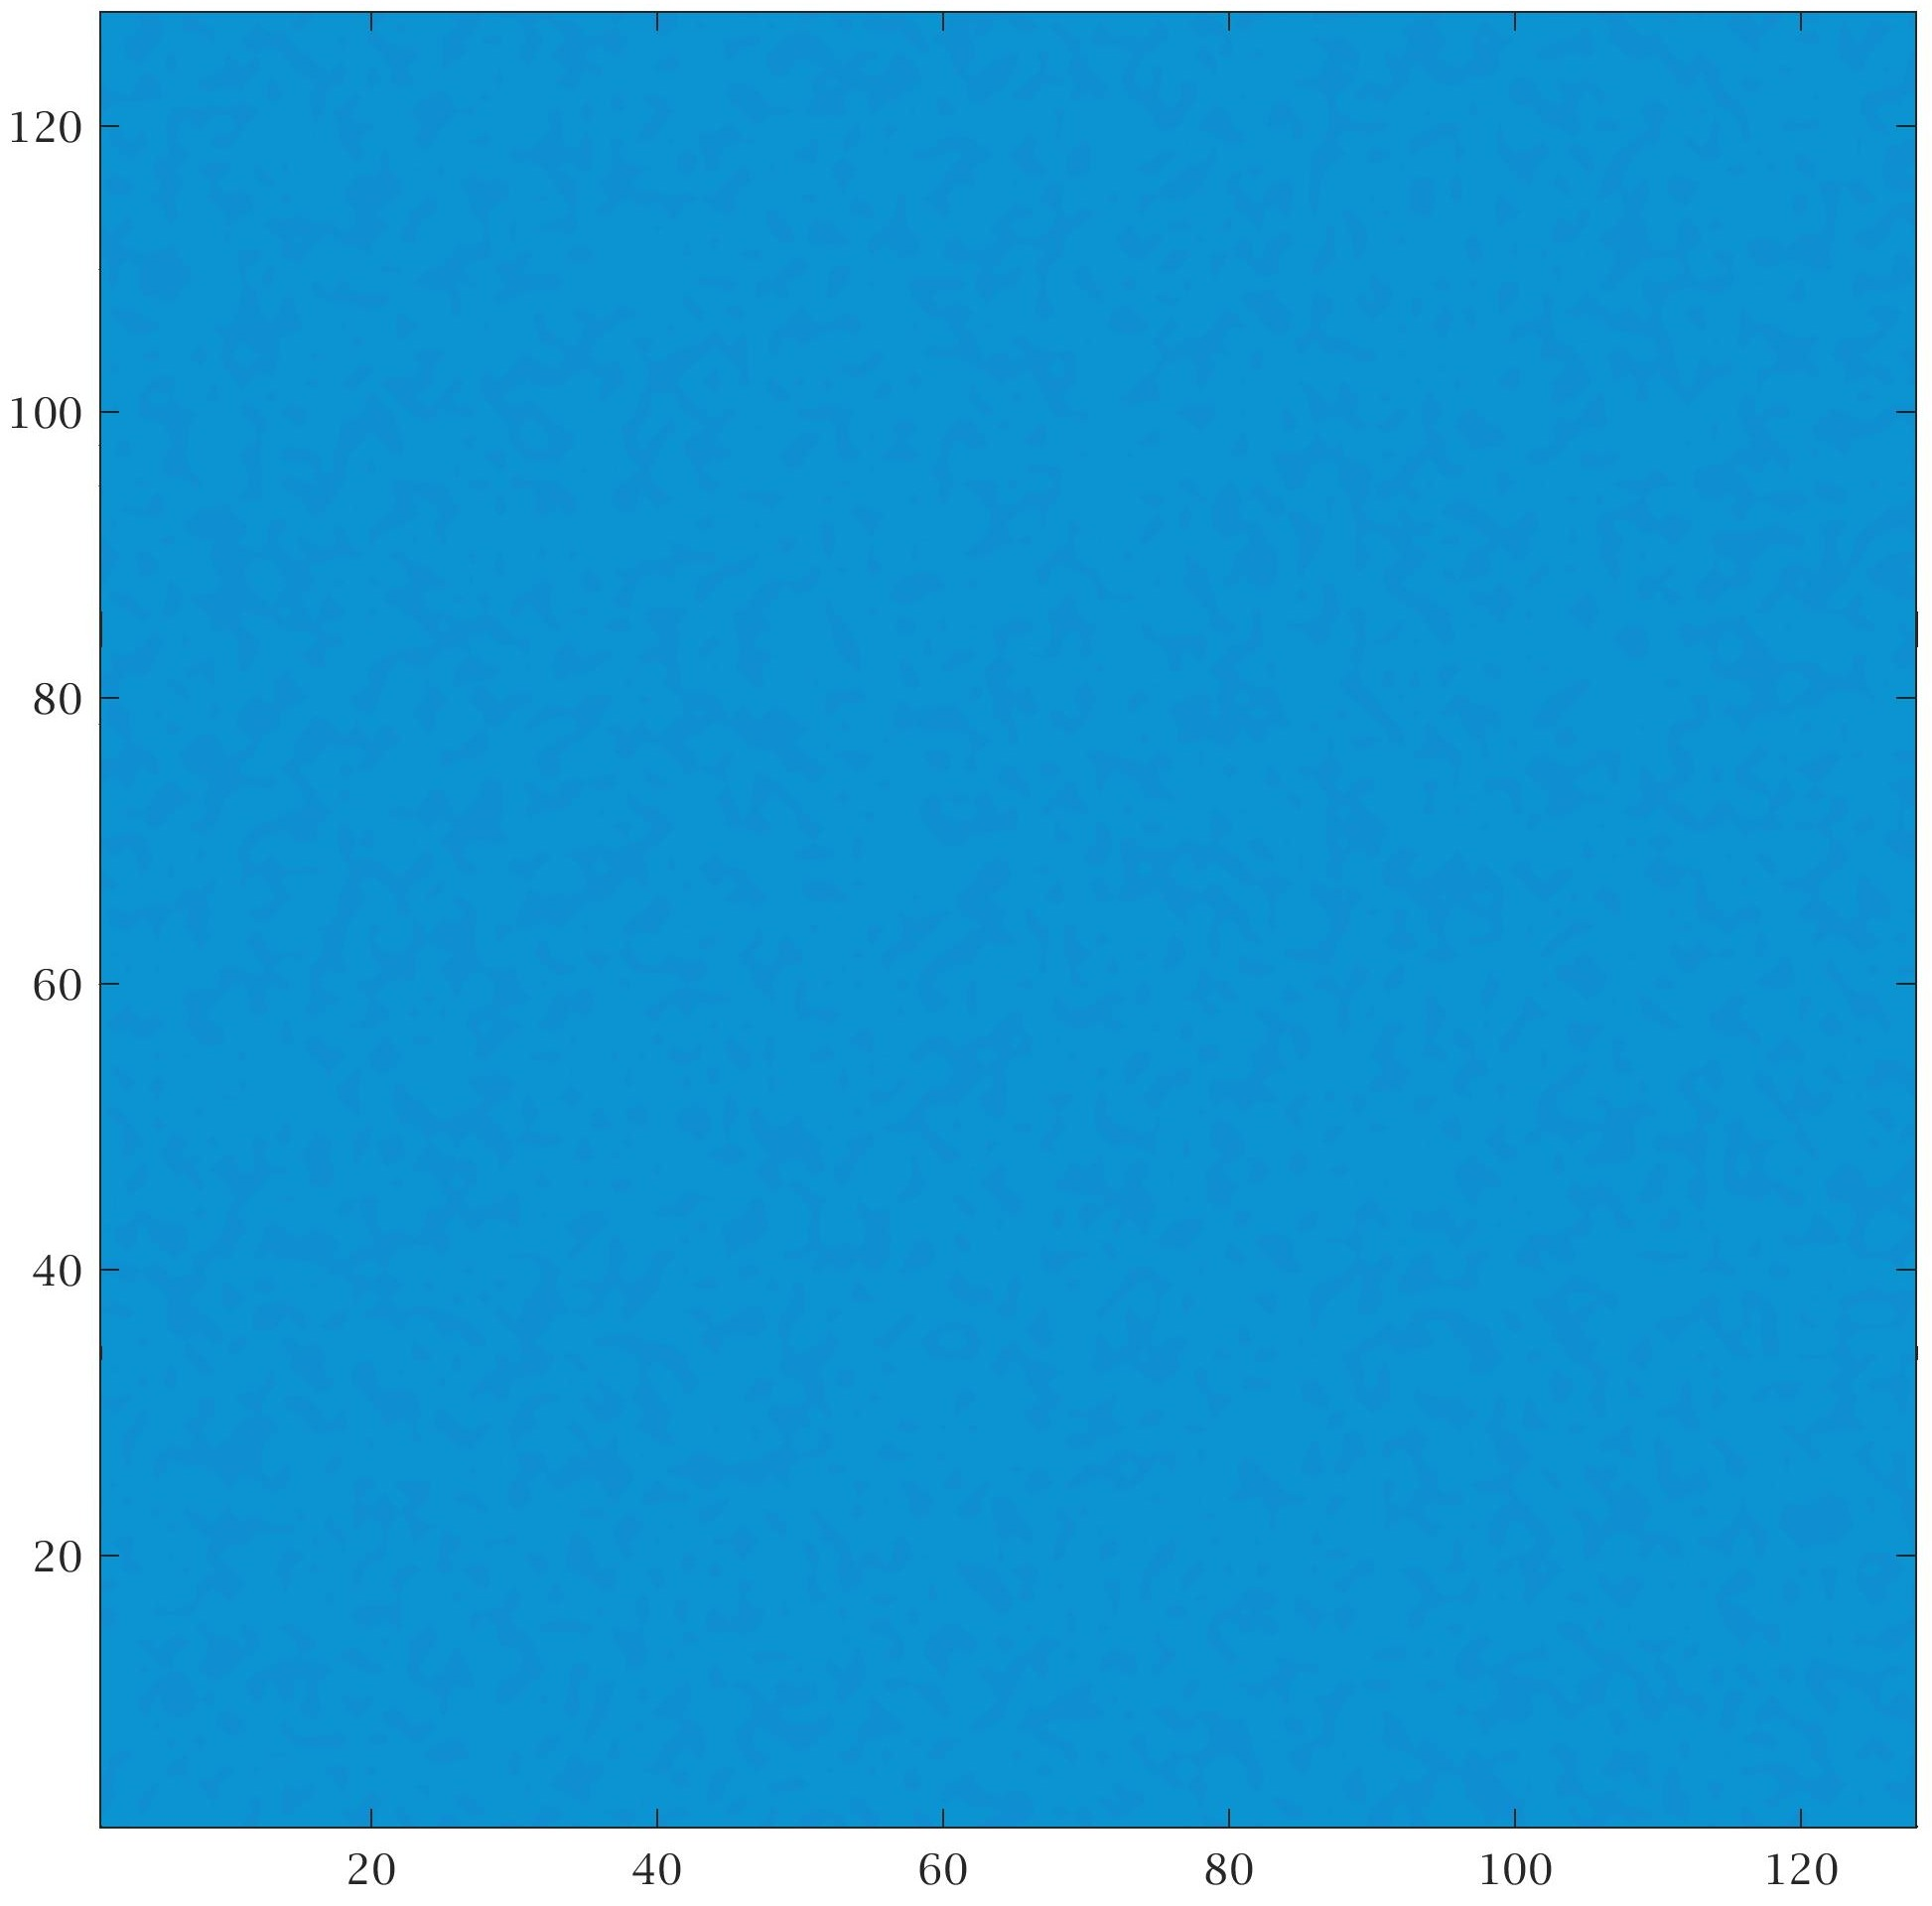
\includegraphics[width=1\textwidth]{pics/C1_t1.jpg}
                \subcaption{$t=0$}
        \end{minipage}
        %   \hfill
        \begin{minipage}[b]{.32\linewidth}
                \centering
                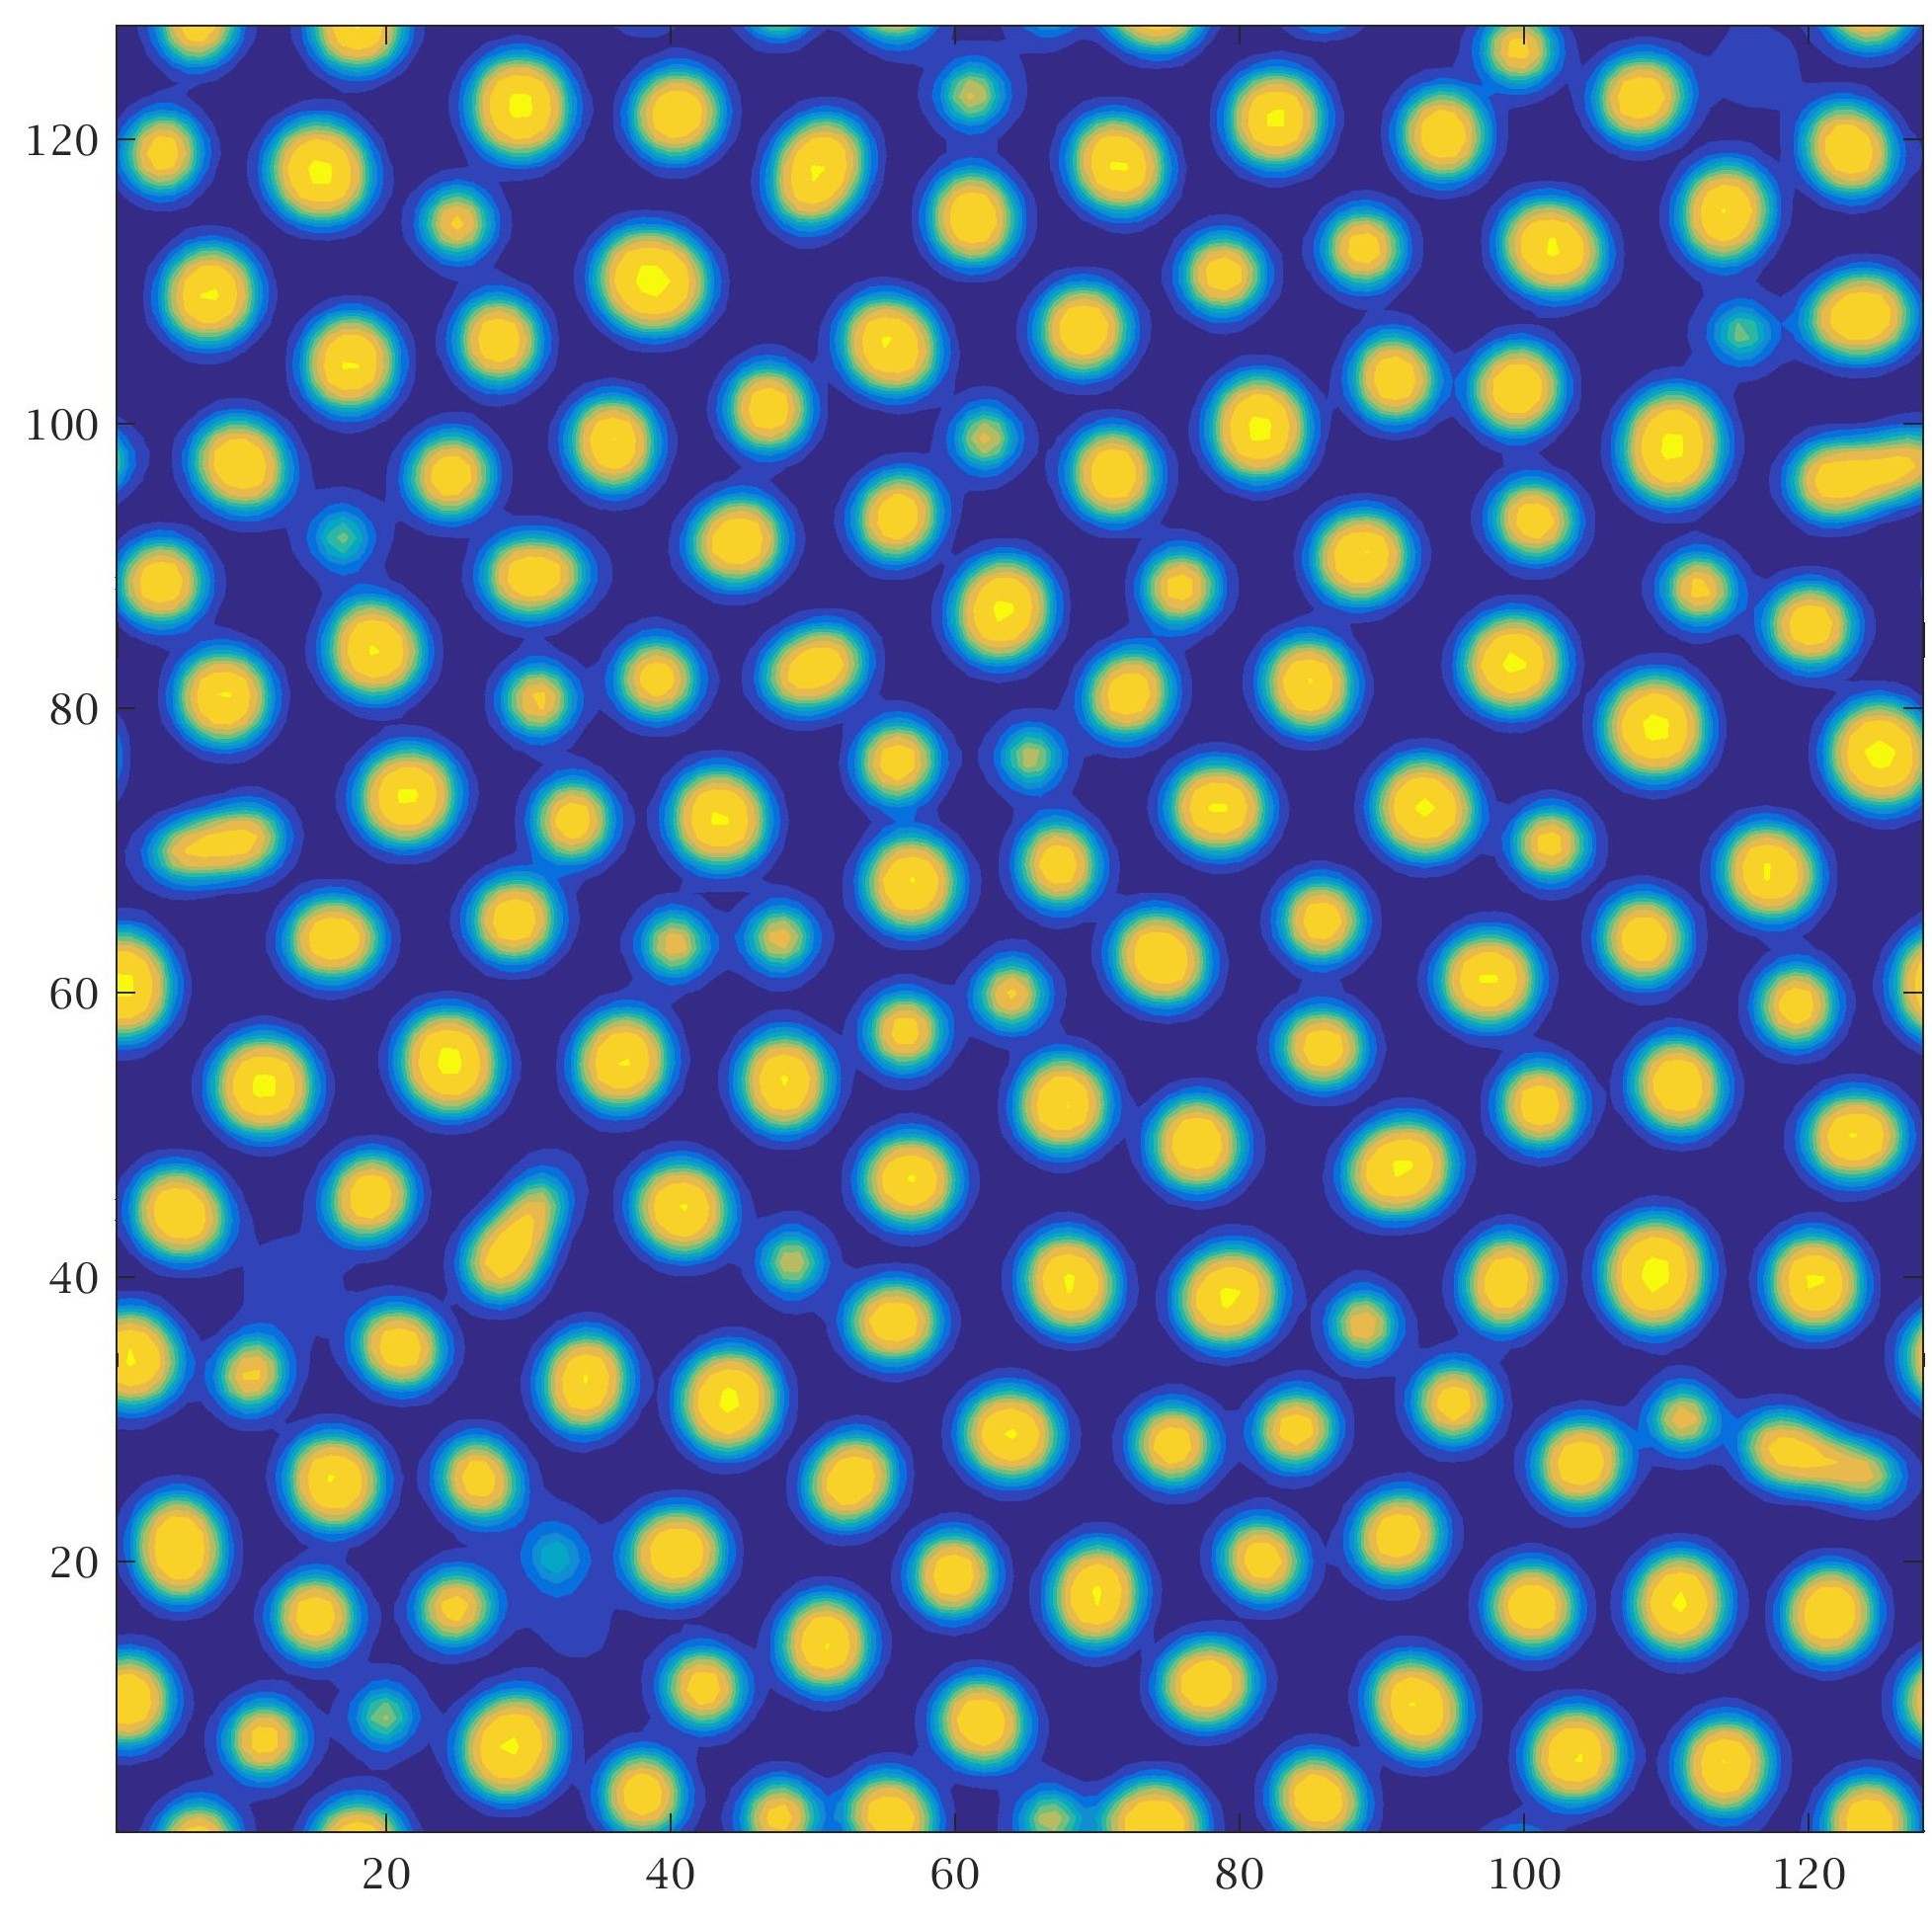
\includegraphics[width=1\textwidth]{pics/C1_t2.jpg}
                \subcaption{$t=4$}
        \end{minipage}
                \begin{minipage}[b]{.32\linewidth}
                \centering
                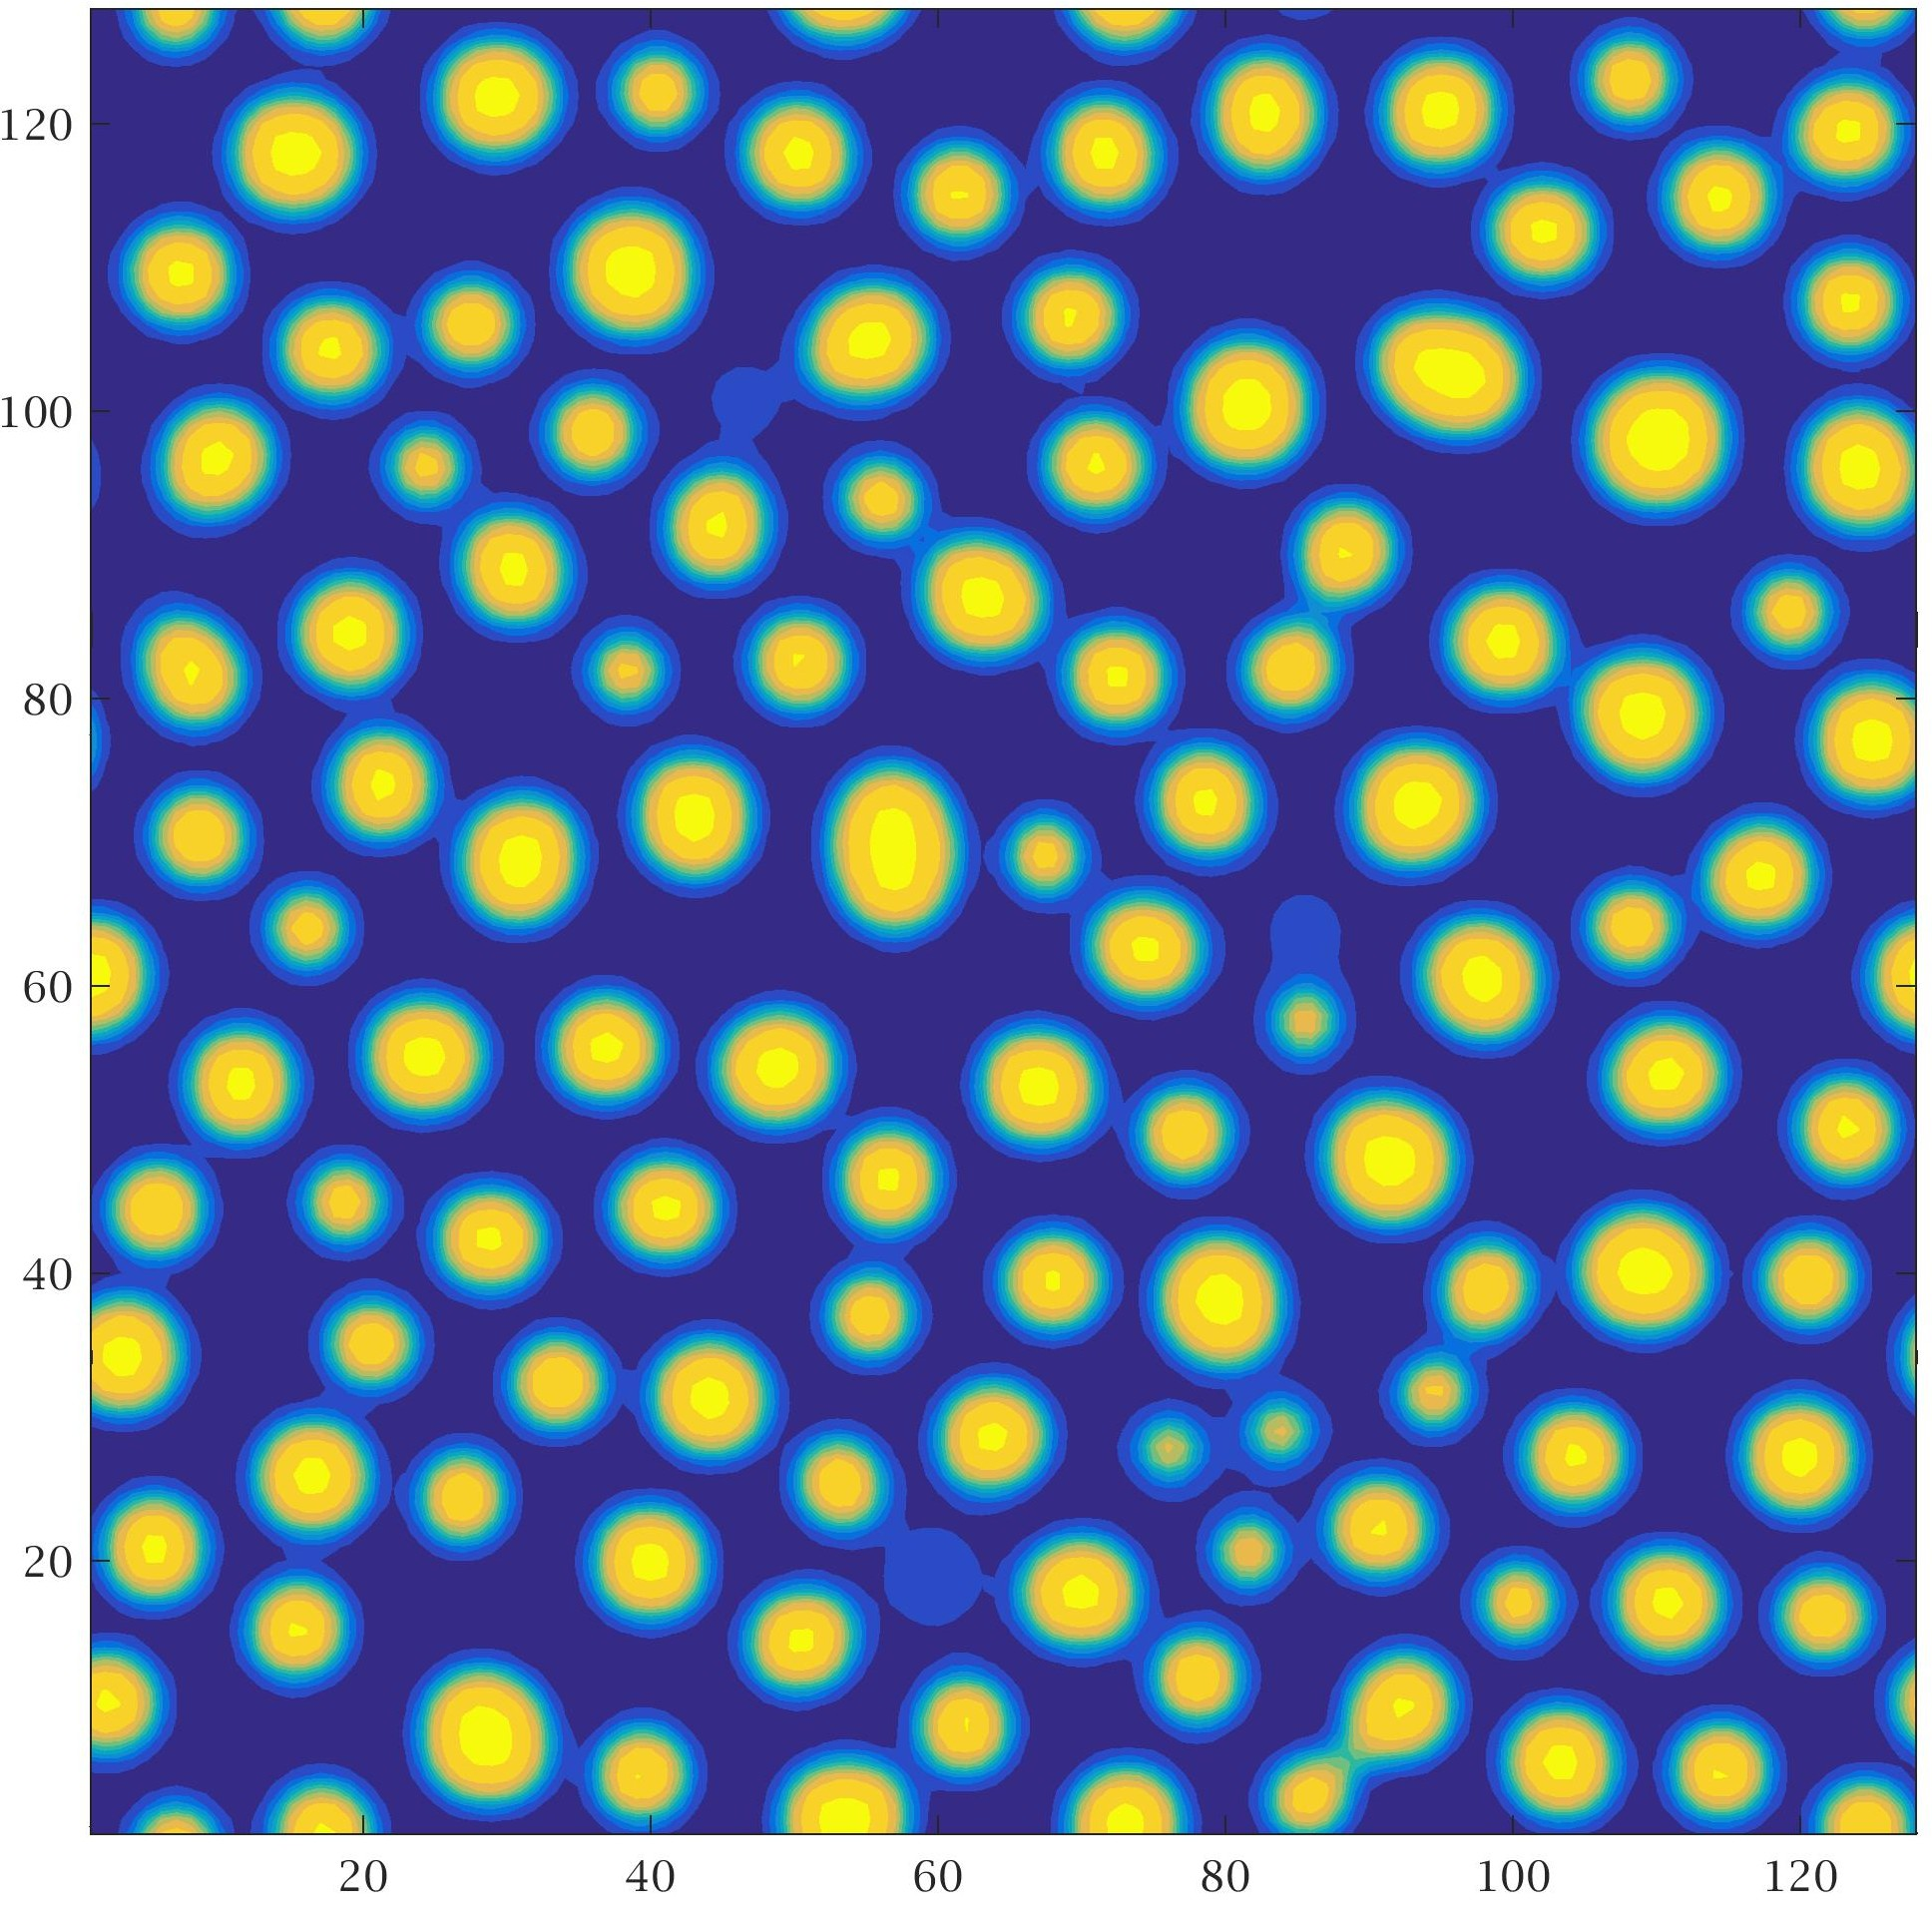
\includegraphics[width=1\textwidth]{pics/C1_t3.jpg}
                \subcaption{$t=10$}
        \end{minipage}
        
        \begin{minipage}[b]{.32\linewidth}        
                \centering
                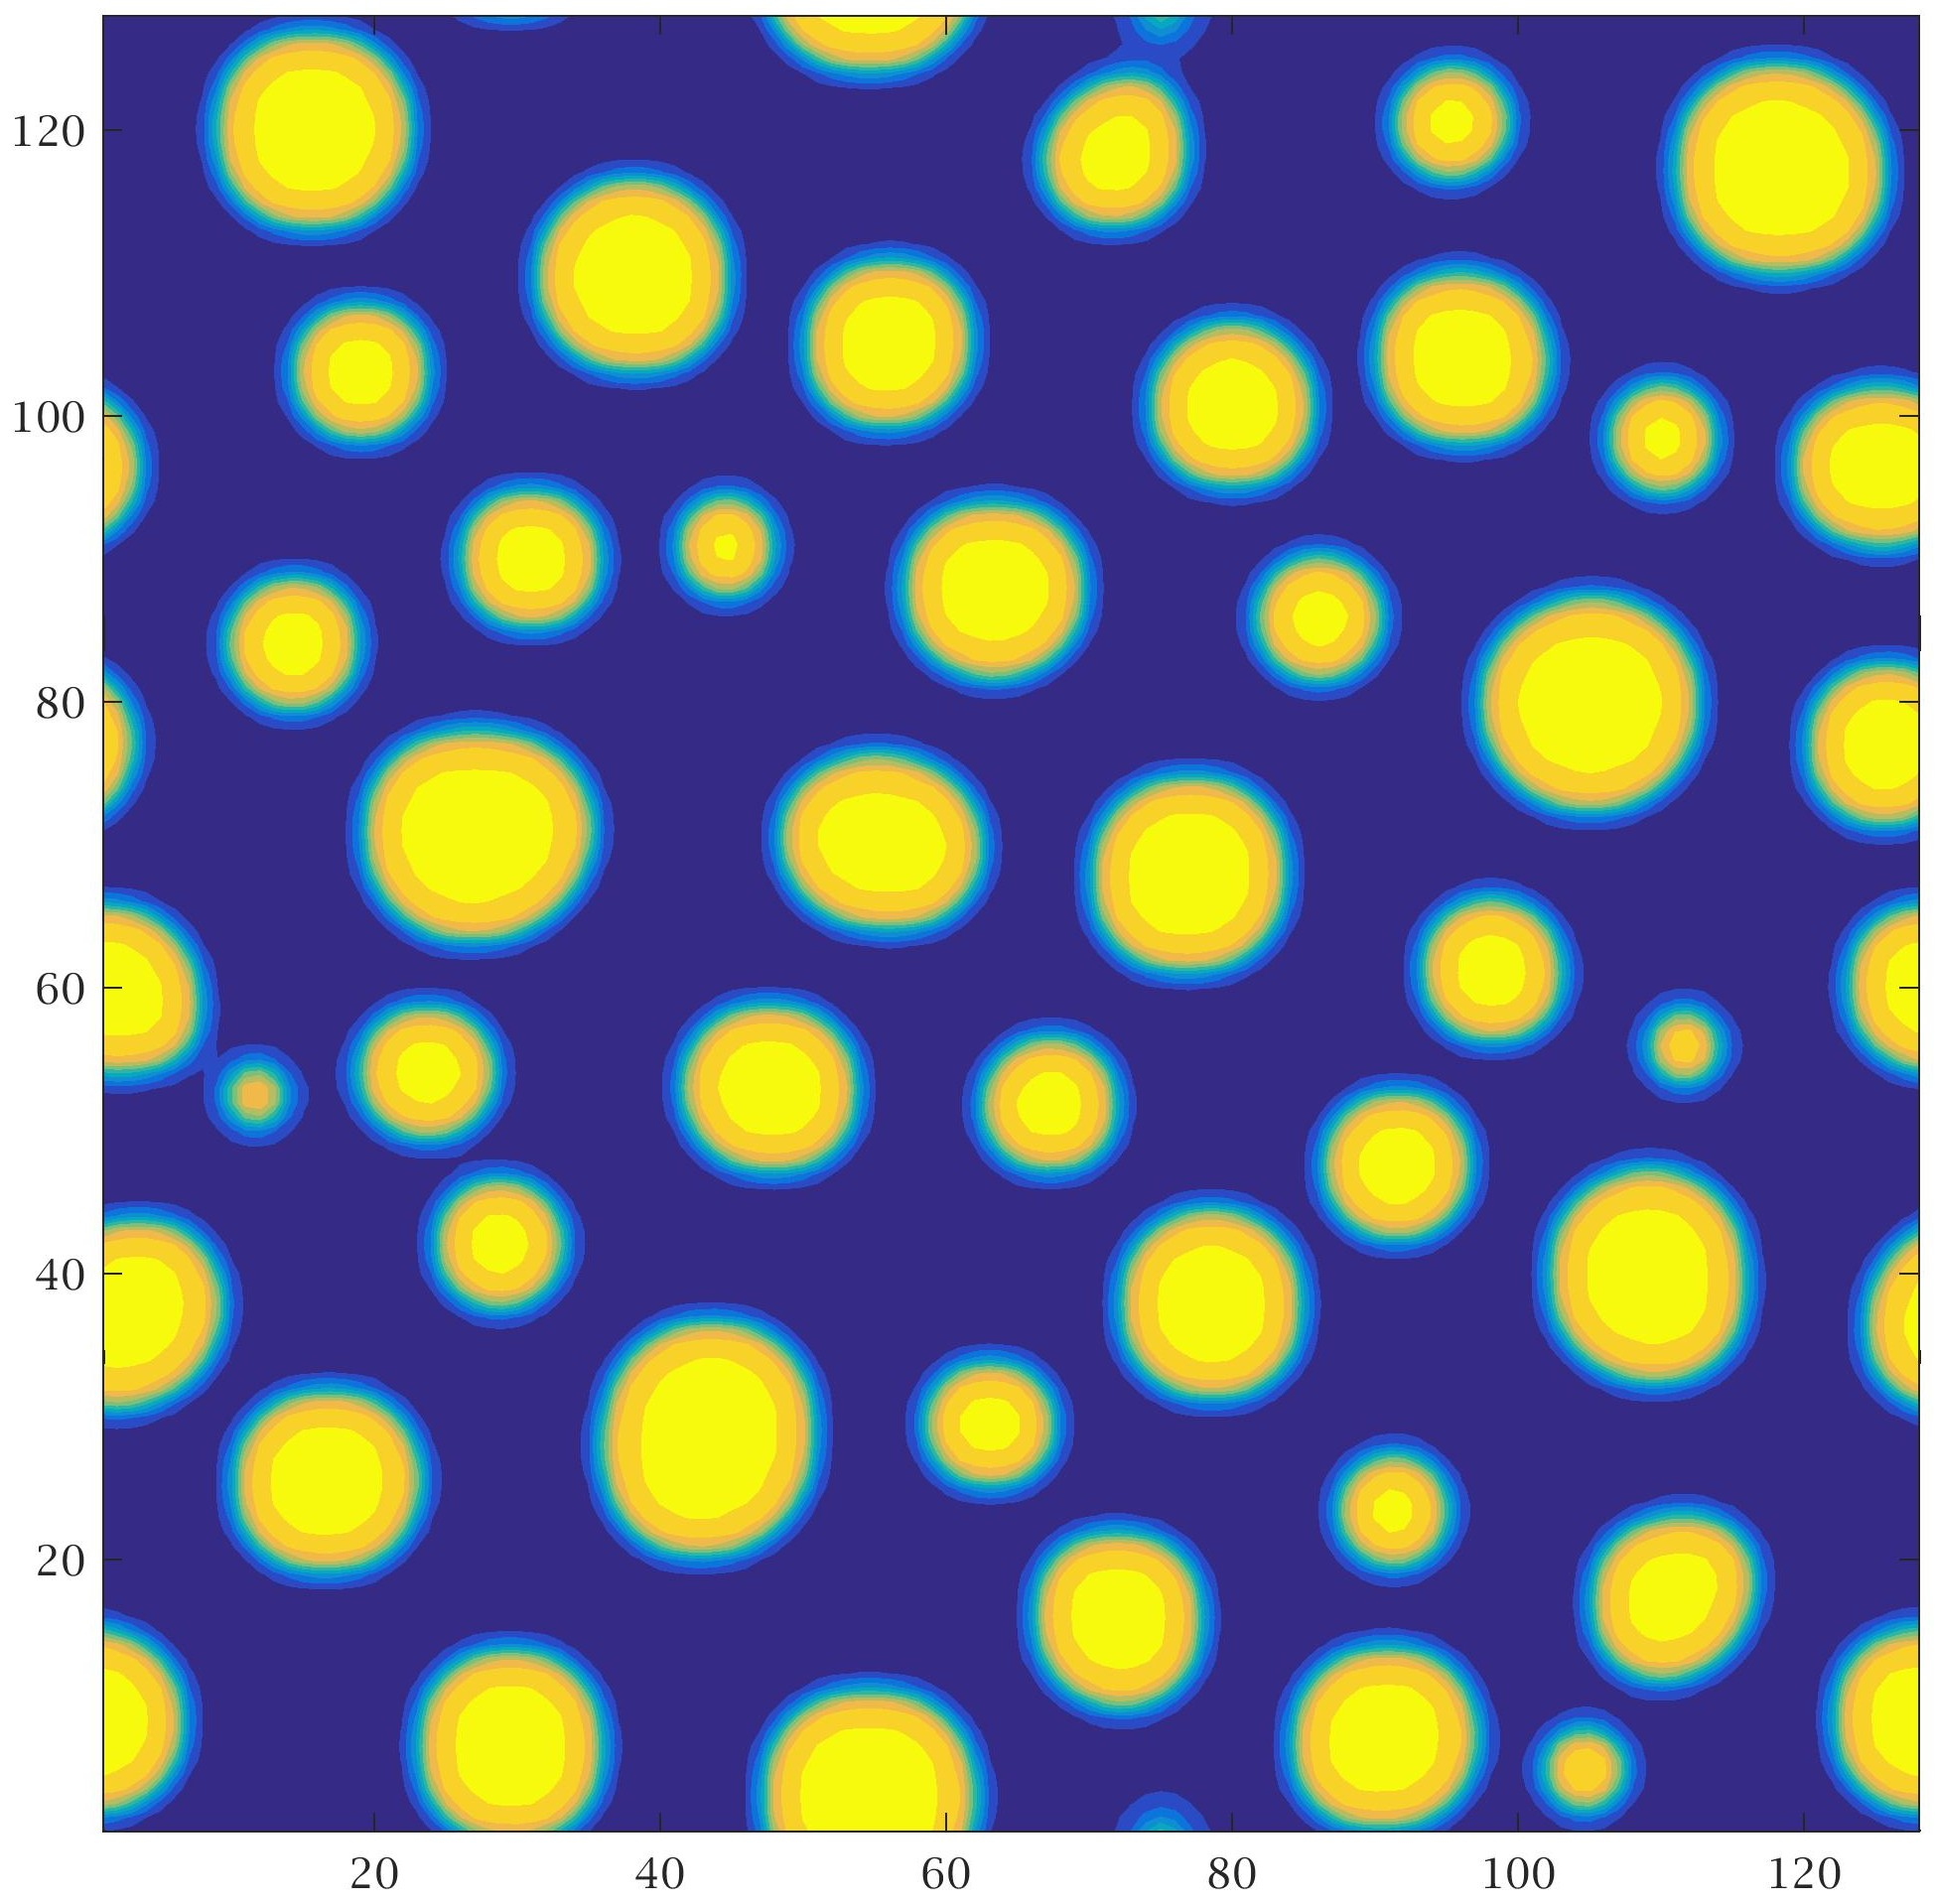
\includegraphics[width=1\textwidth]{pics/C1_t4.jpg}
                \subcaption{$t=50$}
        \end{minipage}
        %   \hfill
        \begin{minipage}[b]{.32\linewidth}
                \centering
                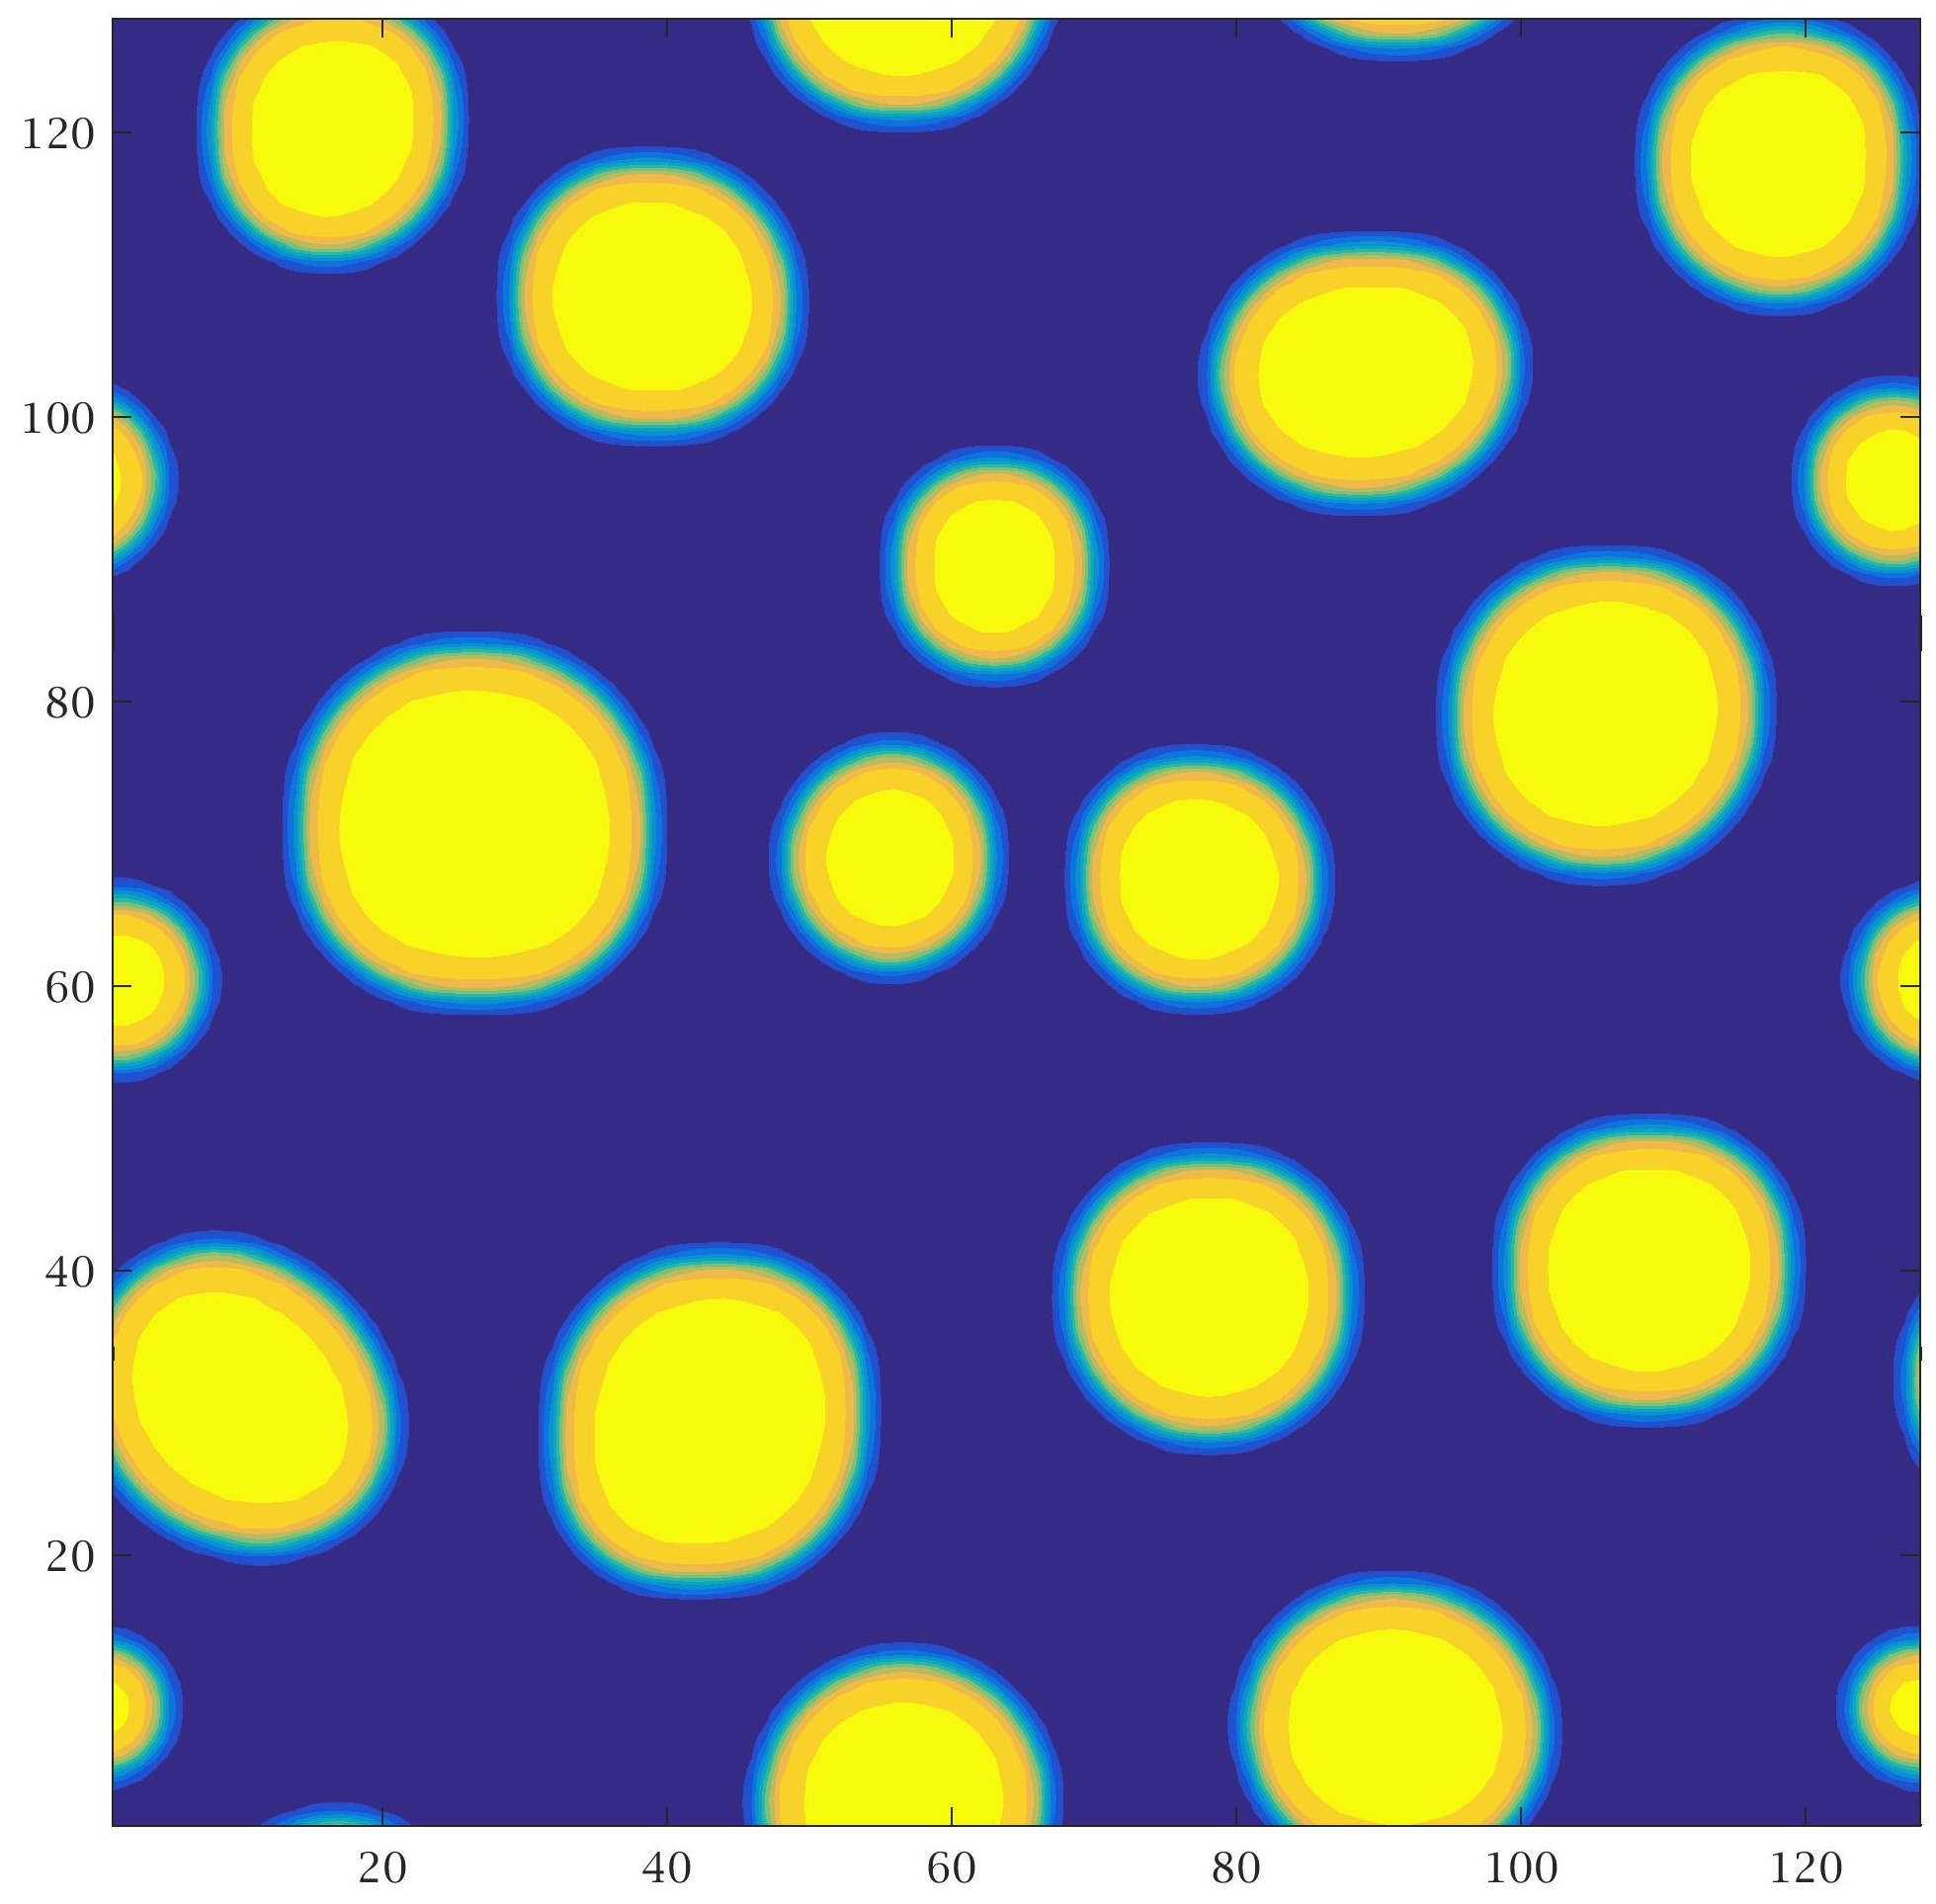
\includegraphics[width=1\textwidth]{pics/C1_t5.jpg}
                \subcaption{$t=200$}
        \end{minipage}
                \begin{minipage}[b]{.32\linewidth}
                \centering
                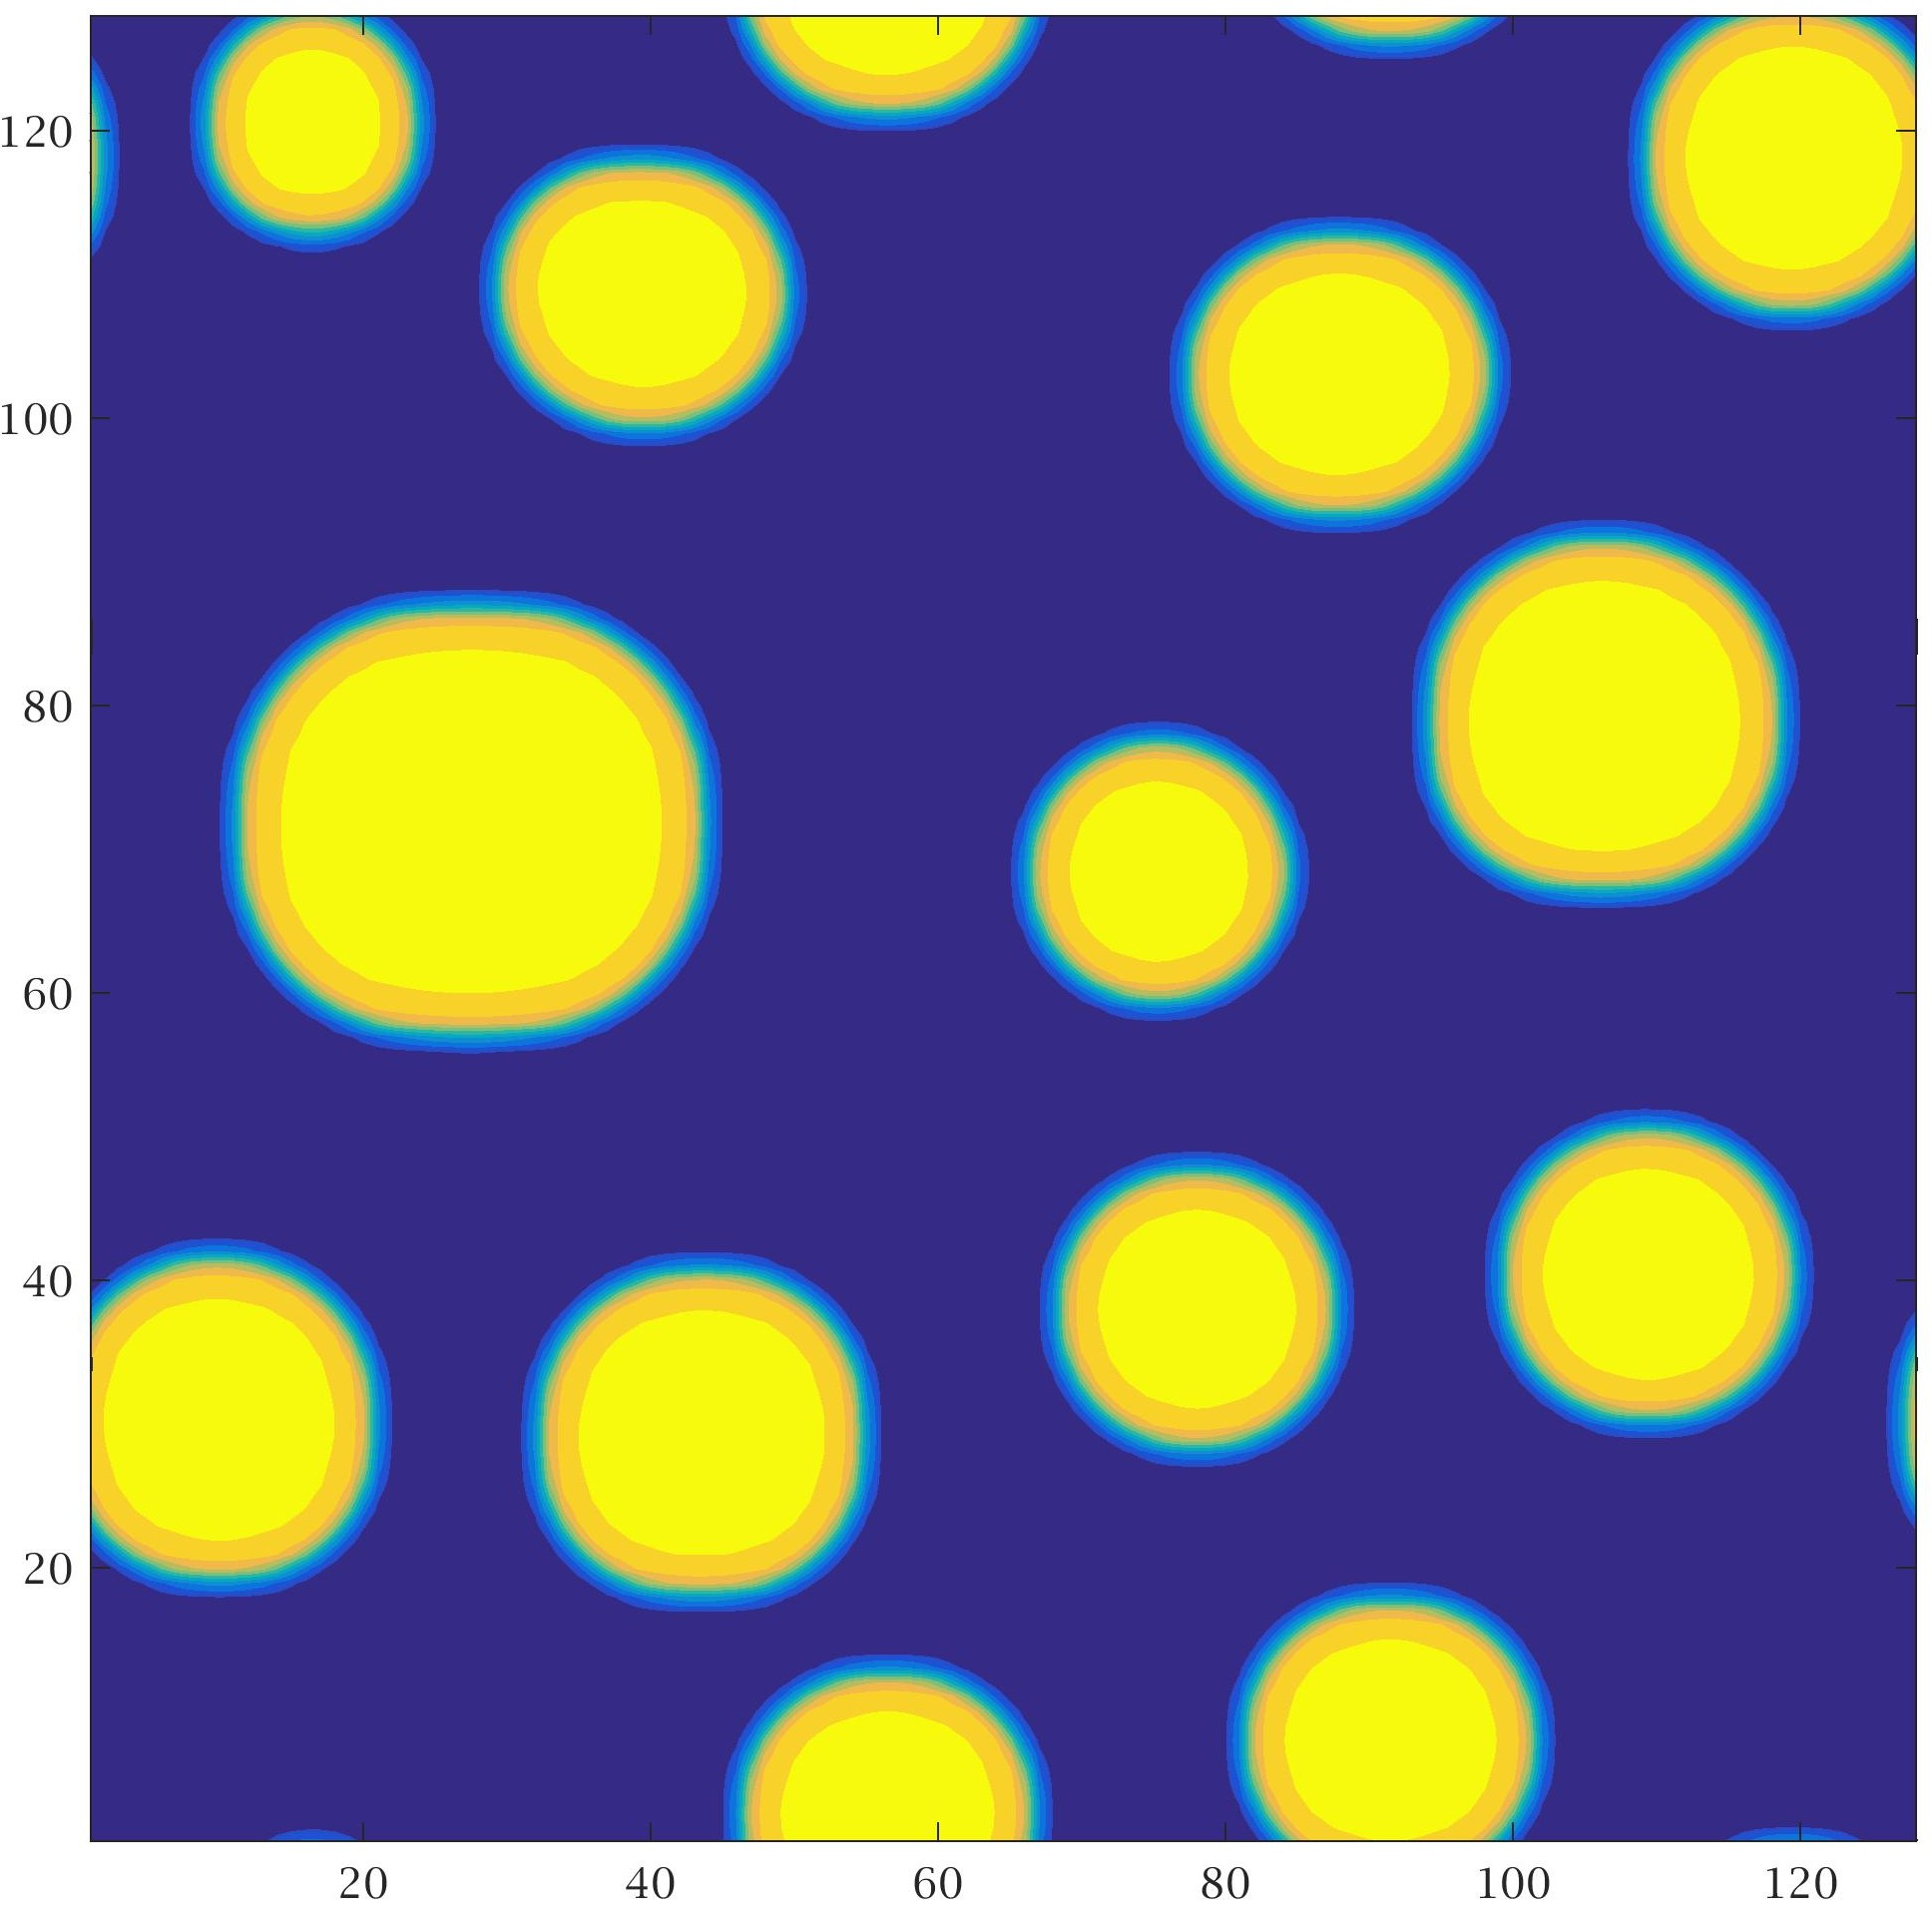
\includegraphics[width=1\textwidth]{pics/C1_t6.jpg}
                \subcaption{$t=500$}
        \end{minipage}
        \caption{Evolution with the average concentration of 0.3}
        \label{evolution_c1}
\end{figure}

Figures (\ref{E_c1} \& \ref{L_c1}) also shows the energy and characteristic length as the function of time for three different runs with the average concentration on 0.3.

Figure (\ref{E_c1}) demonstrates that the energy decreases at a rate between $t^{-1/4}$ and $t^{-1/3}$; however, figure (\ref{L_c1}) shows that the characteristic length grows at a rate between $t^{1/4}$ and $t^{1/3}$.

\begin{figure}[H]
        \begin{minipage}[b]{.5\linewidth}       
                \centering
                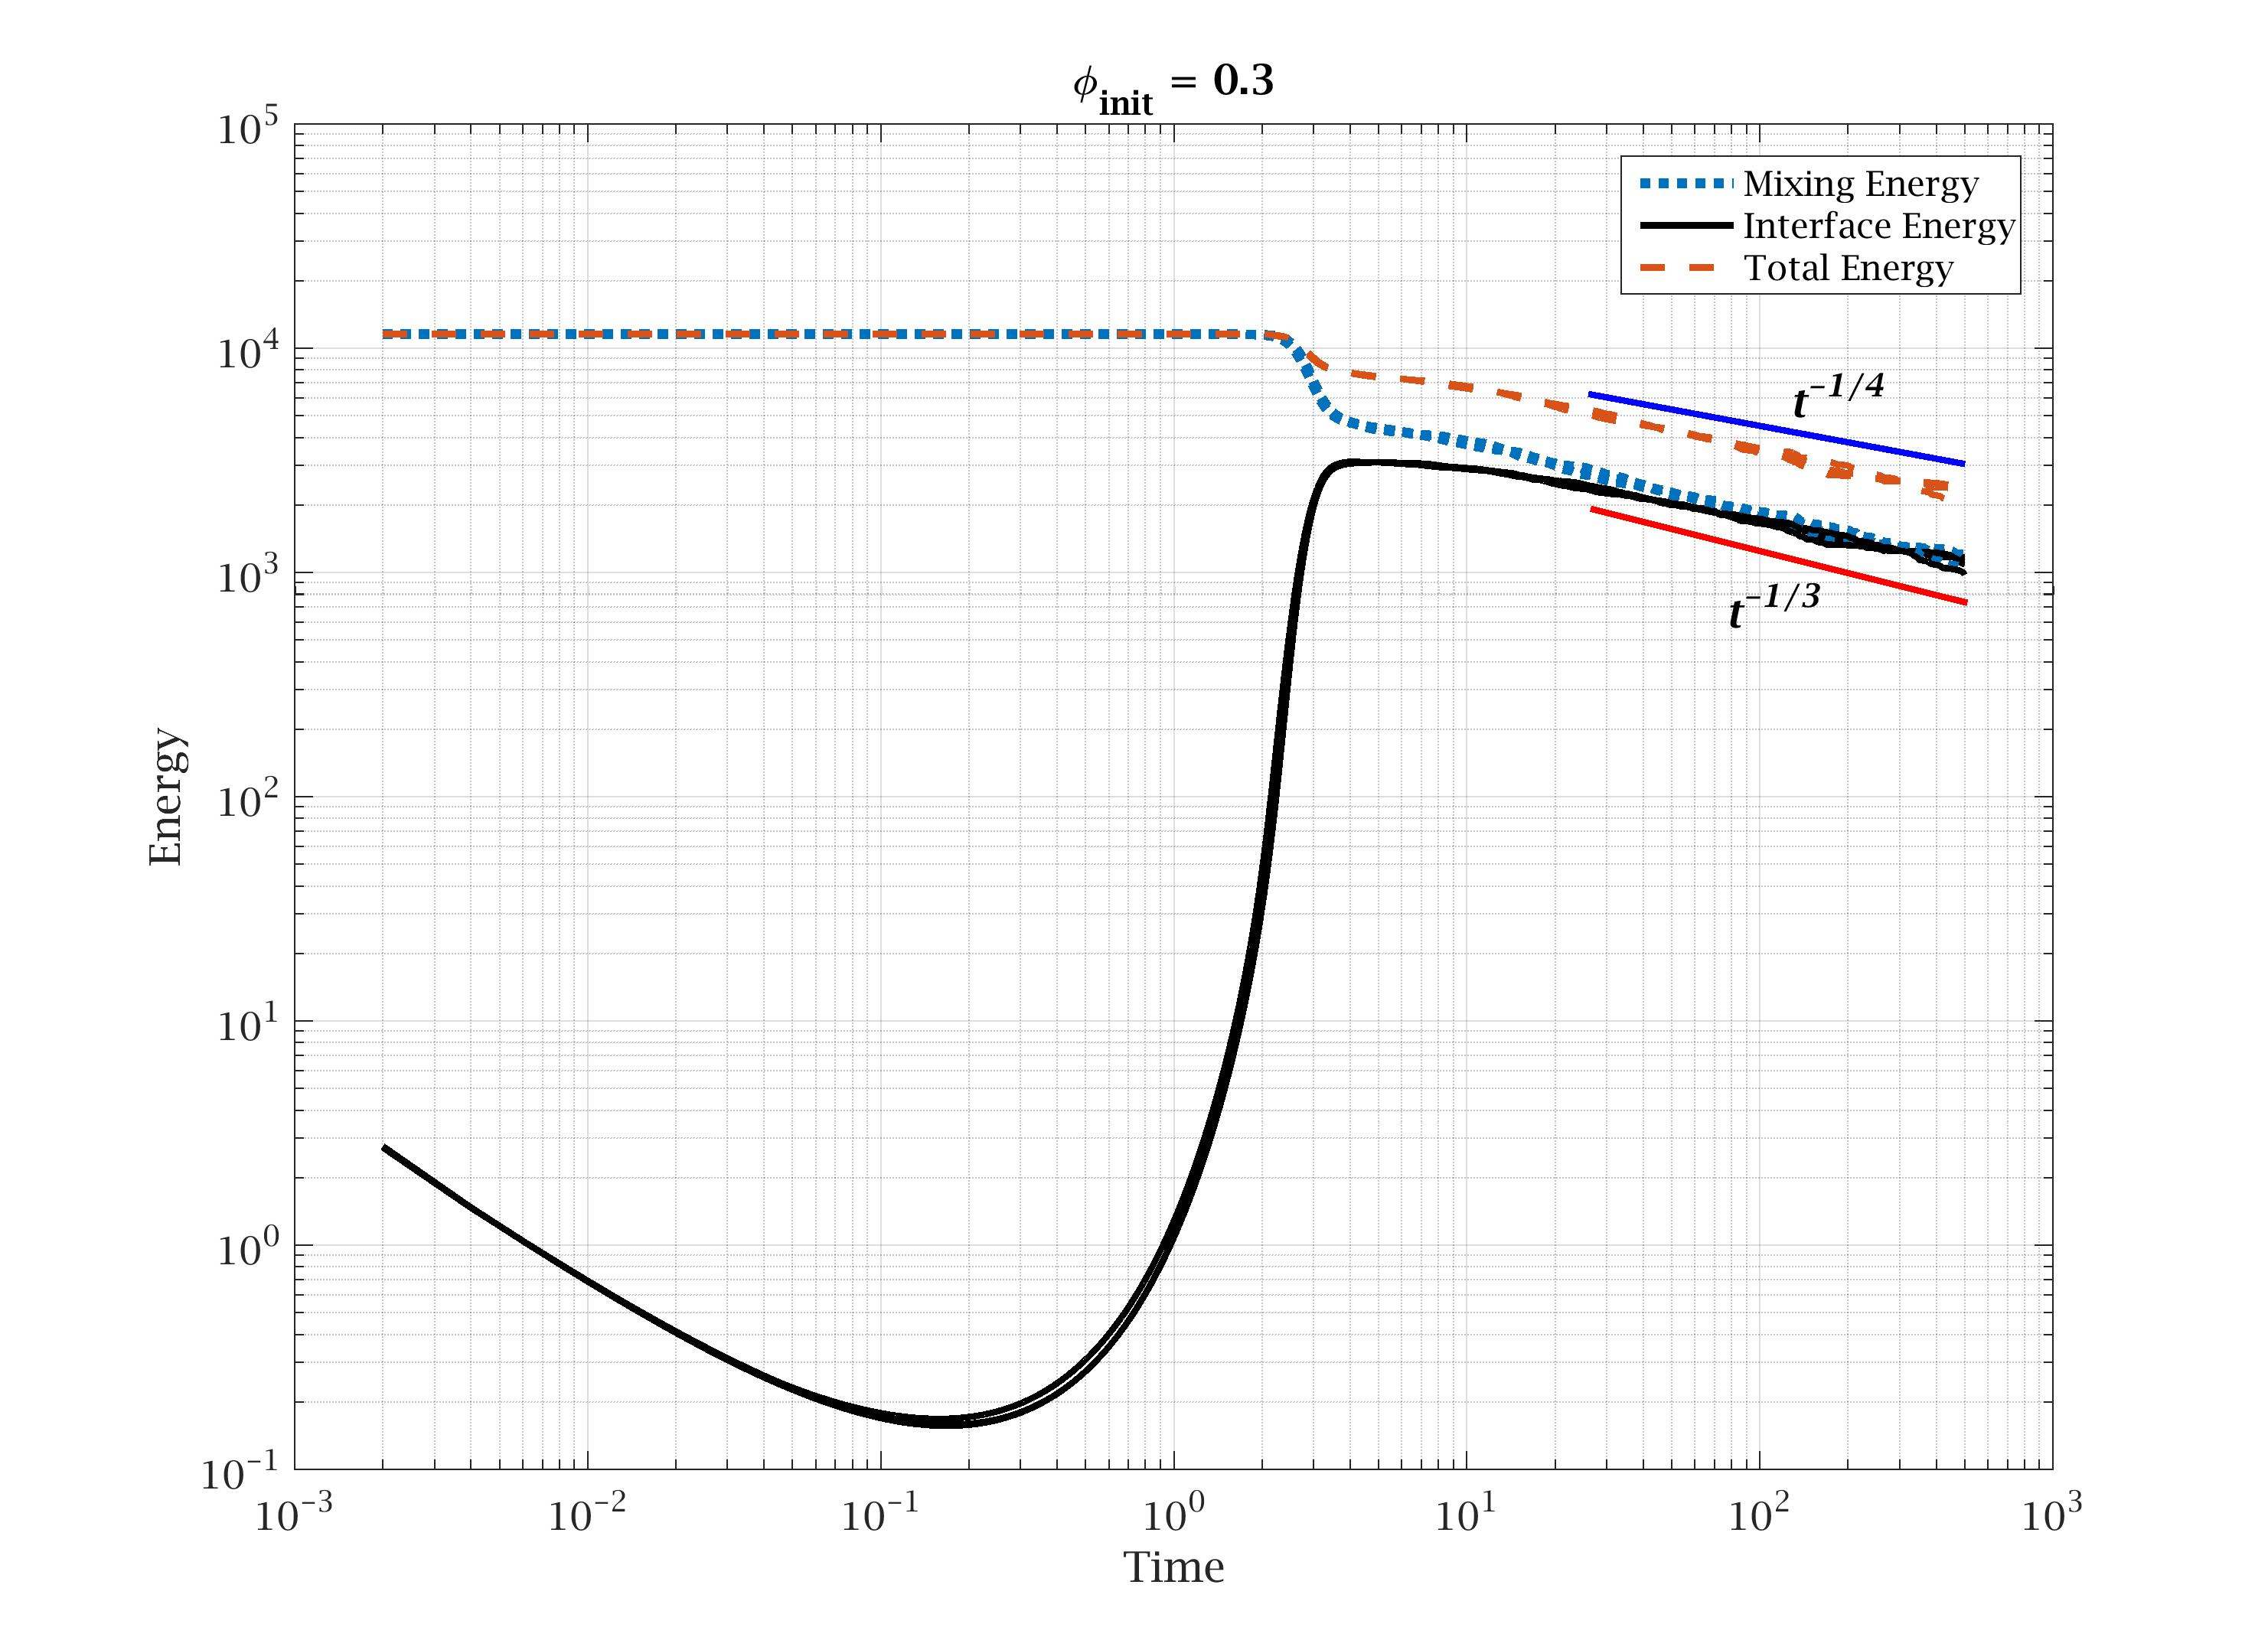
\includegraphics[width=1\textwidth]{pics/E_c1.jpg}
                \subcaption{}
                \label{E_c1} 
        \end{minipage}
        %   \hfill
        \begin{minipage}[b]{.5\linewidth}
                \centering
                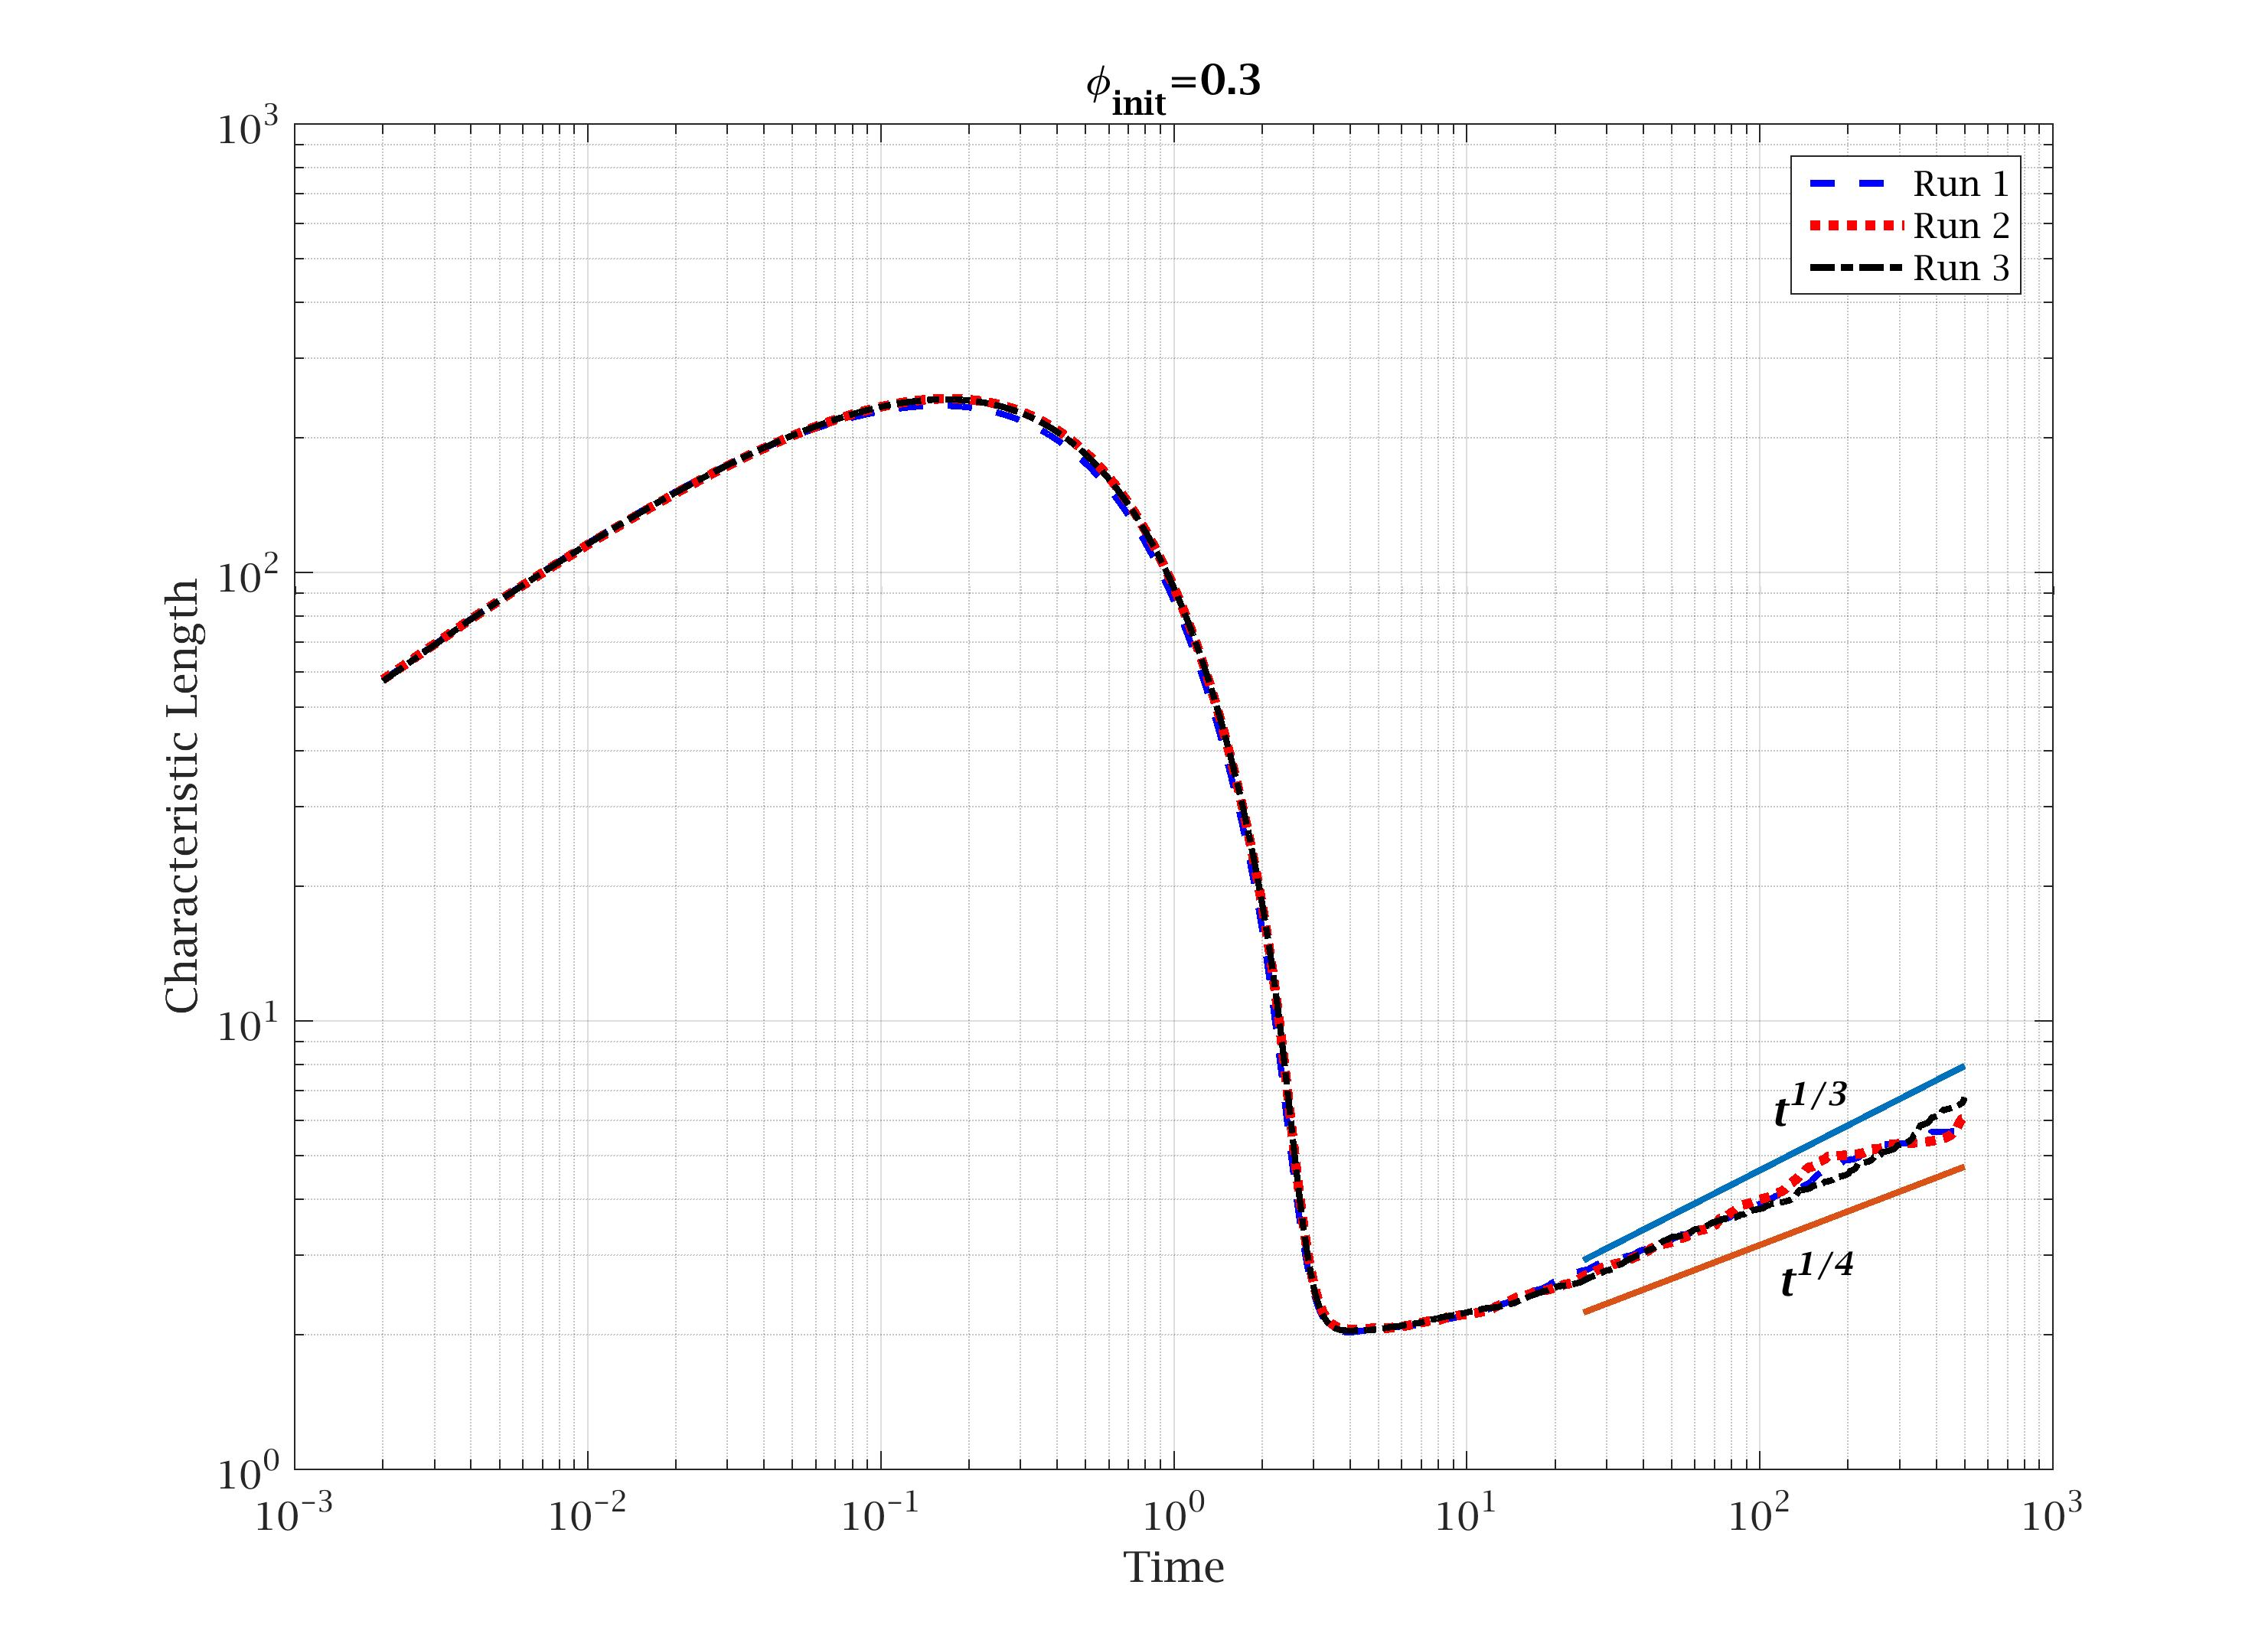
\includegraphics[width=1\textwidth]{pics/L_c1.jpg}
                \subcaption{}
                \label{L_c1}
        \end{minipage}
                \caption{The (a) interfacial, mixing and total energy and (b) characteristic length as a function of time for the average concentration of 0.3}
        \label{EL_c1}
\end{figure}

\subsection{Case 2, Ave. concentration of 0.5}

The figure (\ref{evolution_c2}) shows the evolution of the phase filed variable for the average concentration of 0.5.

\begin{figure}[H]
        \begin{minipage}[b]{.32\linewidth}        
                \centering
                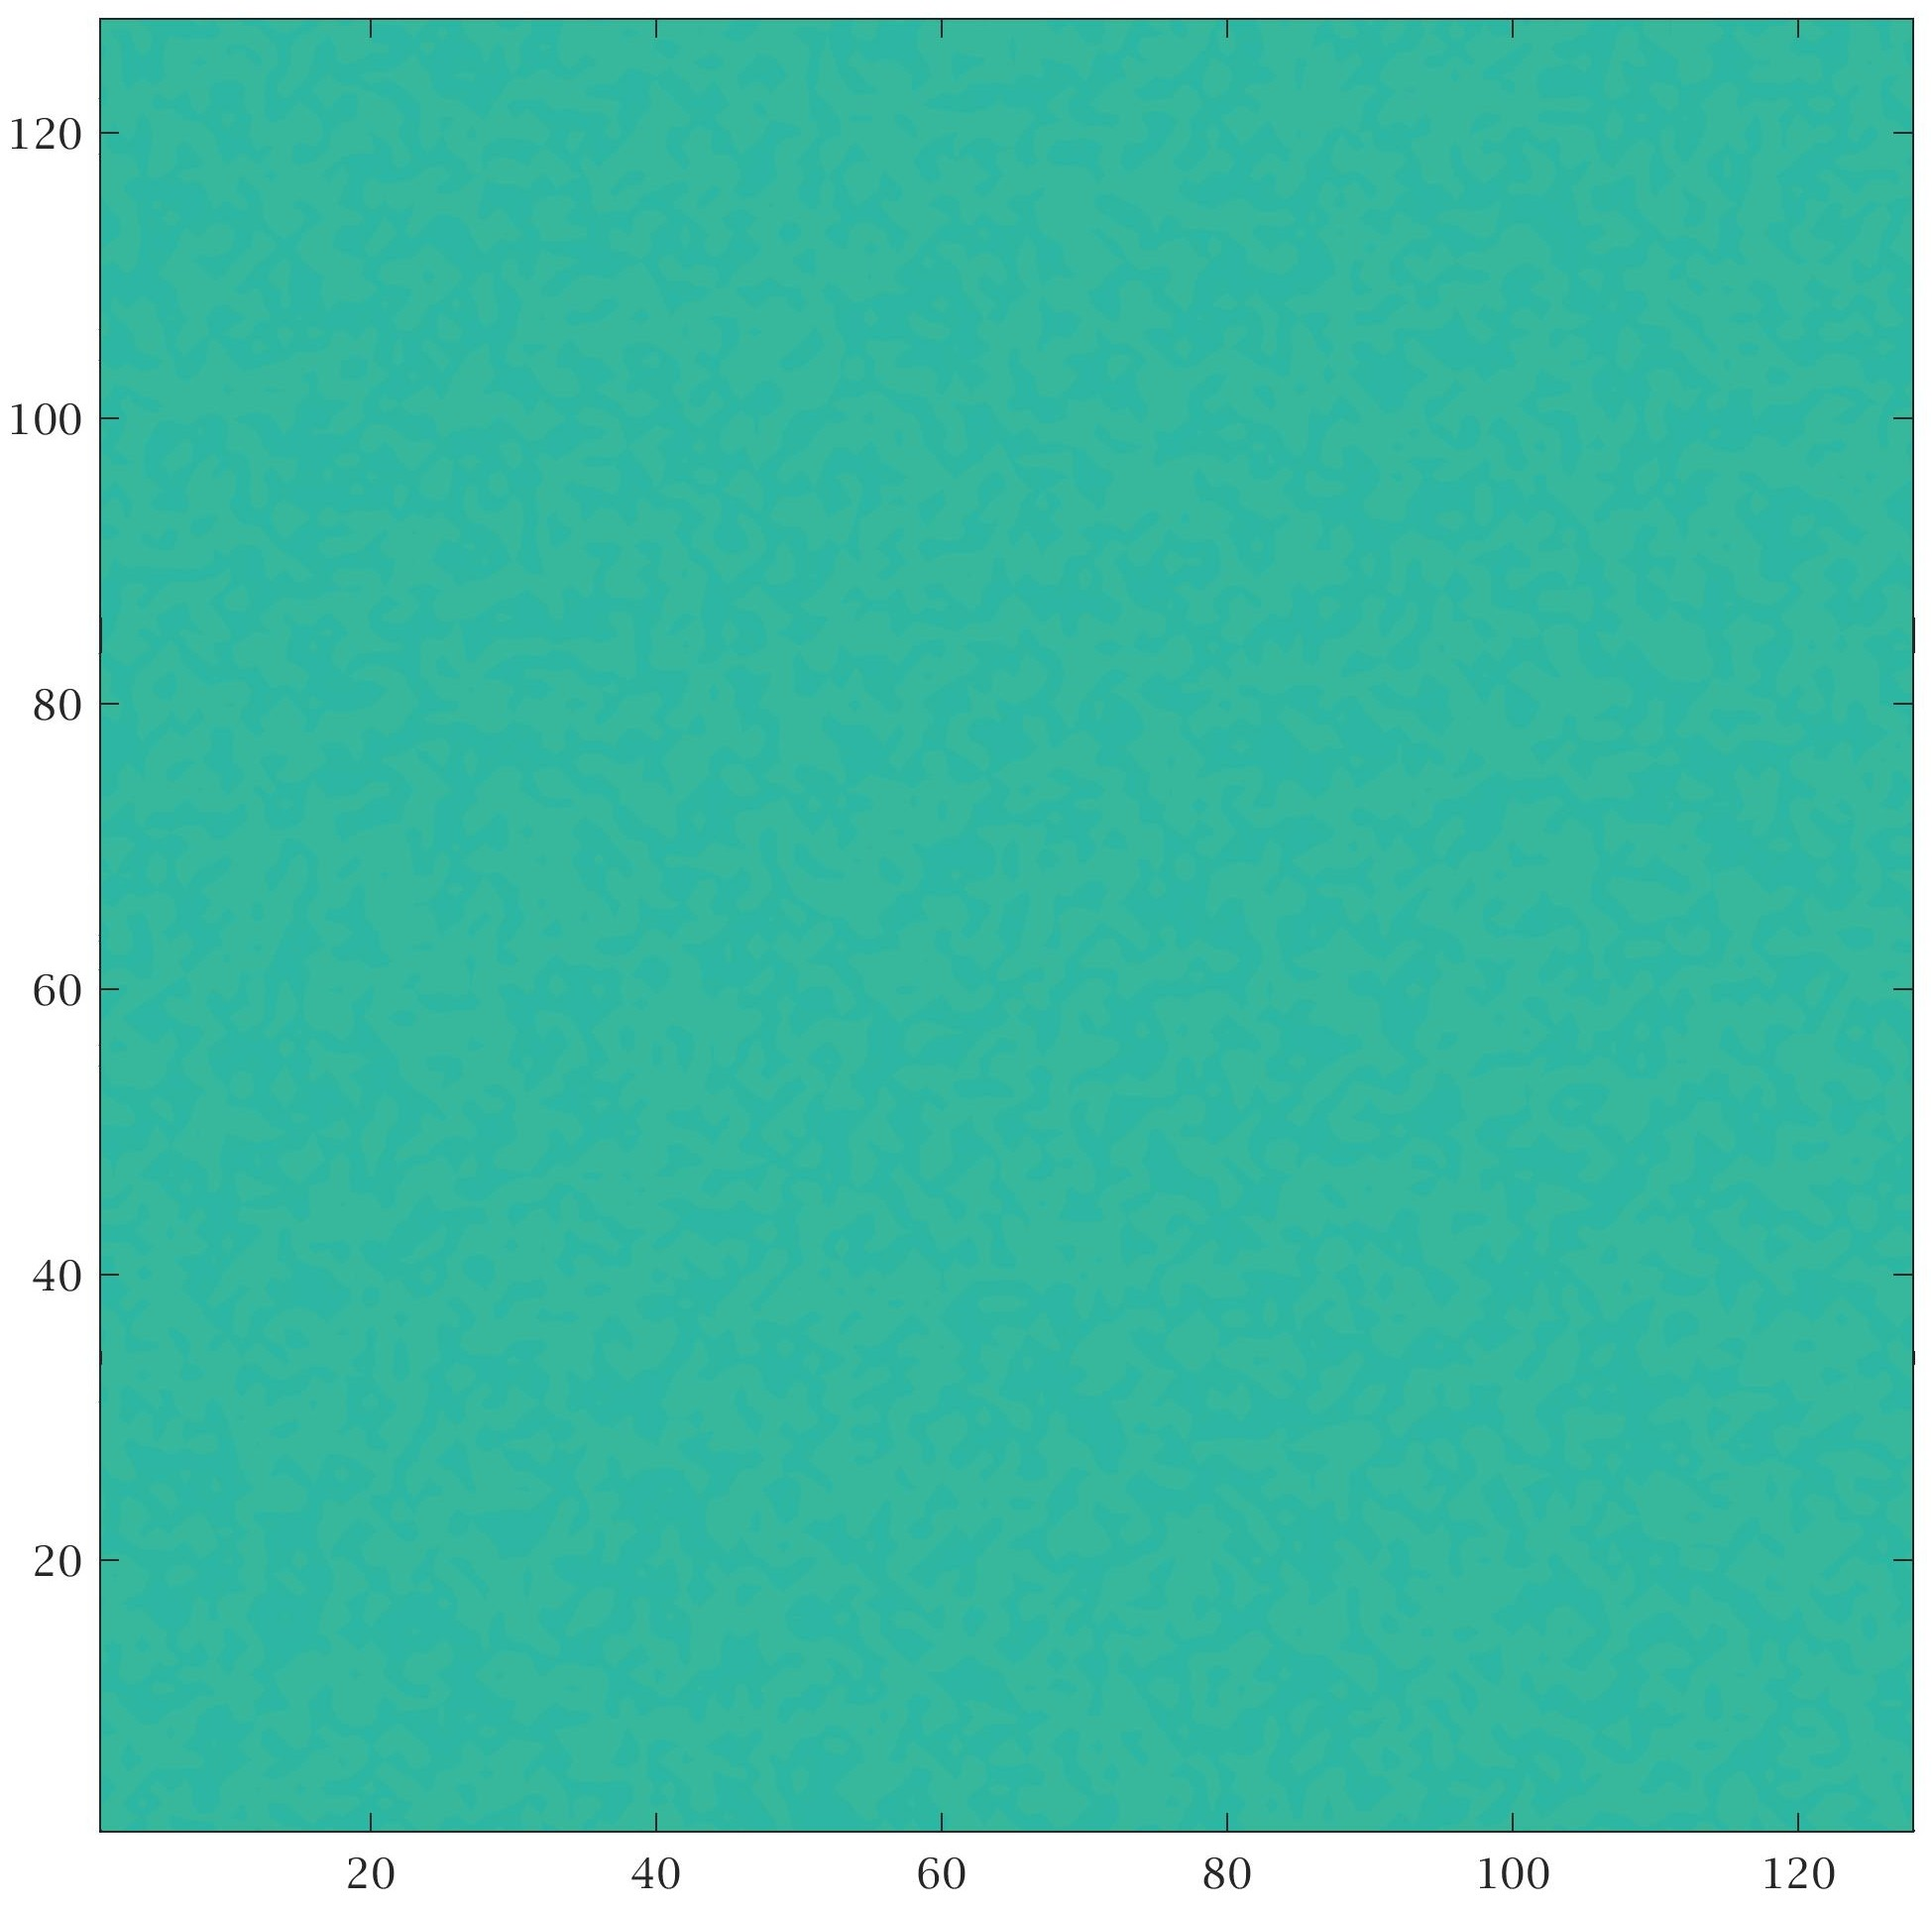
\includegraphics[width=1\textwidth]{pics/C2_t1.jpg}
                \subcaption{$t=0$}
        \end{minipage}
        %   \hfill
        \begin{minipage}[b]{.32\linewidth}
                \centering
                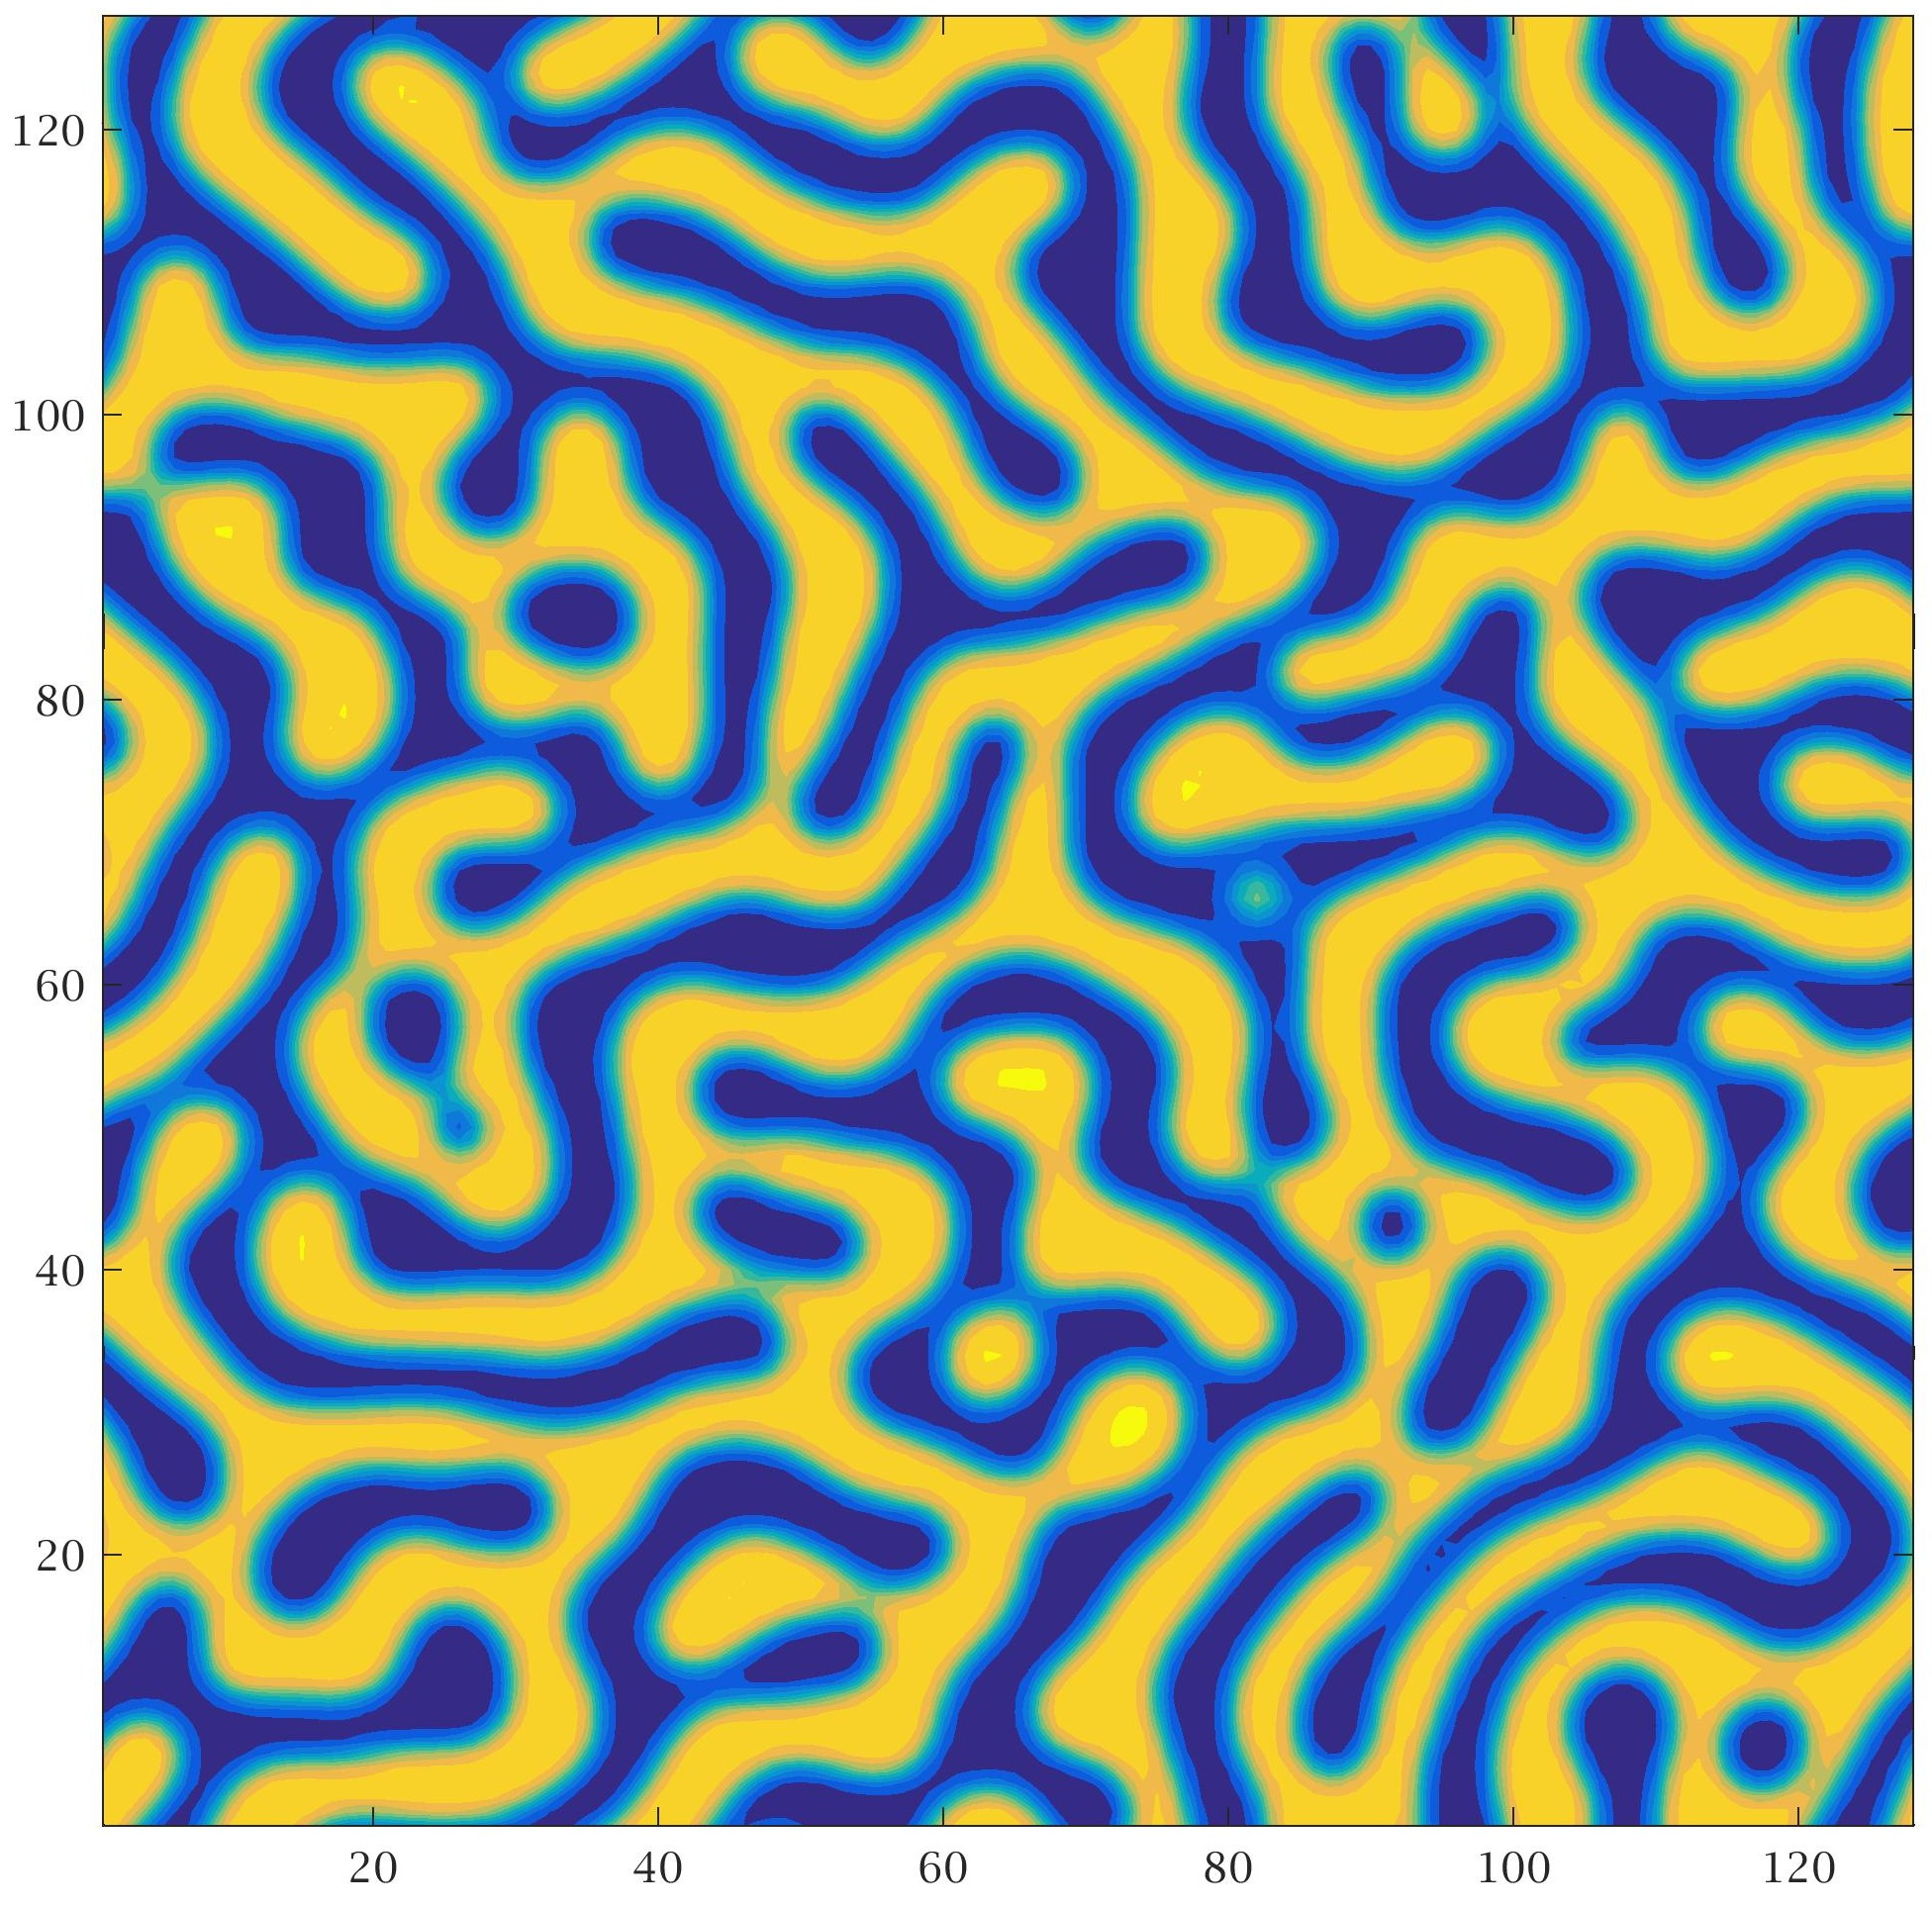
\includegraphics[width=1\textwidth]{pics/C2_t2.jpg}
                \subcaption{$t=4$}
        \end{minipage}
                \begin{minipage}[b]{.32\linewidth}
                \centering
                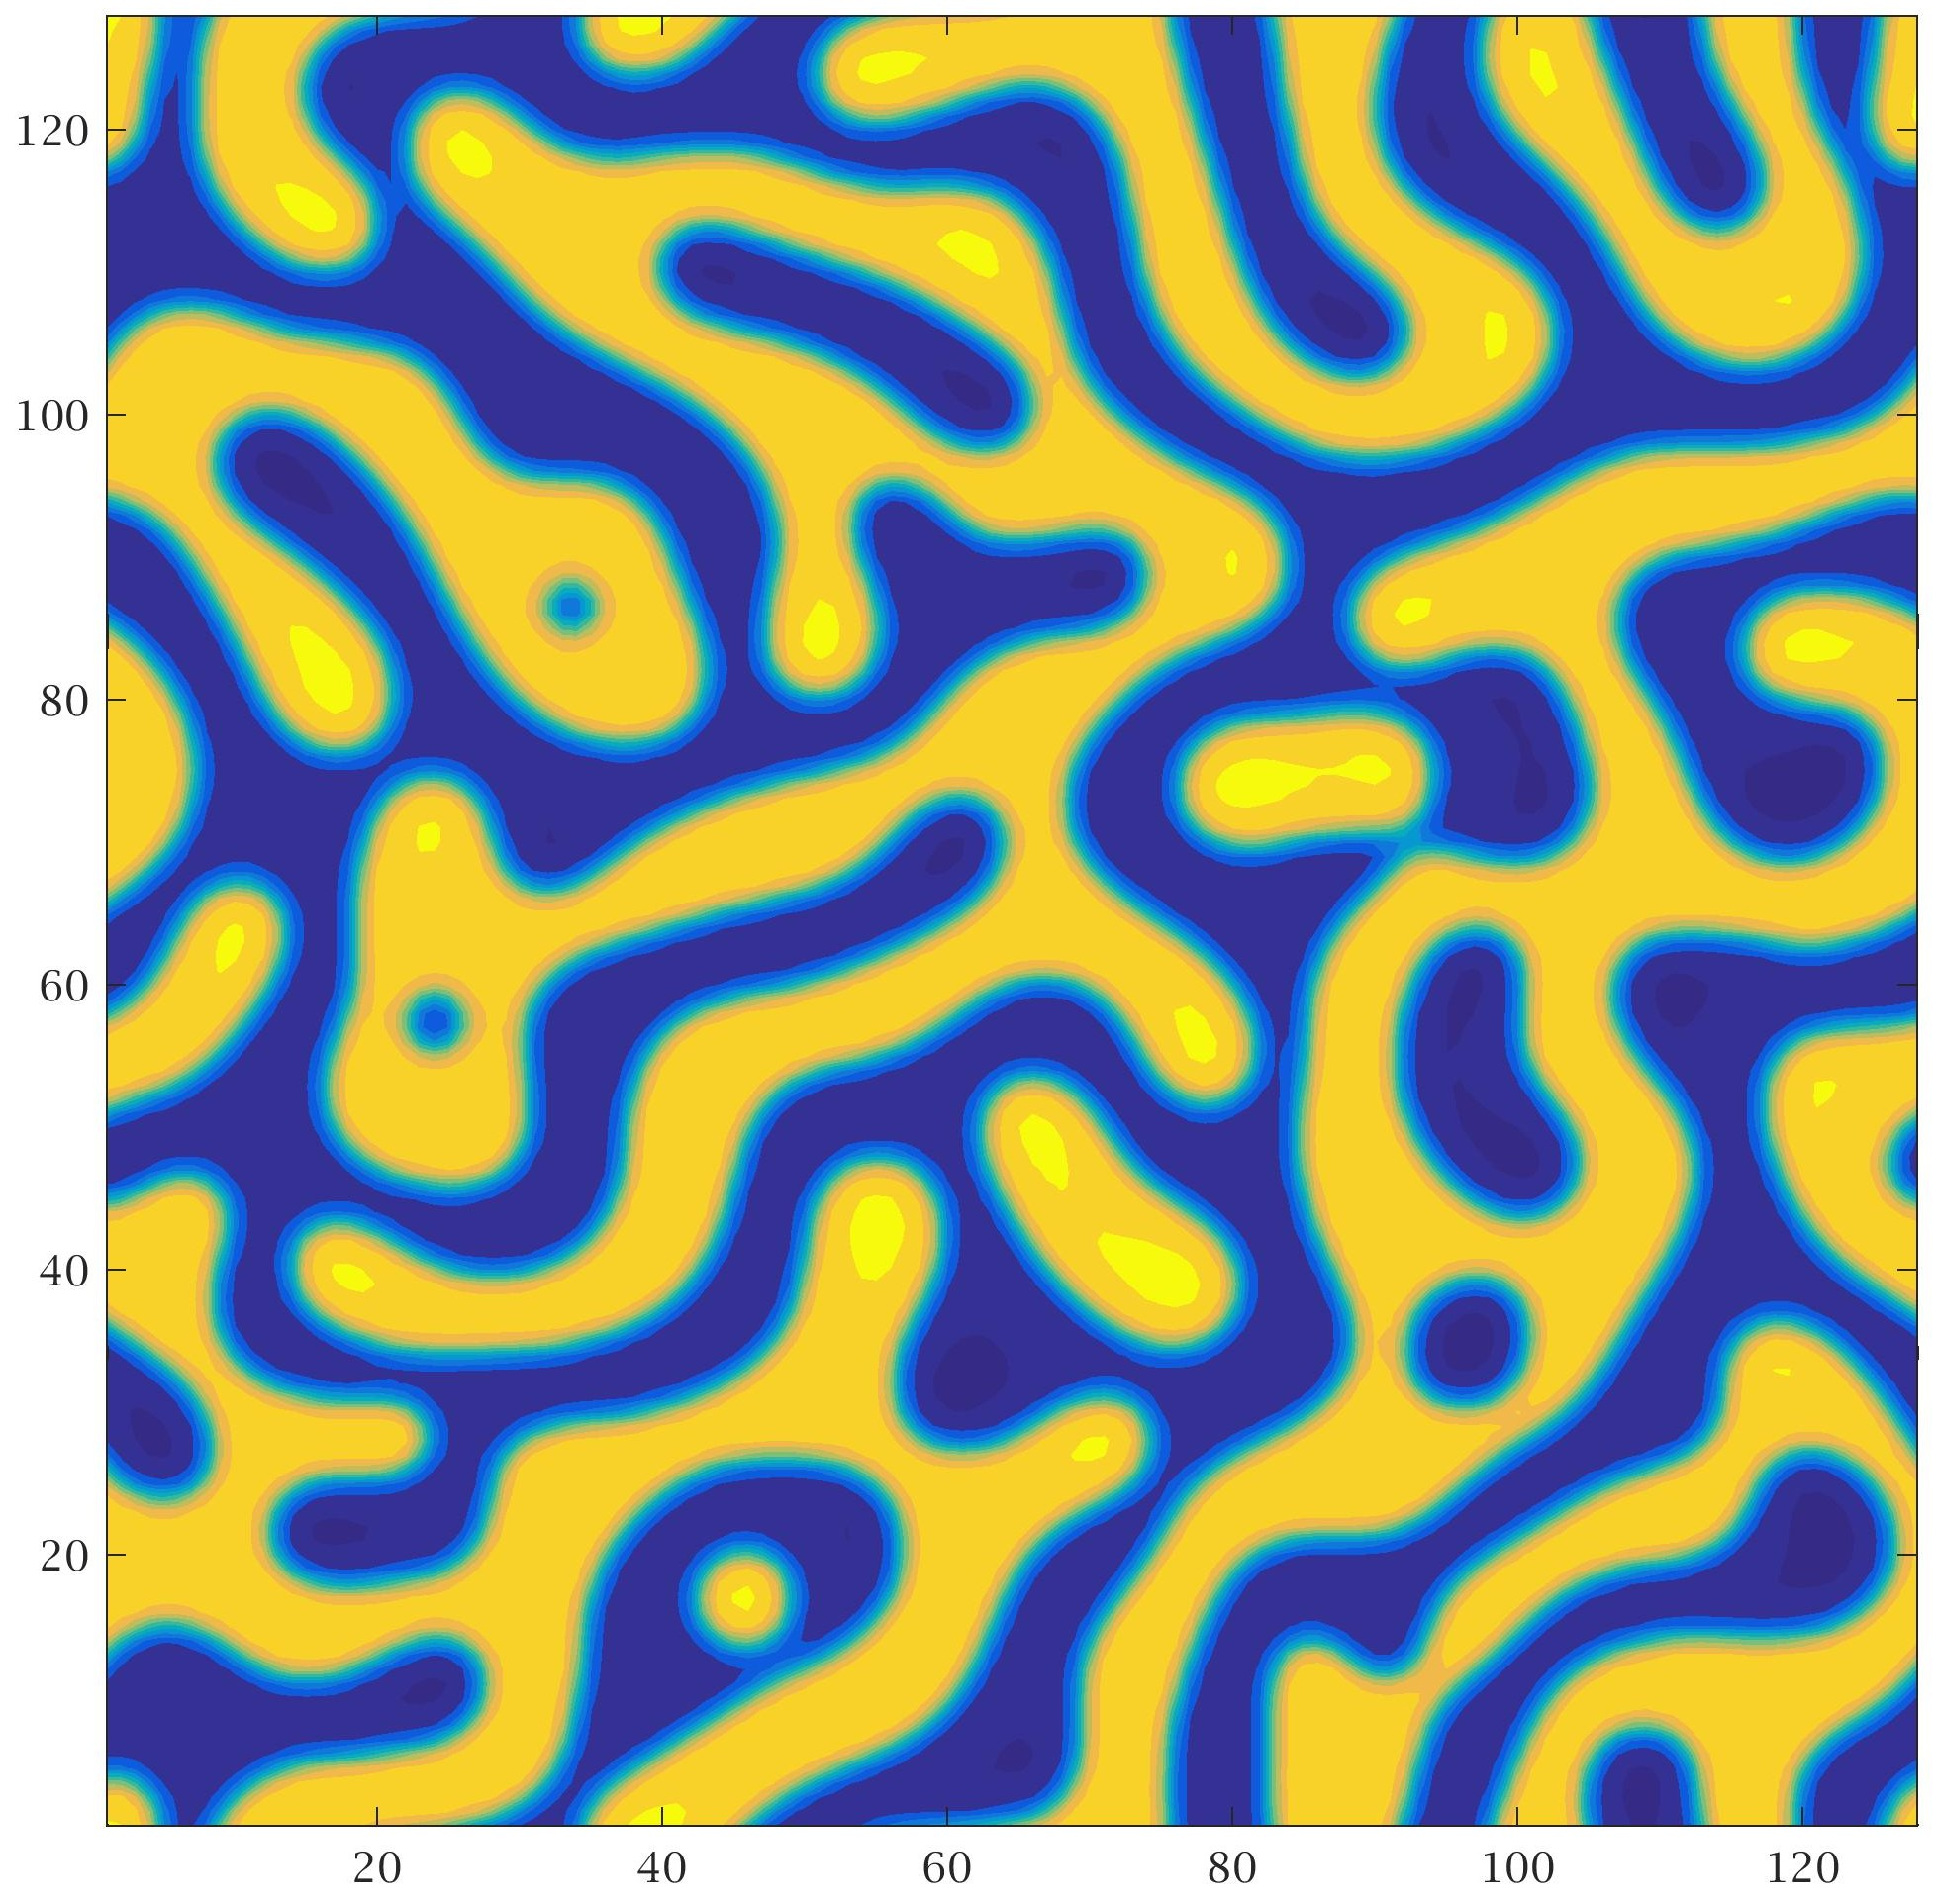
\includegraphics[width=1\textwidth]{pics/C2_t3.jpg}
                \subcaption{$t=10$}
        \end{minipage}
        
        \begin{minipage}[b]{.32\linewidth}        
                \centering
                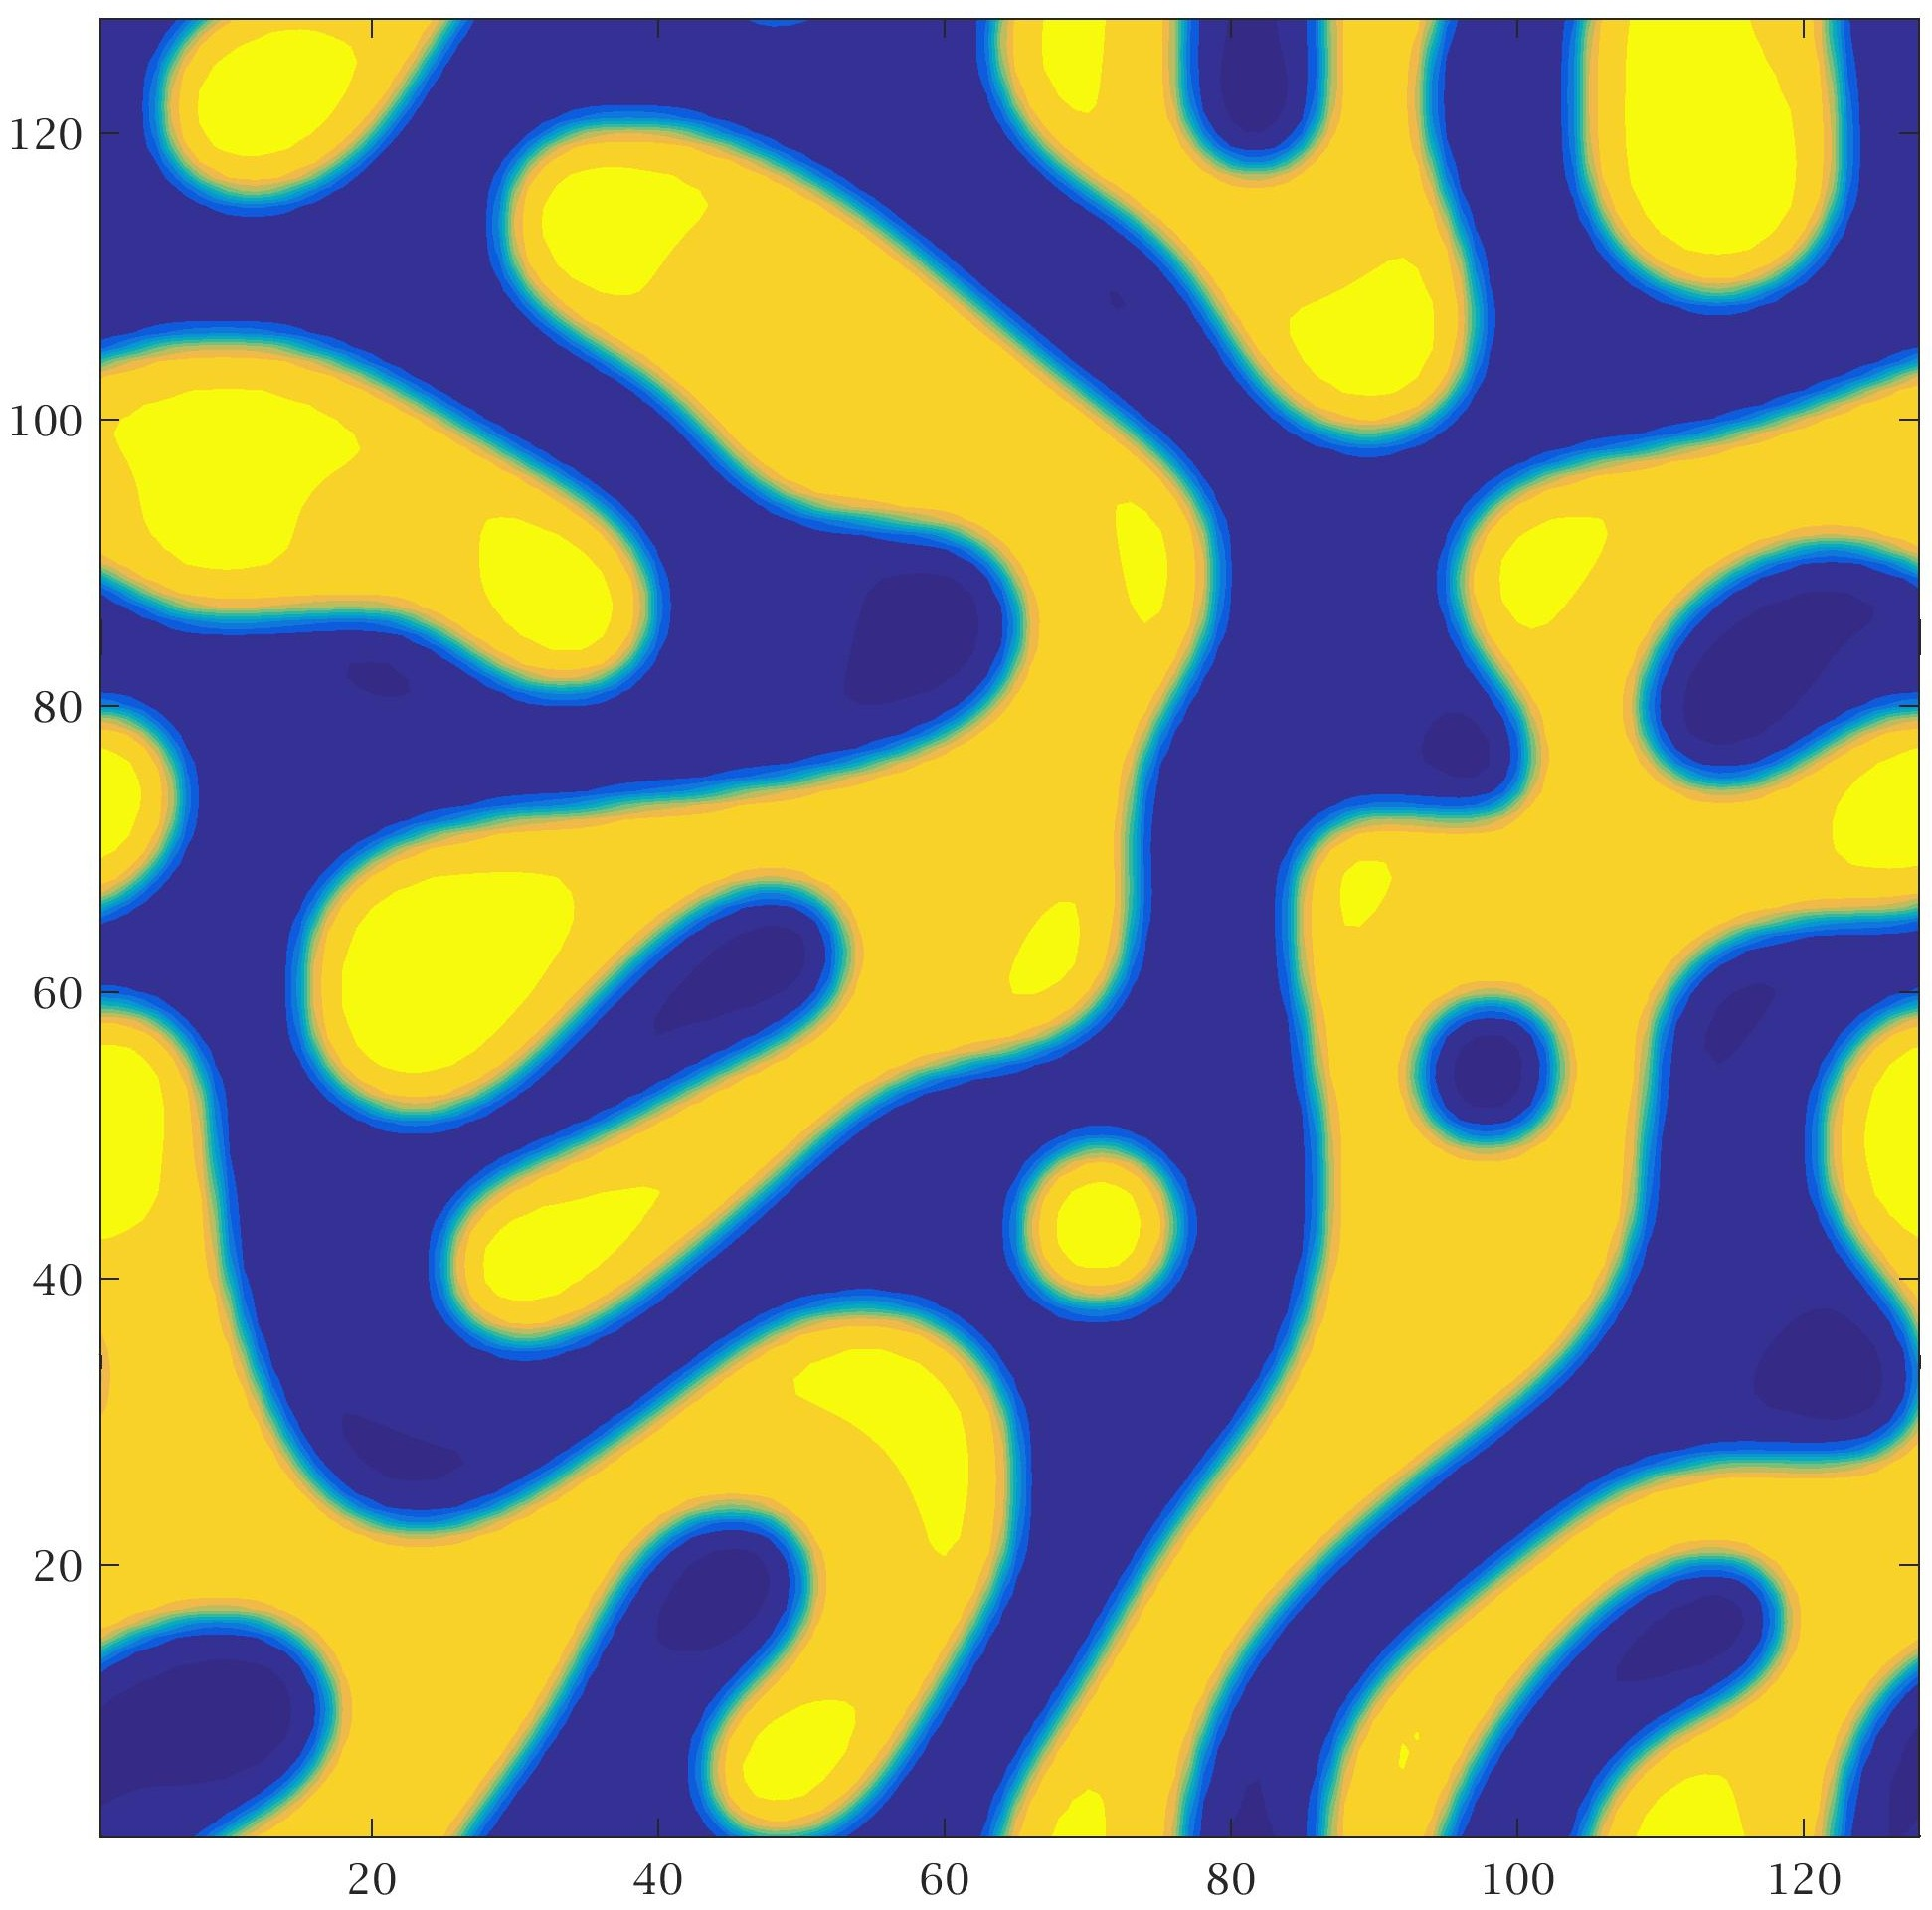
\includegraphics[width=1\textwidth]{pics/C2_t4.jpg}
                \subcaption{$t=50$}
        \end{minipage}
        %   \hfill
        \begin{minipage}[b]{.32\linewidth}
                \centering
                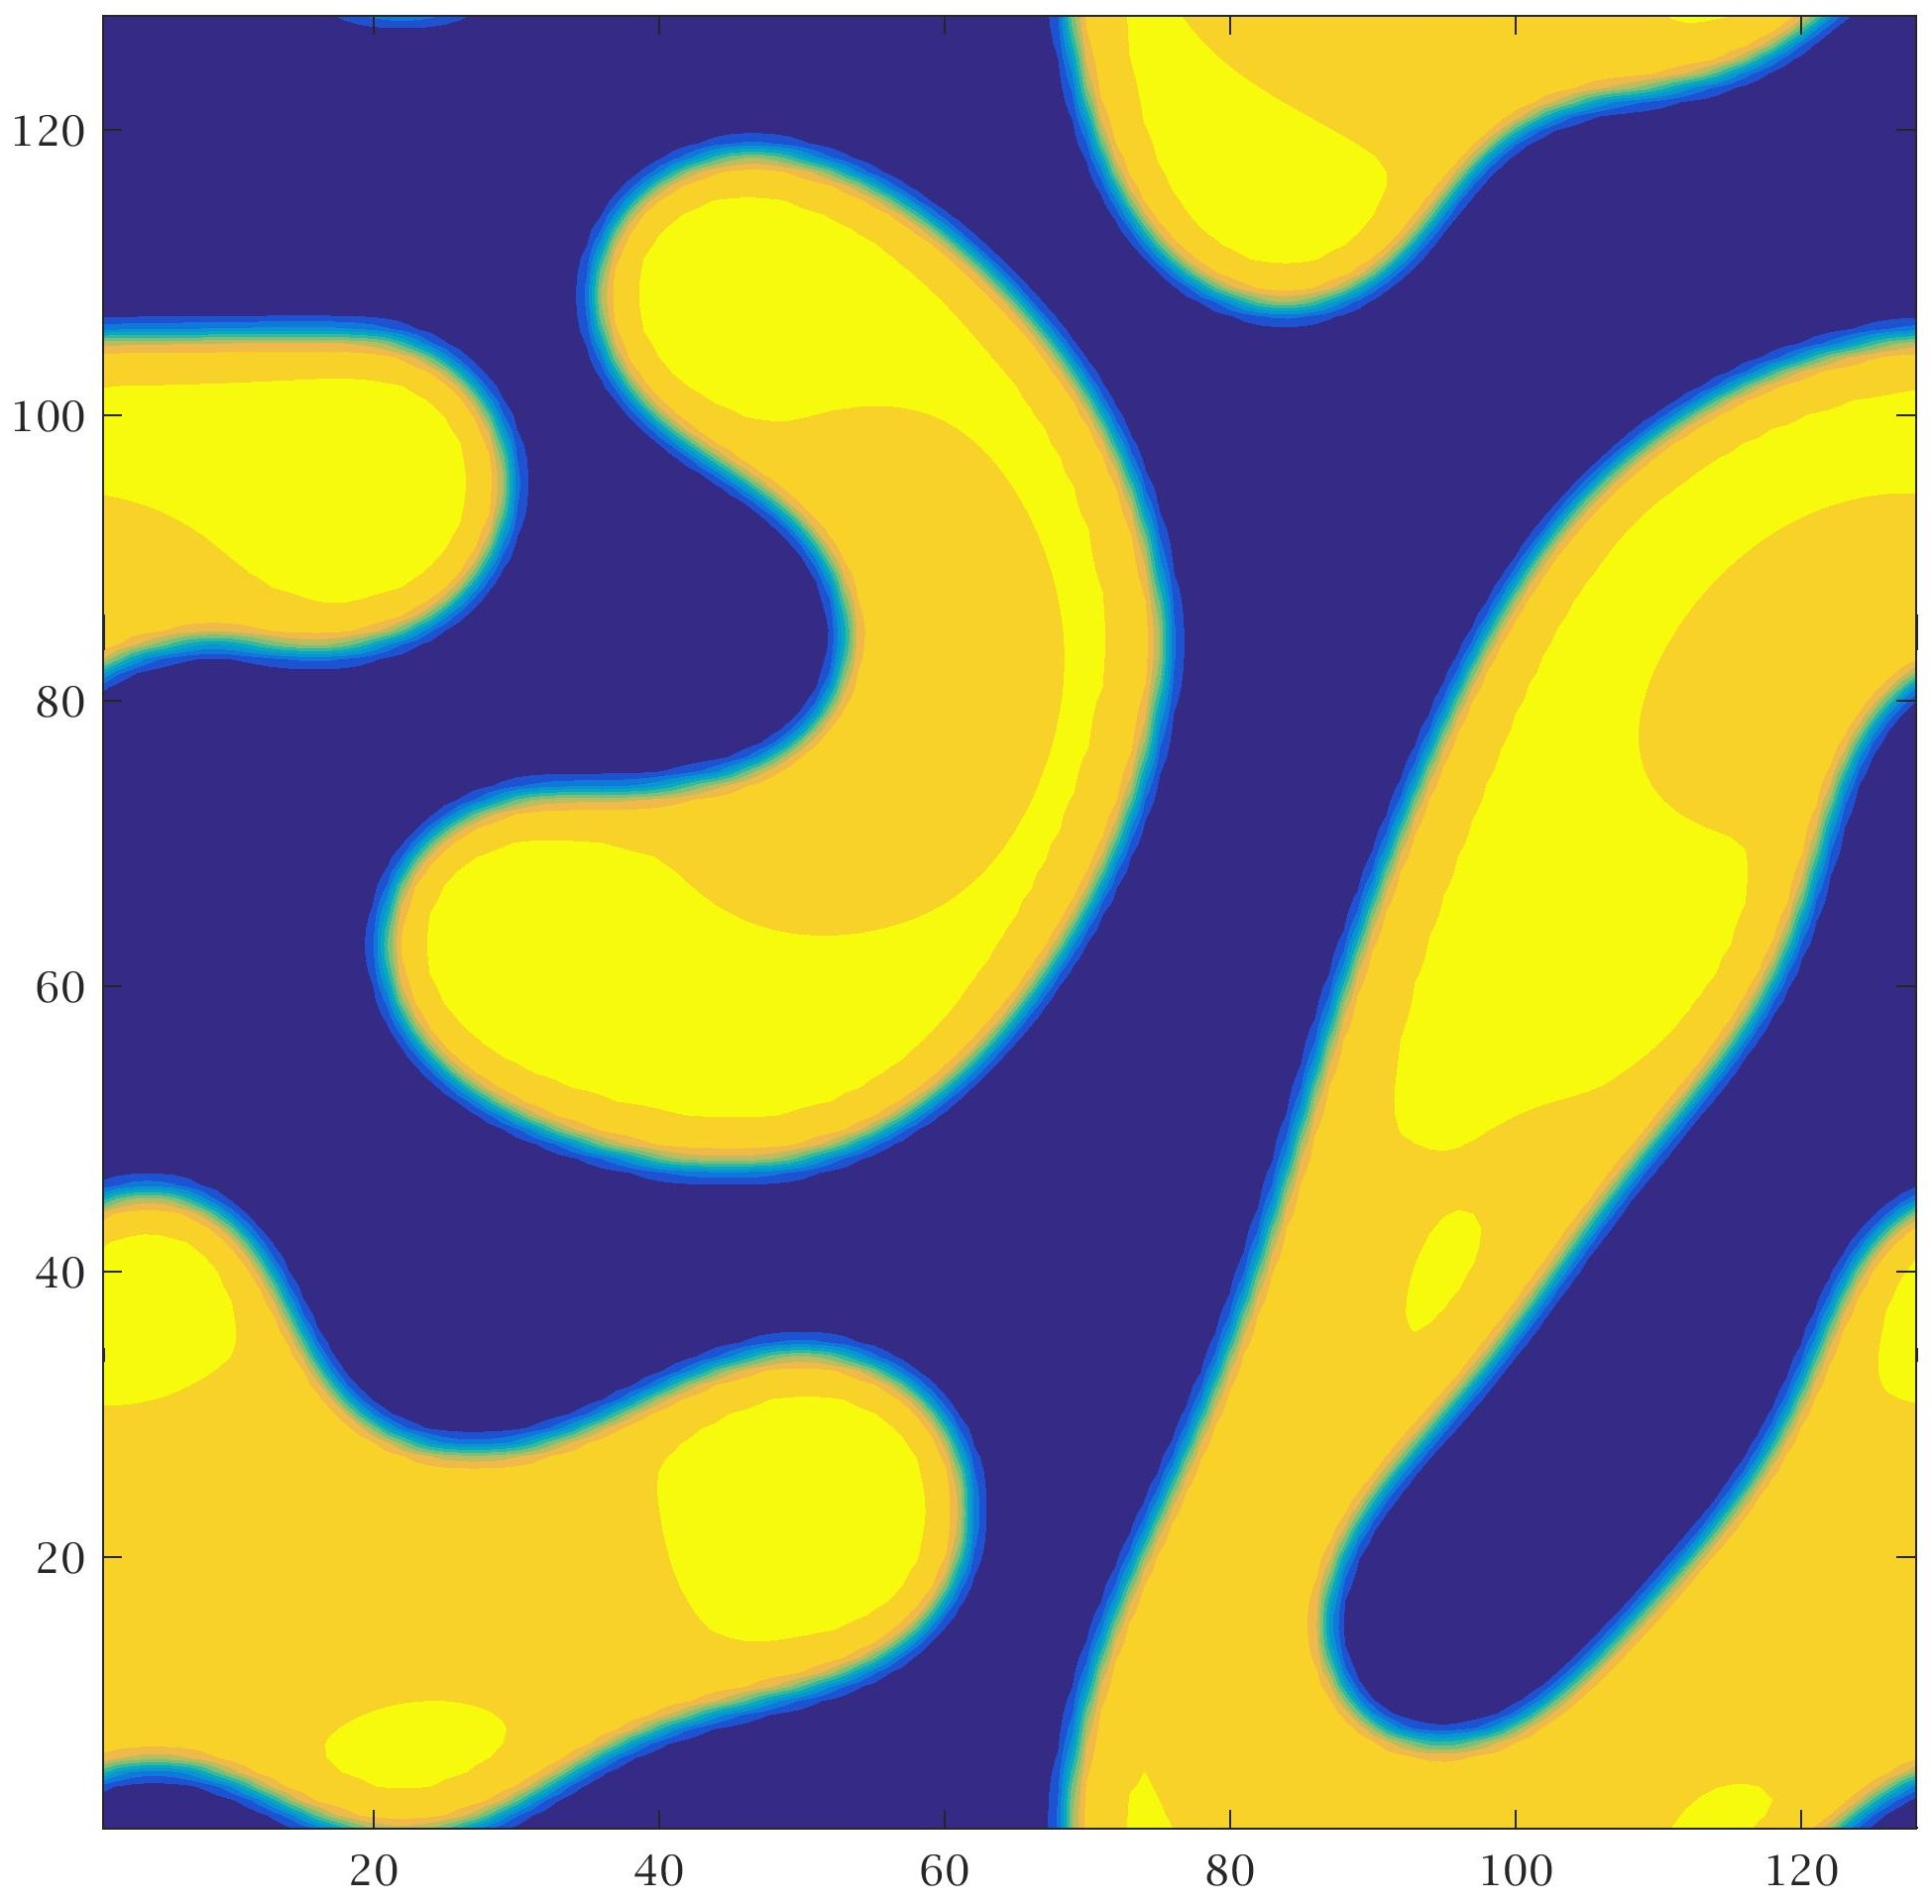
\includegraphics[width=1\textwidth]{pics/C2_t5.jpg}
                \subcaption{$t=200$}
        \end{minipage}
                \begin{minipage}[b]{.32\linewidth}
                \centering
                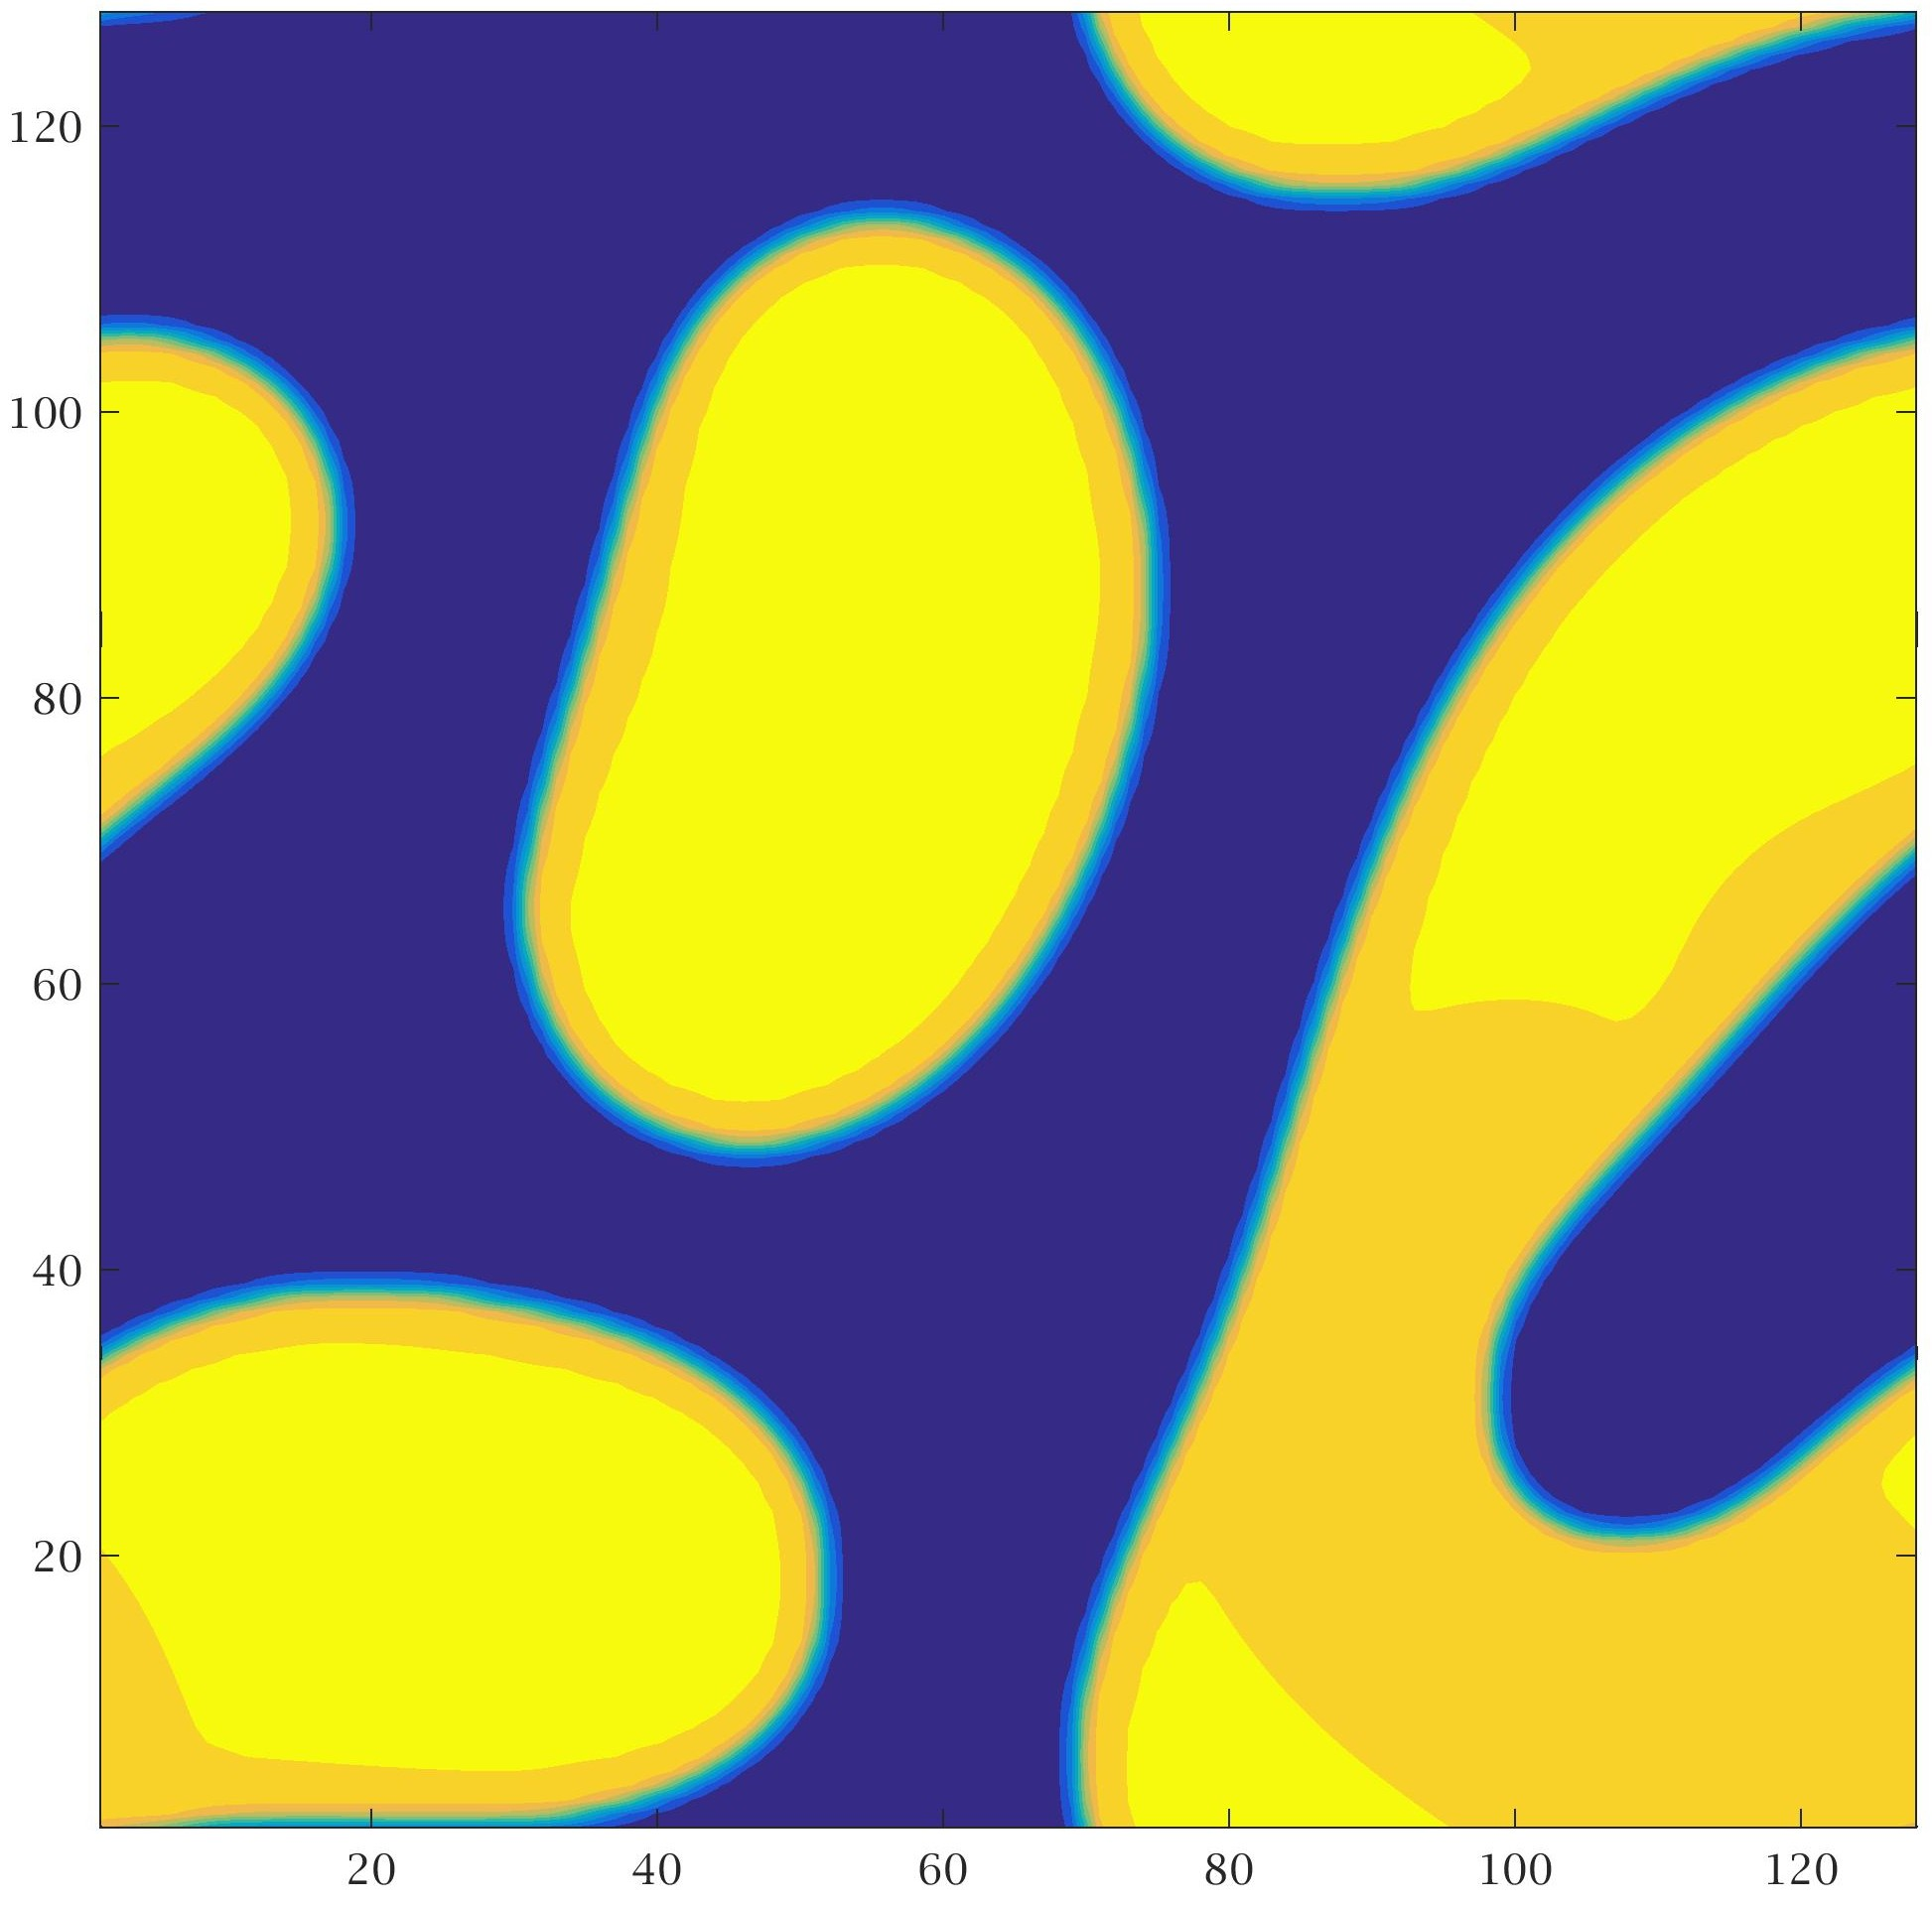
\includegraphics[width=1\textwidth]{pics/C2_t6.jpg}
                \subcaption{$t=500$}
        \end{minipage}
        \caption{Evolution with the average concentration of 0.5}
        \label{evolution_c2}
\end{figure}

Figures (\ref{E_c2} \& \ref{L_c2}) also shows the energy and characteristic length as the function of time for three different runs with the average concentration on 0.5.

Figure (\ref{E_c2}) demonstrates that the energy decreases at a rate between $t^{-1/4}$ and $t^{-1/3}$; however, figure (\ref{L_c2}) shows that the characteristic length grows at a rate between $t^{1/4}$ and $t^{1/3}$.

\begin{figure}[H]
        \begin{minipage}[b]{.5\linewidth}        
                \centering
                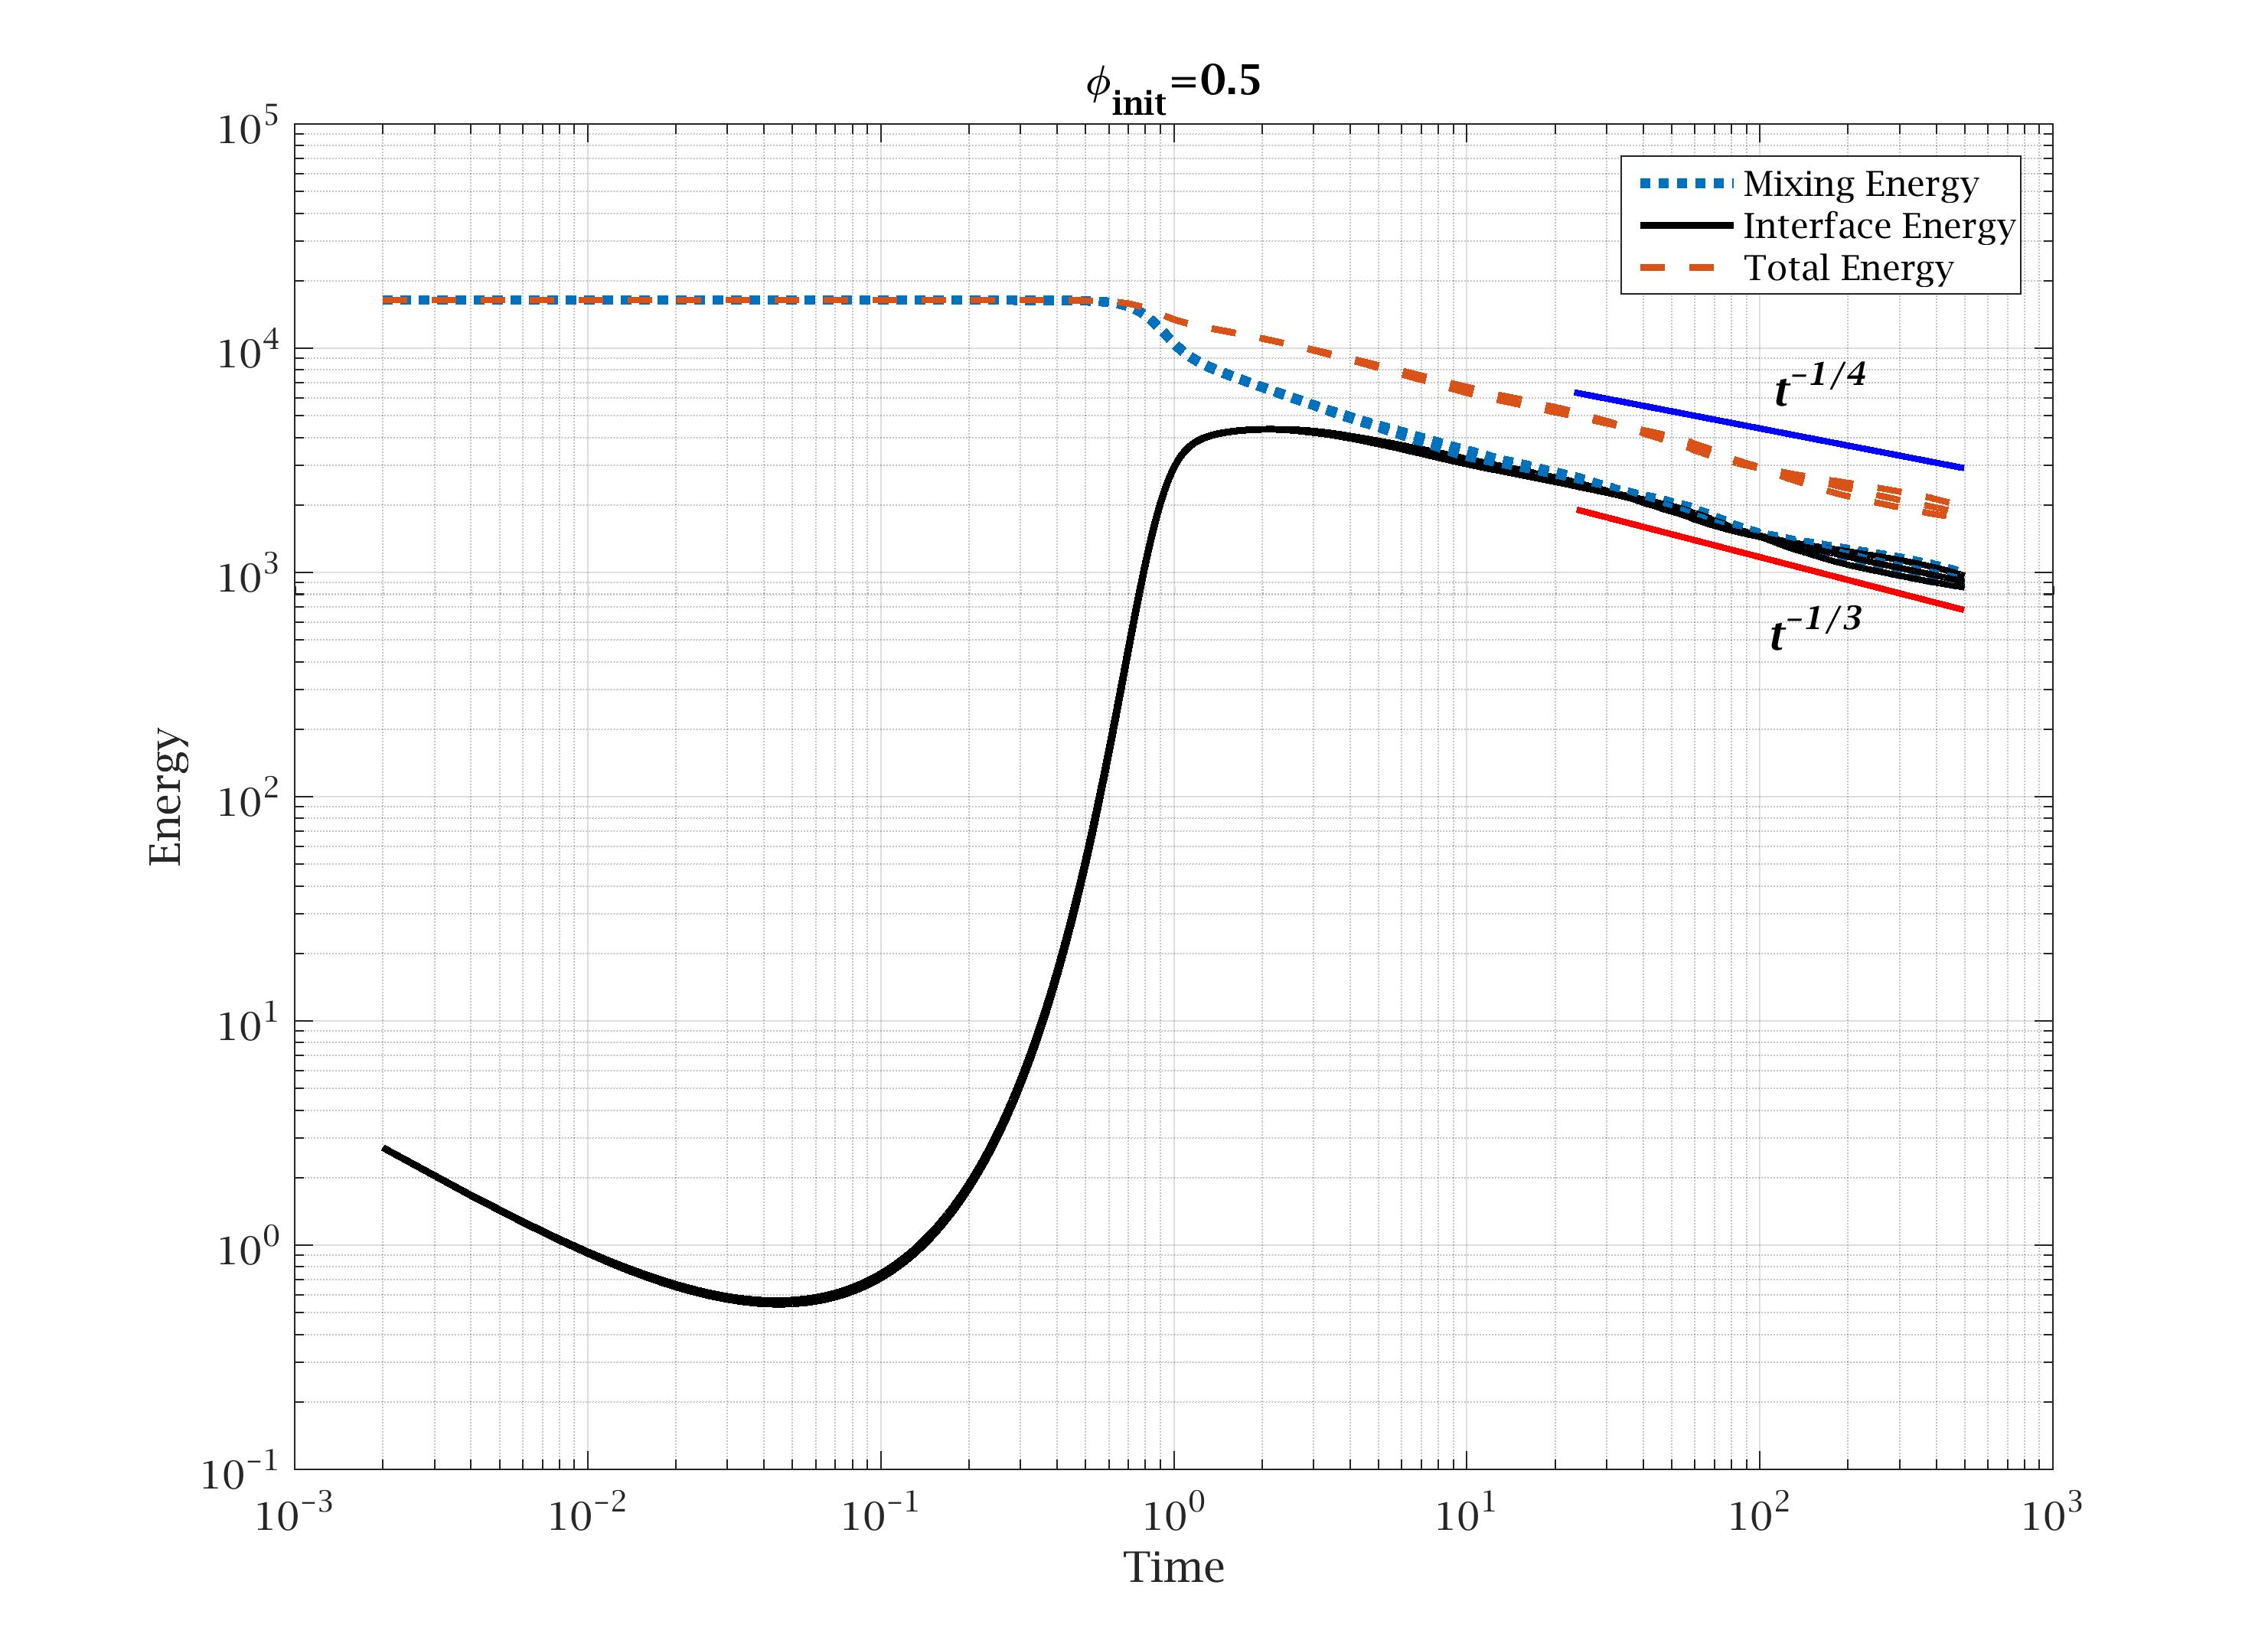
\includegraphics[width=1\textwidth]{pics/E_c2.jpg}
                \subcaption{}
				\label{E_c2}
        \end{minipage}
        %   \hfill
        \begin{minipage}[b]{.5\linewidth}
                \centering
                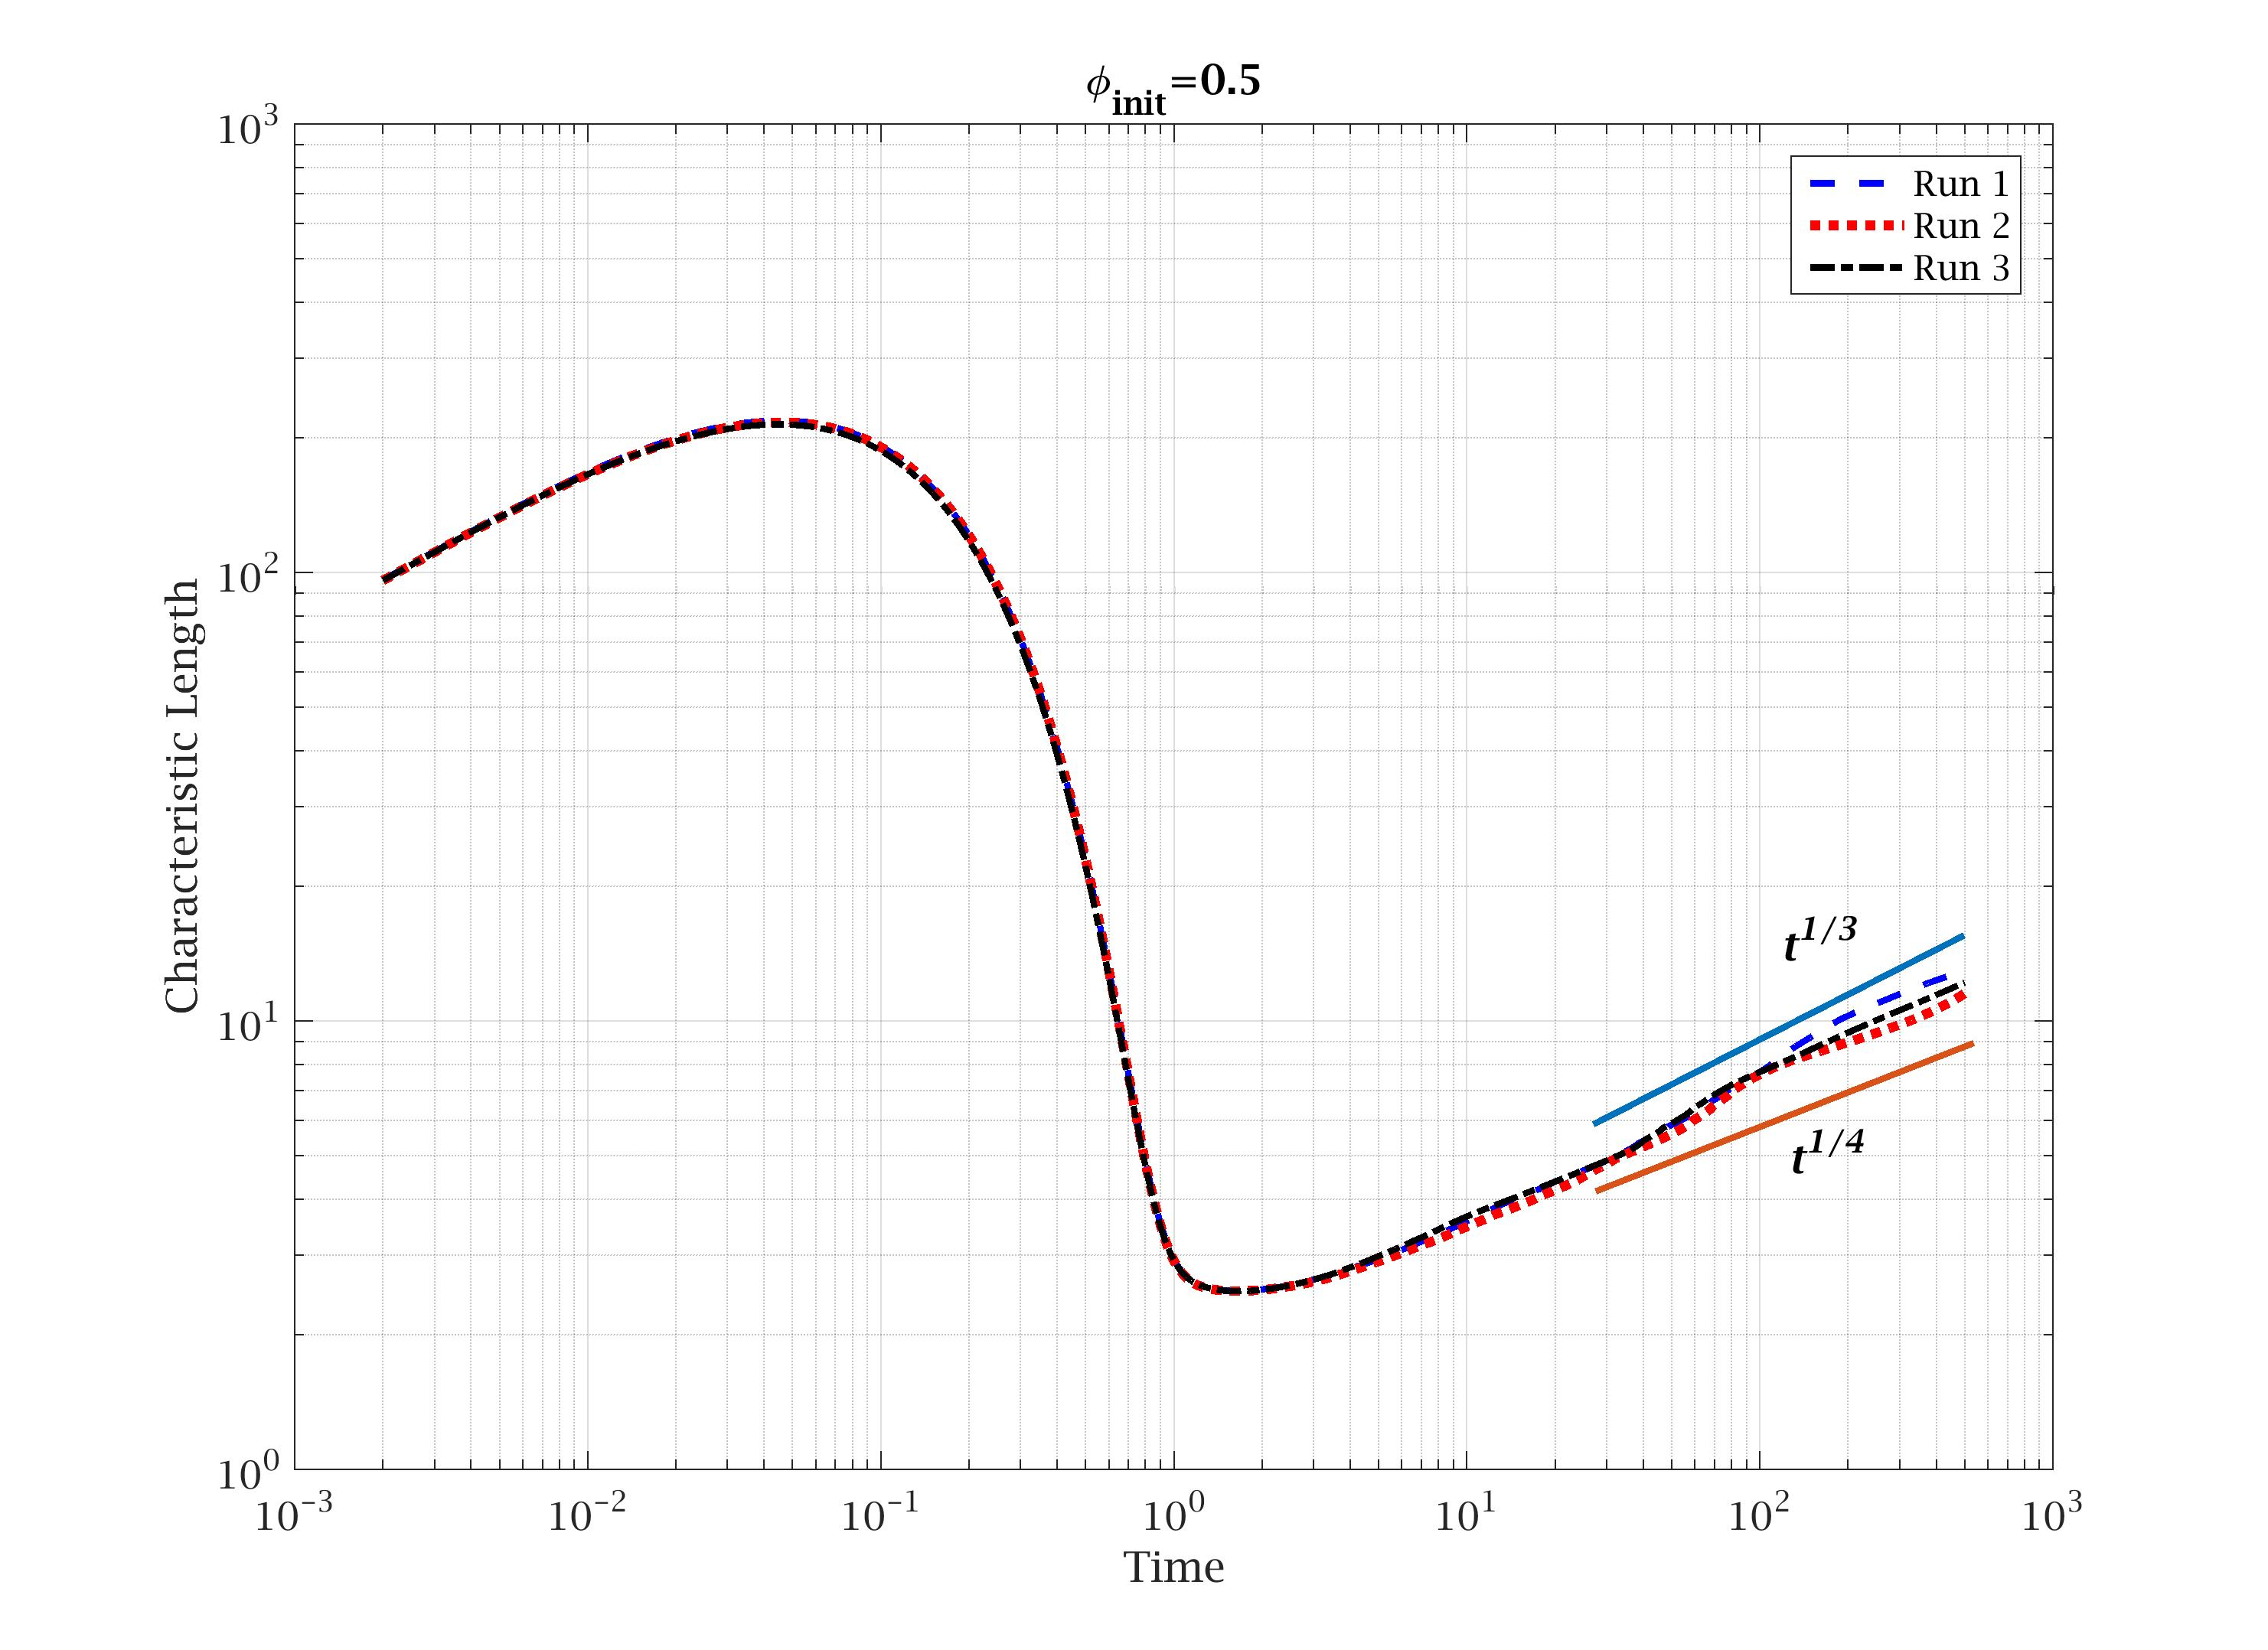
\includegraphics[width=1\textwidth]{pics/L_c2.jpg}
                \subcaption{}
                	\label{L_c2}
        \end{minipage}
                \caption{The (a) interfacial, mixing and total energy and (b) characteristic length as a function of time for the average concentration of 0.5}
        \label{EL_c2}
\end{figure}

\subsection{Case 3, Ave. concentration of 0.7}

Here the figure (\ref{evolution_c3}) shows the evolution of the phase filed variable for the average concentration of 0.7.
\begin{figure}[H]
        \begin{minipage}[b]{.32\linewidth}        
                \centering
                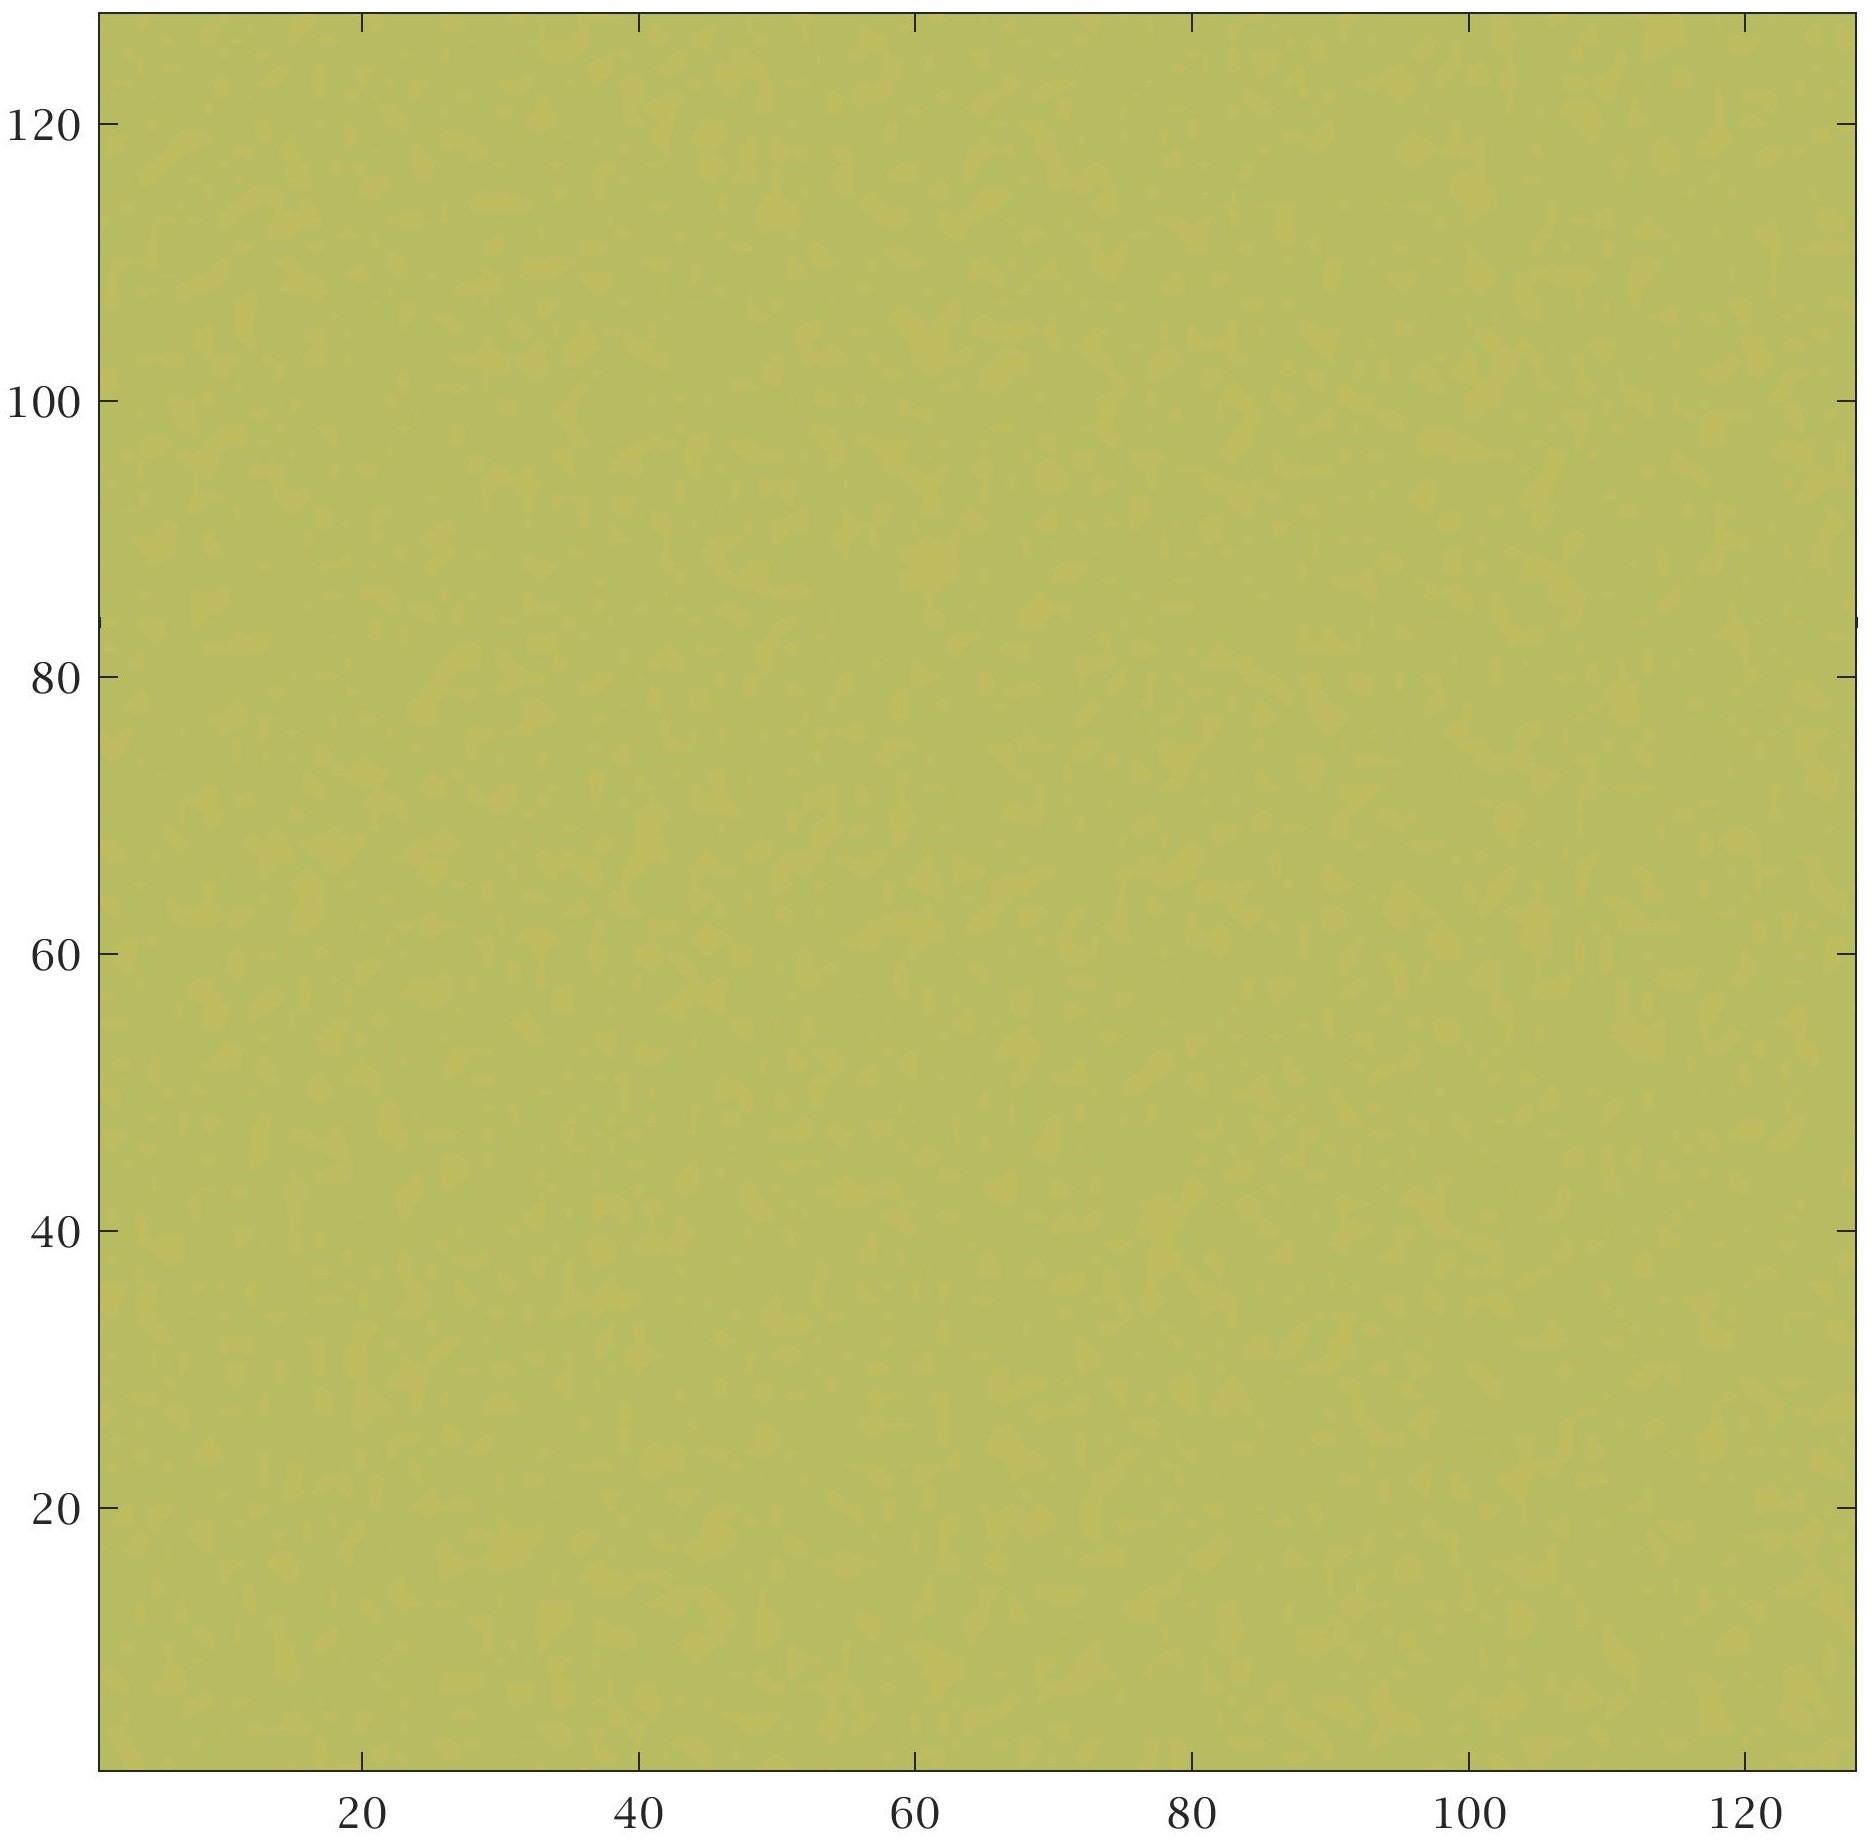
\includegraphics[width=1\textwidth]{pics/C3_t1.jpg}
                \subcaption{$t=0$}
        \end{minipage}
        %   \hfill
        \begin{minipage}[b]{.32\linewidth}
                \centering
                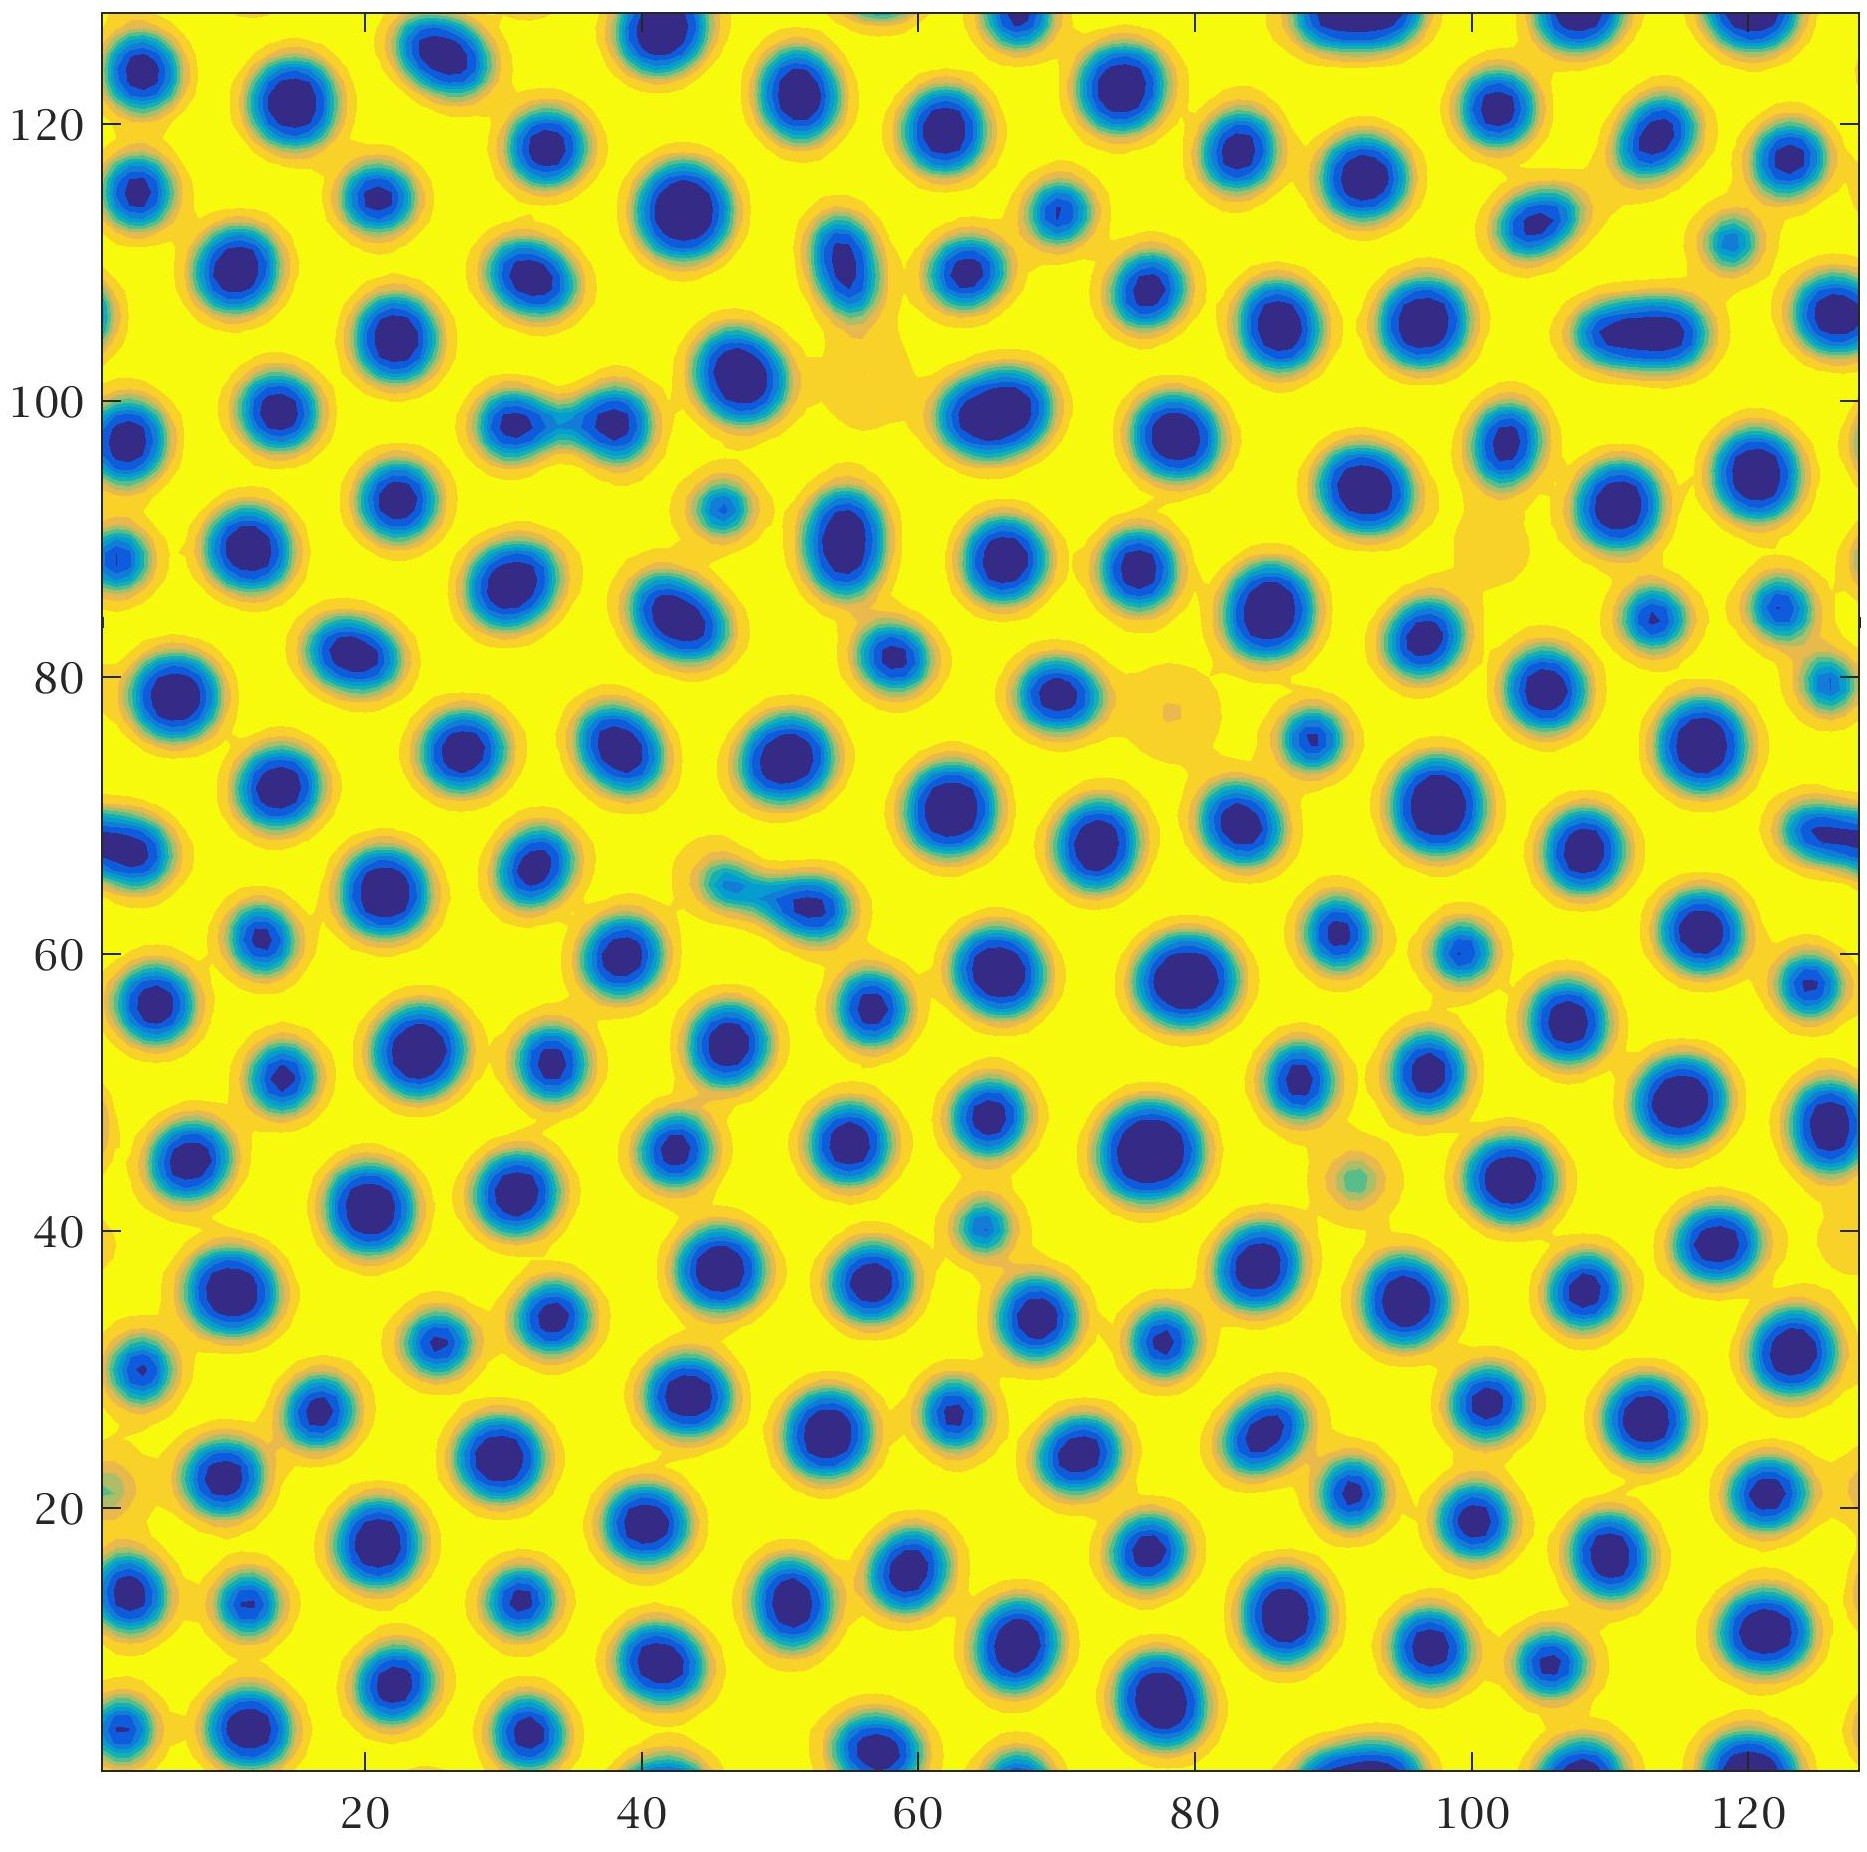
\includegraphics[width=1\textwidth]{pics/C3_t2.jpg}
                \subcaption{$t=4$}
        \end{minipage}
                \begin{minipage}[b]{.32\linewidth}
                \centering
                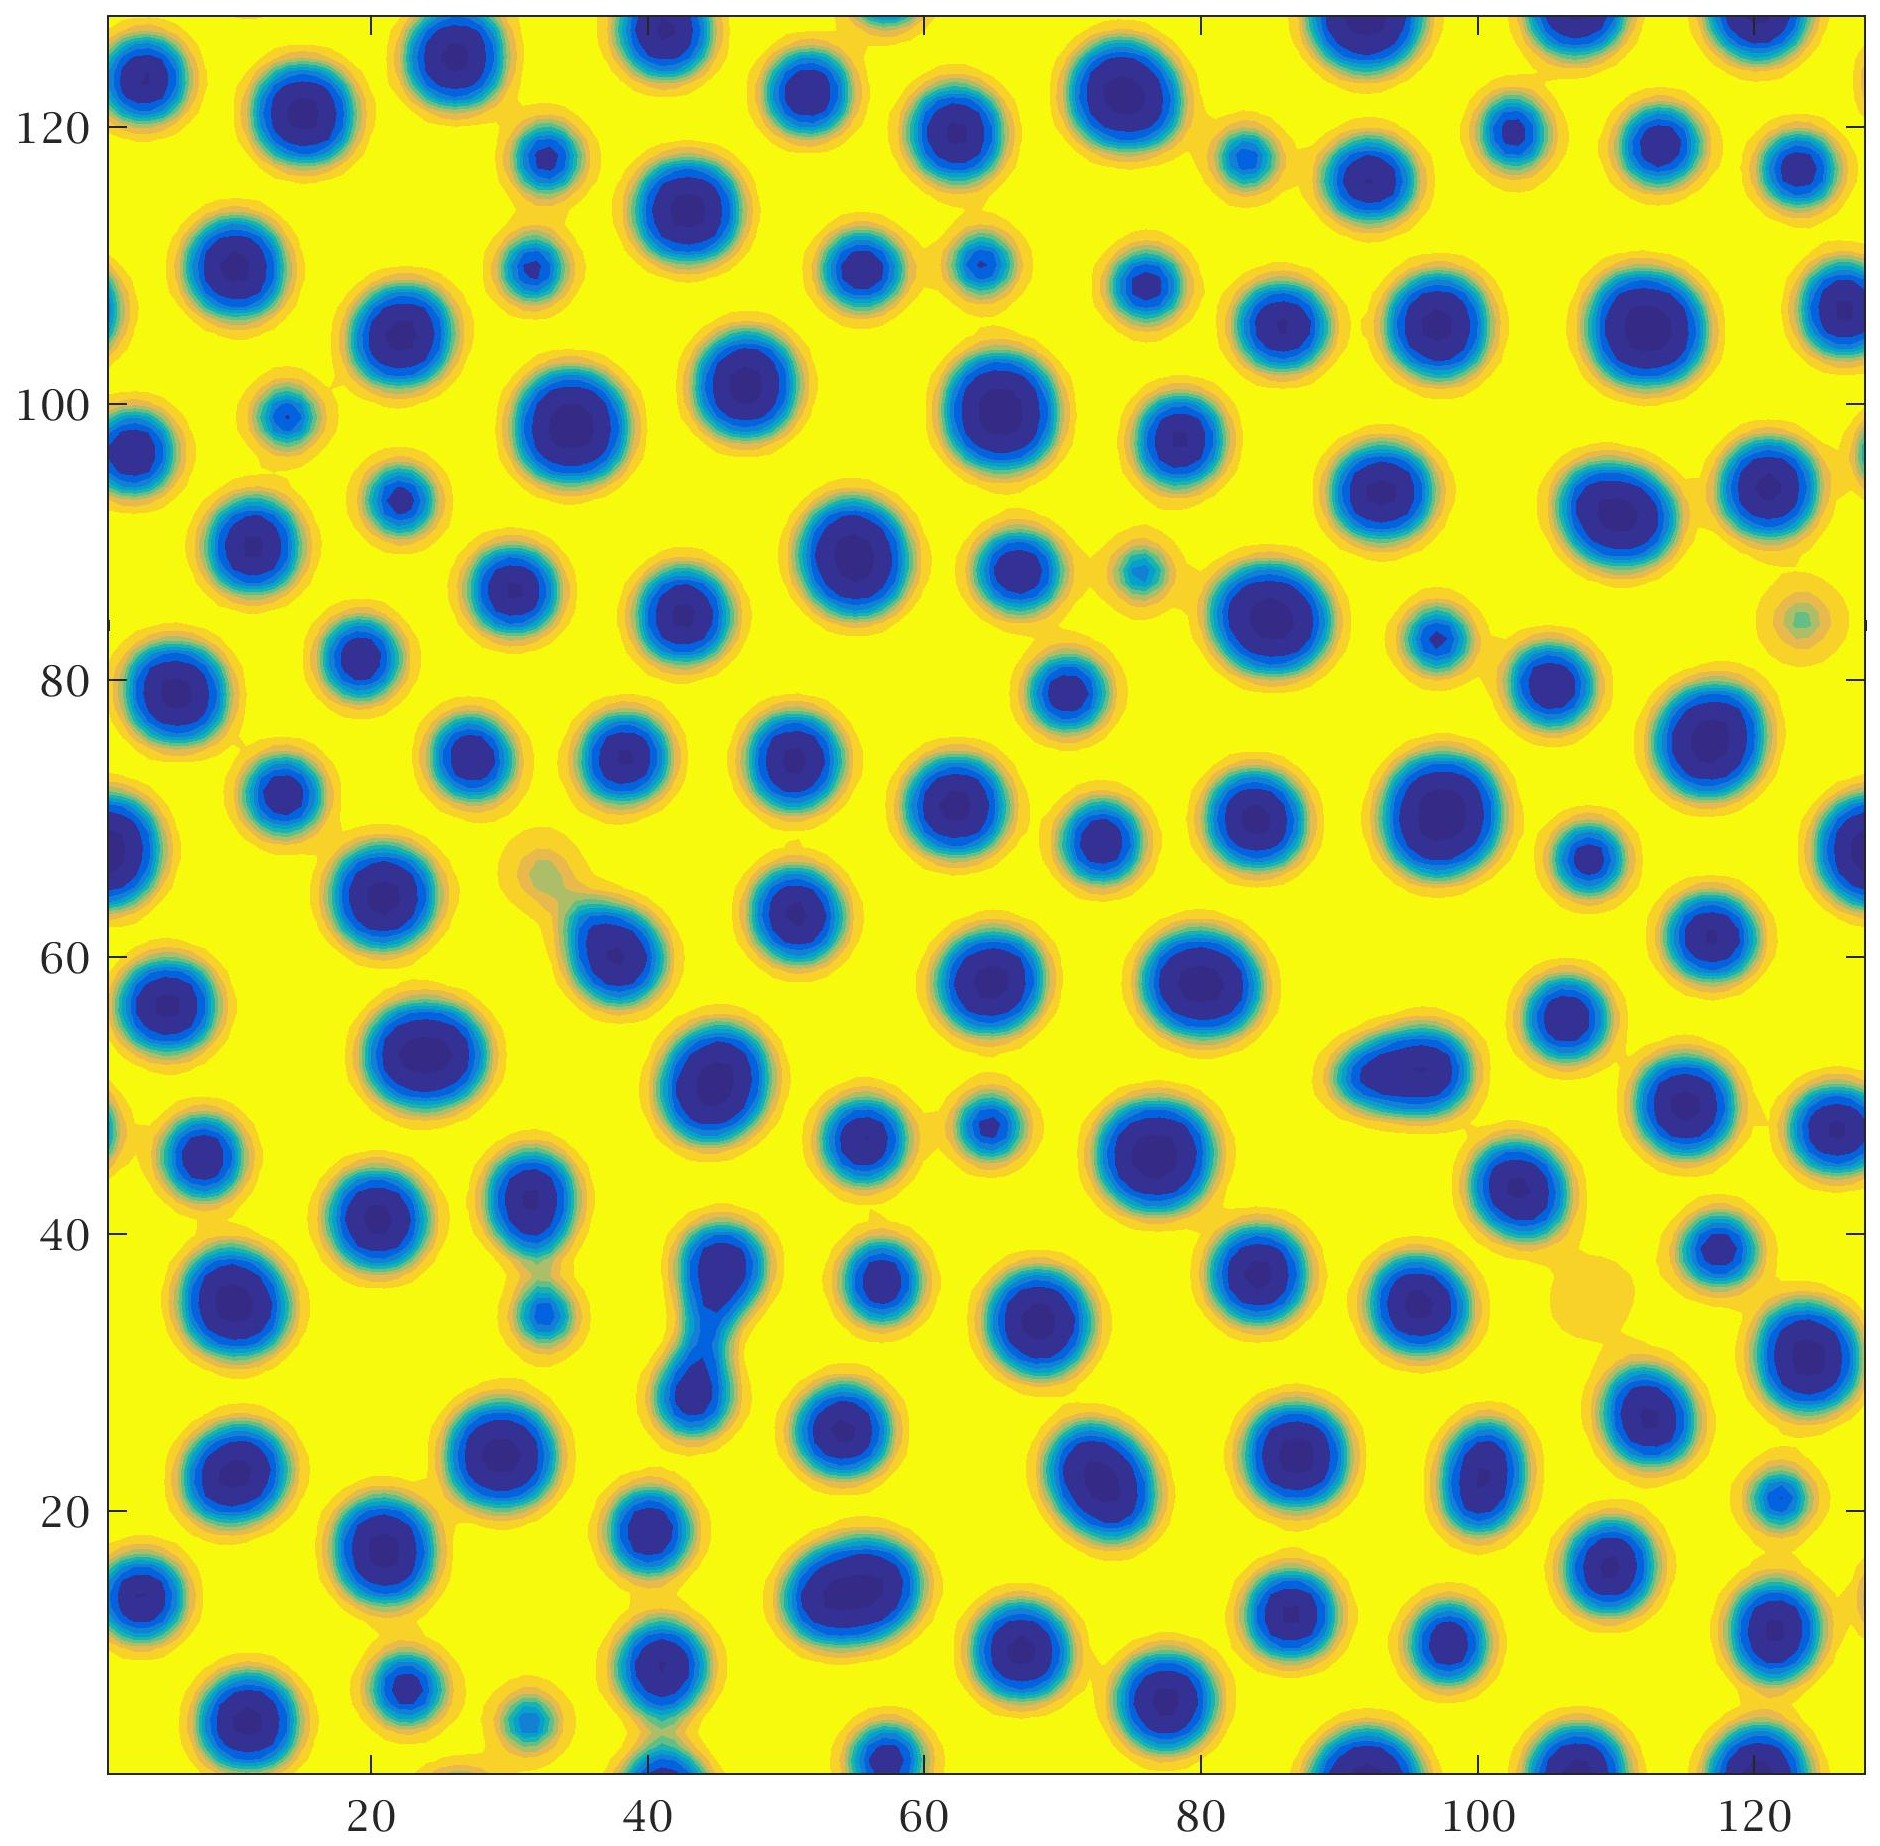
\includegraphics[width=1\textwidth]{pics/C3_t3.jpg}
                \subcaption{$t=10$}
        \end{minipage}
        
        \begin{minipage}[b]{.32\linewidth}        
                \centering
                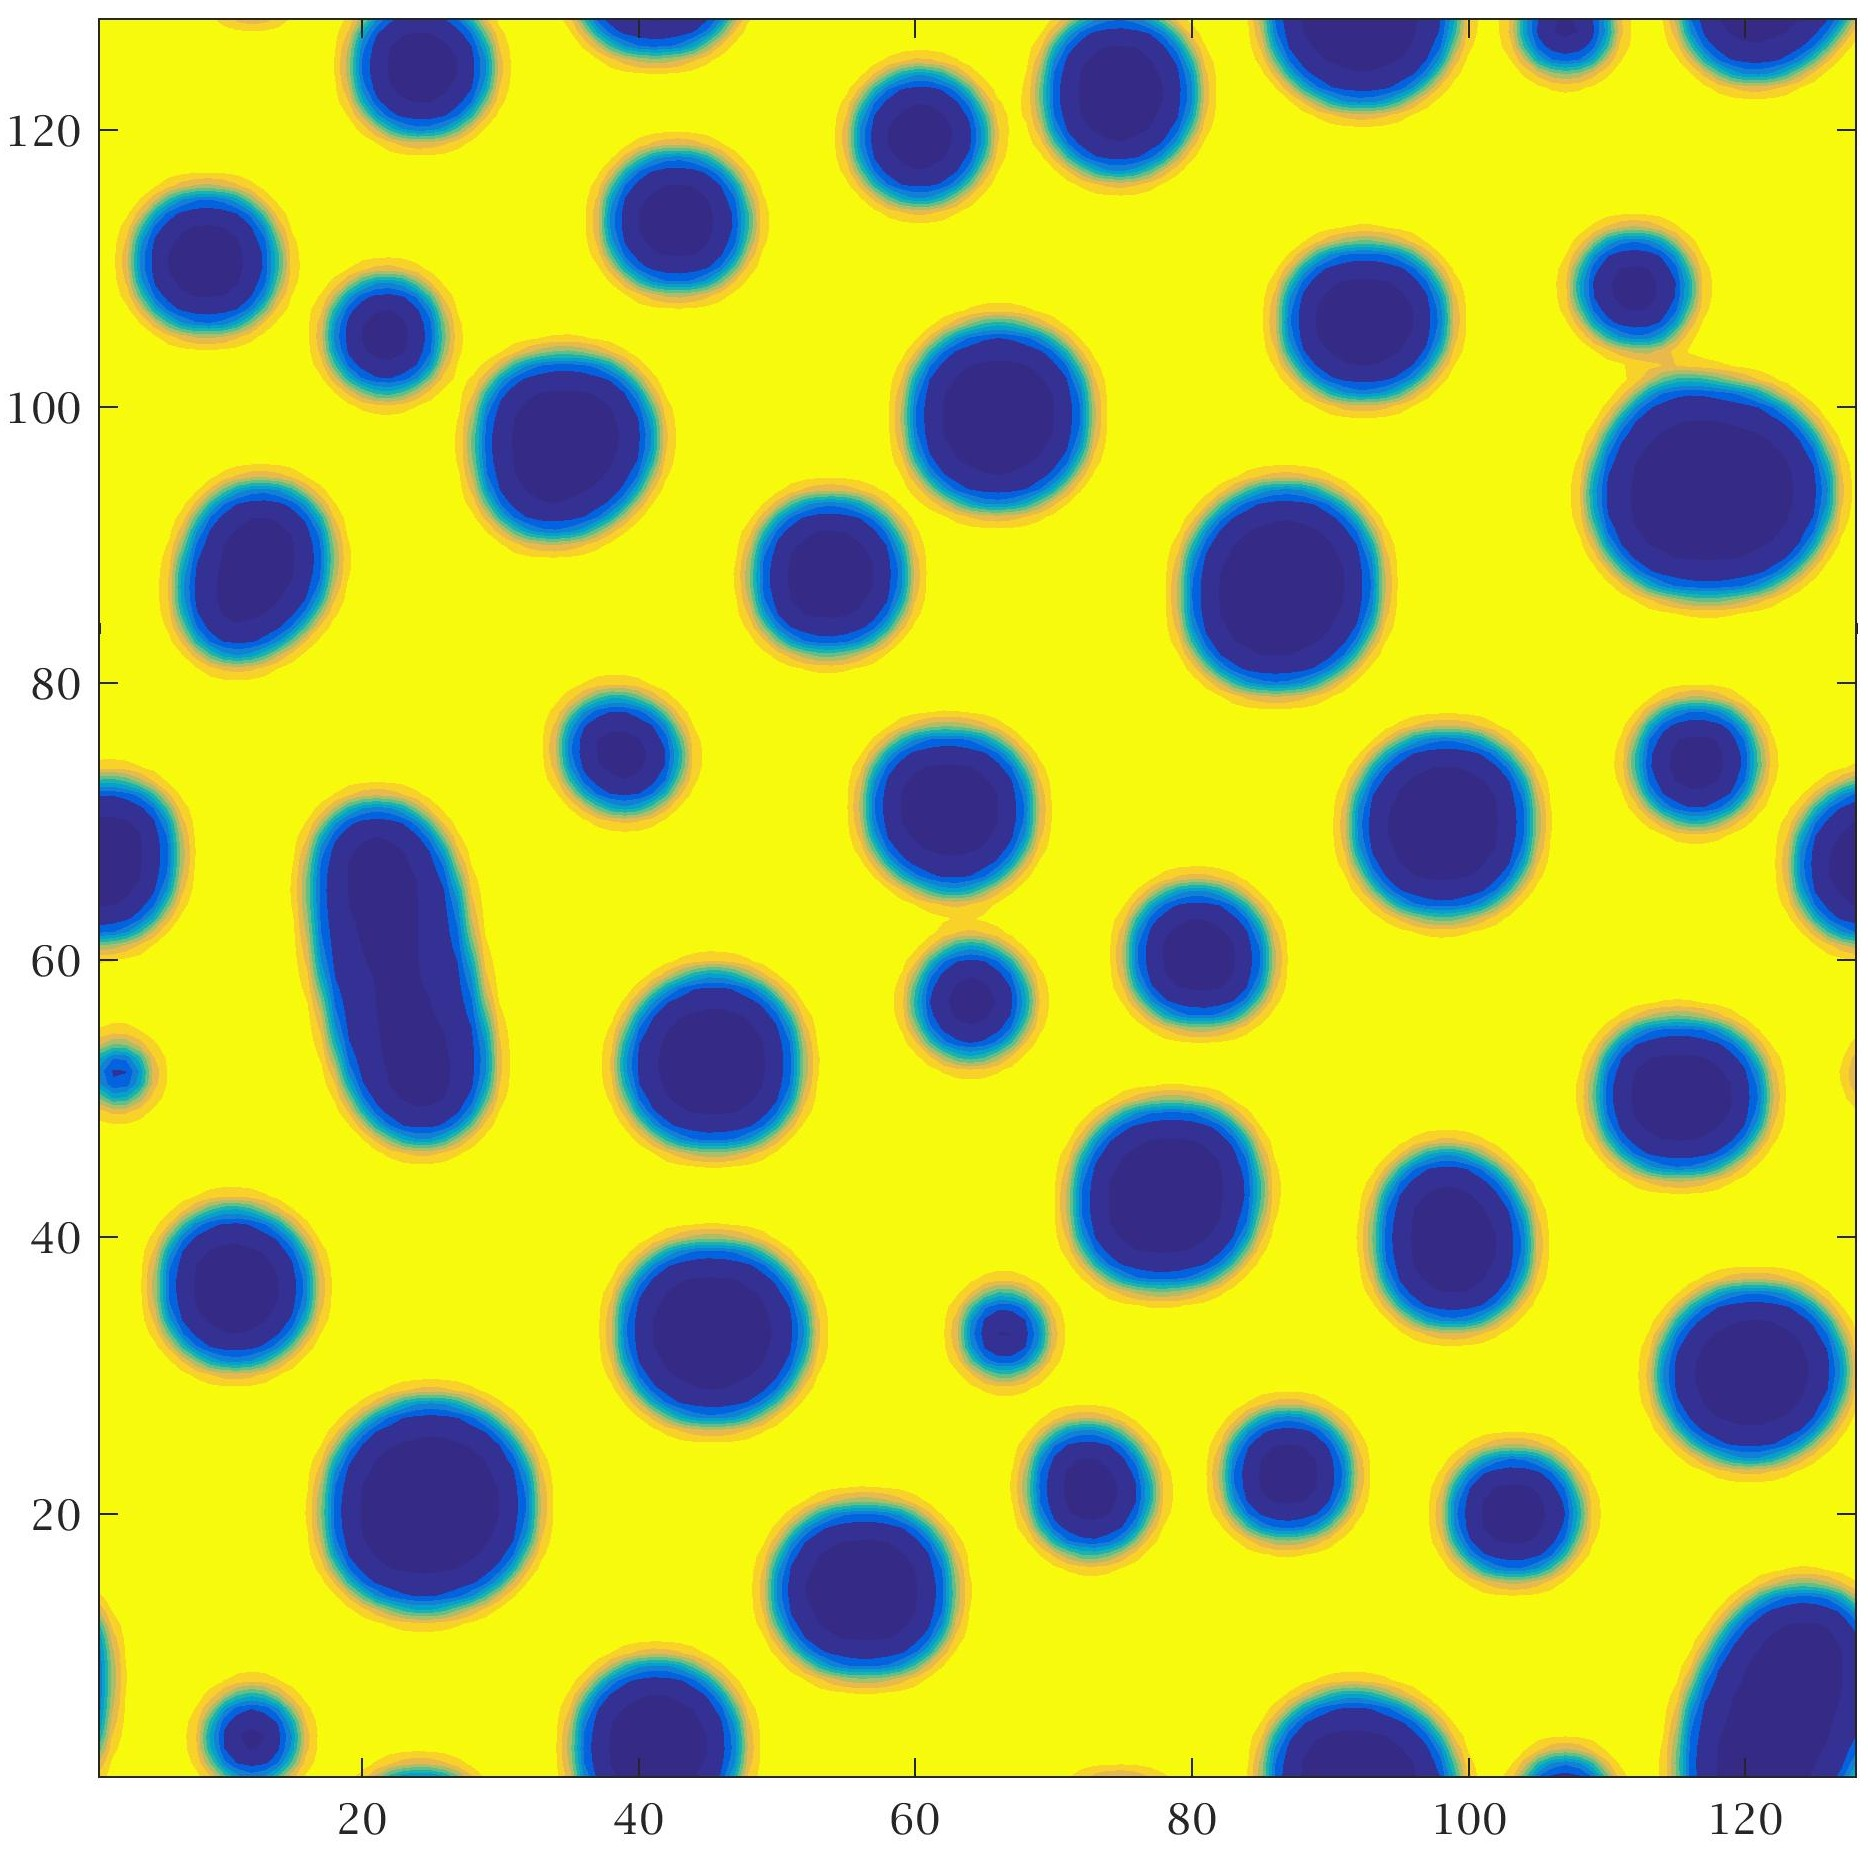
\includegraphics[width=1\textwidth]{pics/C3_t4.jpg}
                \subcaption{$t=50$}
        \end{minipage}
        %   \hfill
        \begin{minipage}[b]{.32\linewidth}
                \centering
                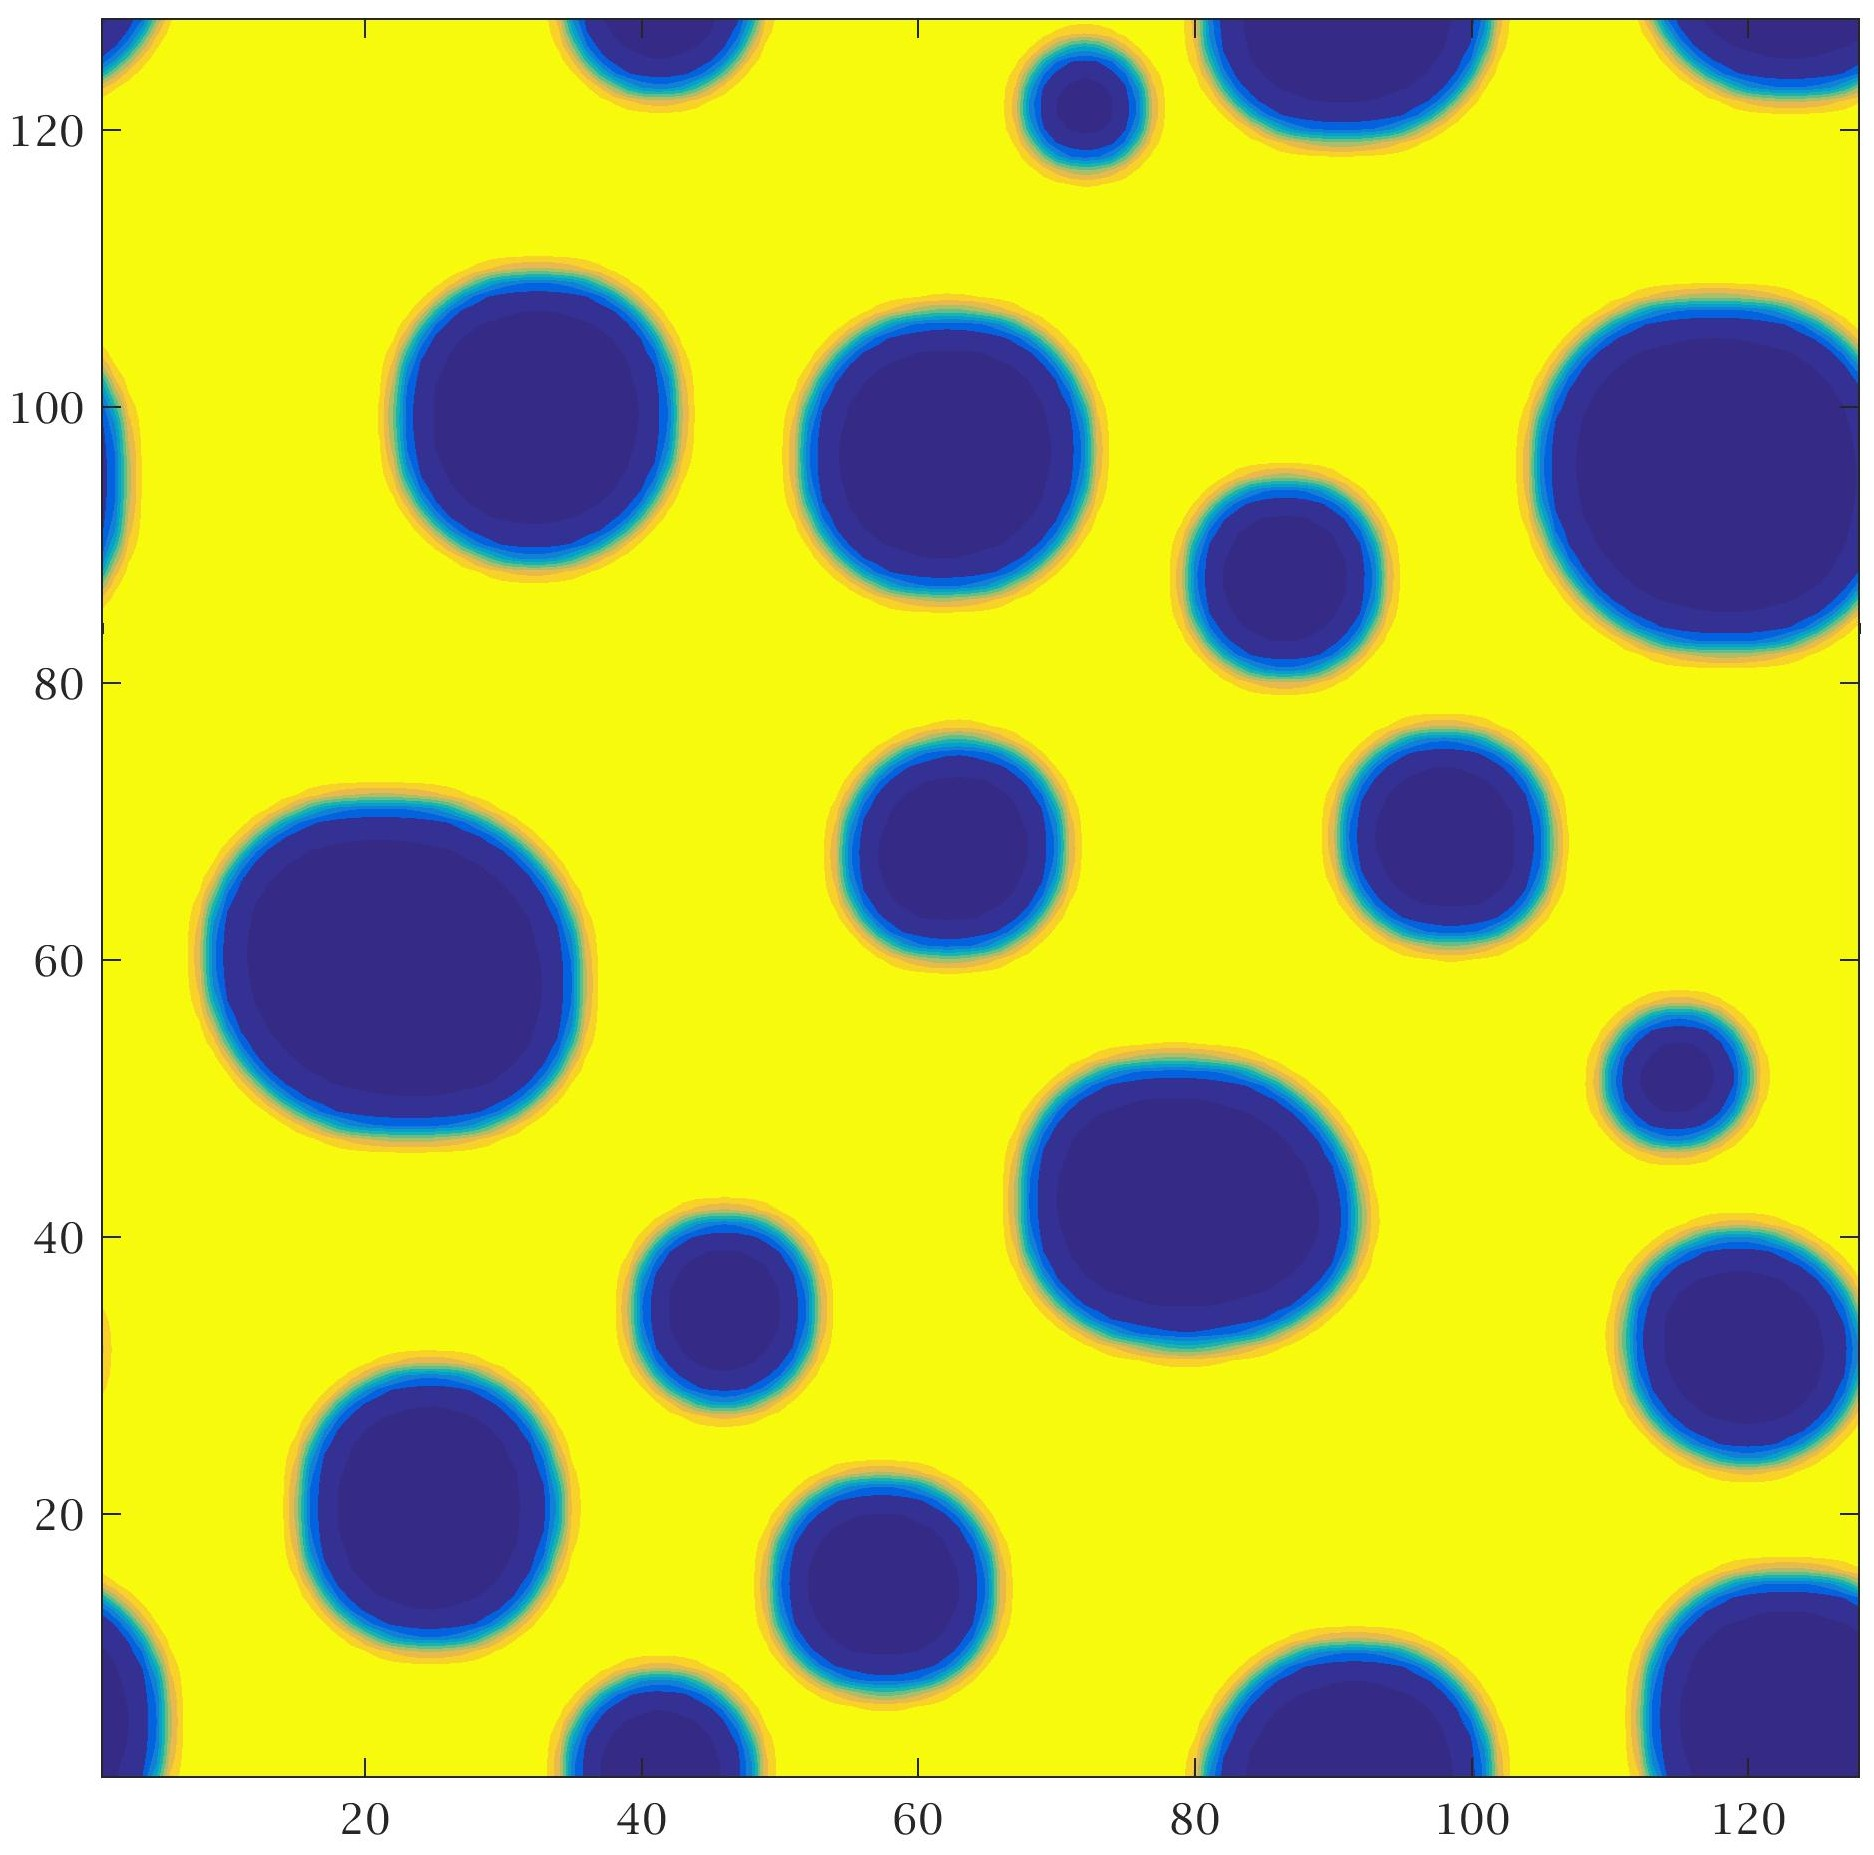
\includegraphics[width=1\textwidth]{pics/C3_t5.jpg}
                \subcaption{$t=200$}
        \end{minipage}
                \begin{minipage}[b]{.32\linewidth}
                \centering
                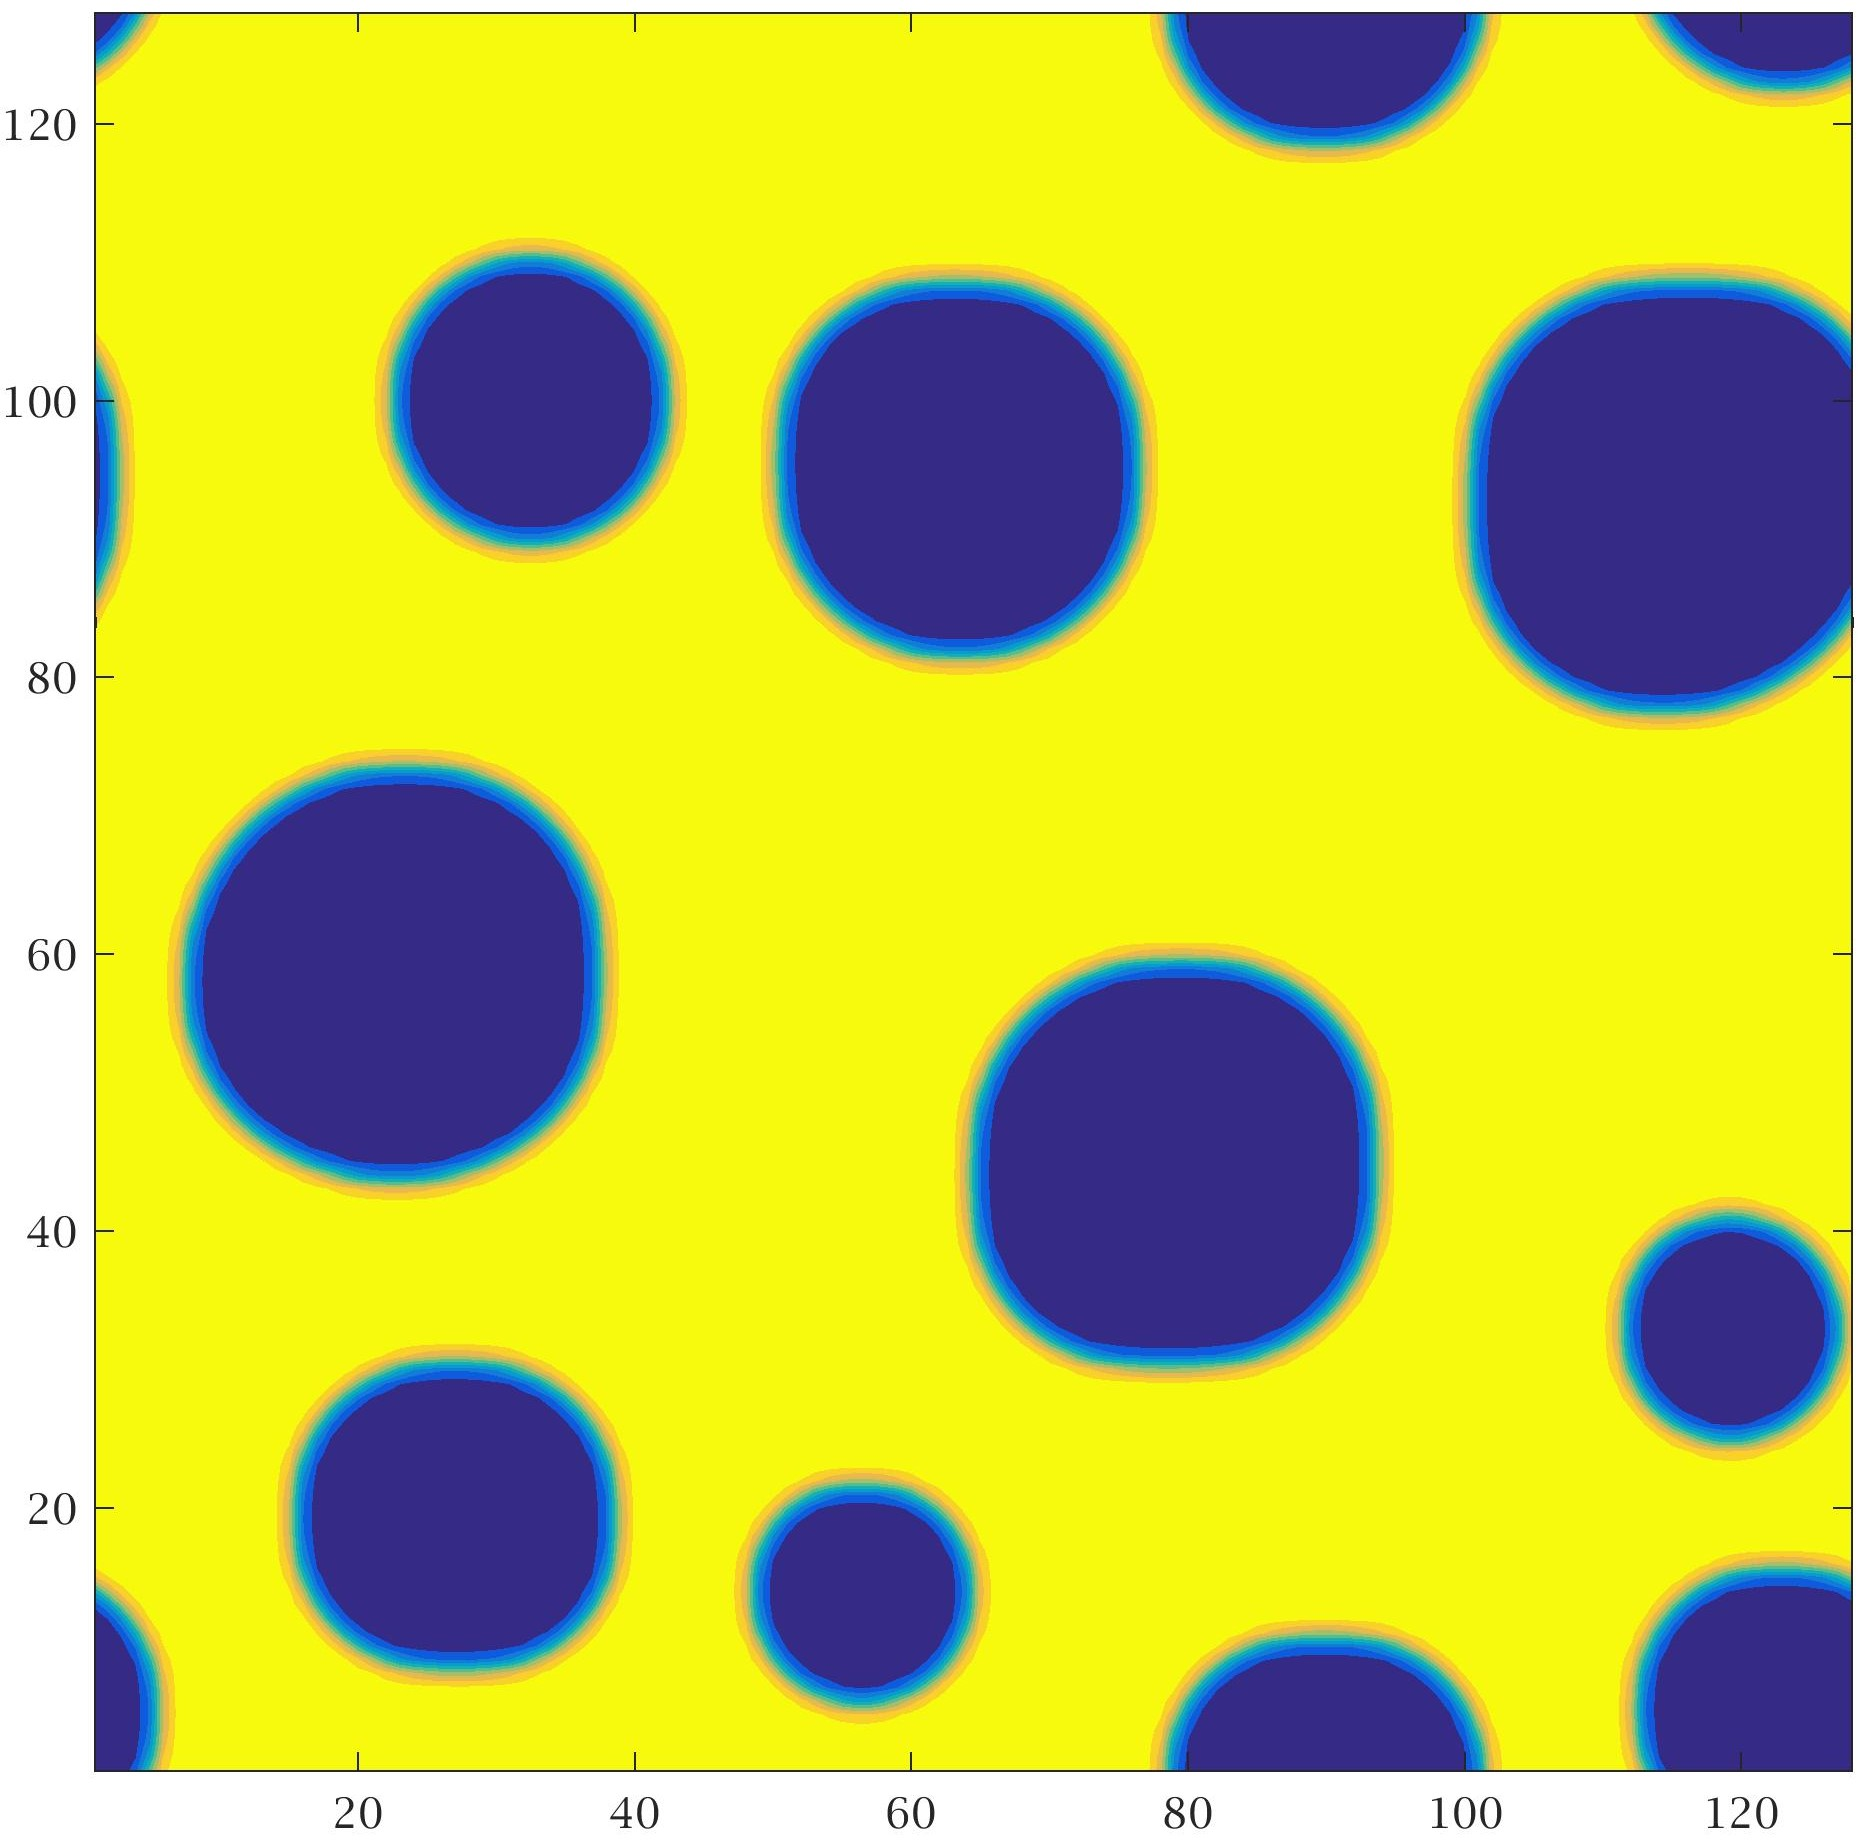
\includegraphics[width=1\textwidth]{pics/C3_t6.jpg}
                \subcaption{$t=500$}
        \end{minipage}
        \caption{Evolution with the average concentration of 0.7}
        \label{evolution_c3}
\end{figure}

Figures (\ref{E_c3} \& \ref{L_c3}) also shows the energy and characteristic length as the function of time for three different runs with the average concentration on 0.7.

Figure(\ref{E_c3}) also shows the energy decreases at a rate between $t^{-1/4}$ and $t^{-1/3}$; however, figure(\ref{L_c3}) shows that the characteristic length grows at a rate between $t^{1/4}$ and $t^{1/3}$.

\begin{figure}[H]
        \begin{minipage}[b]{.5\linewidth}        
                \centering
                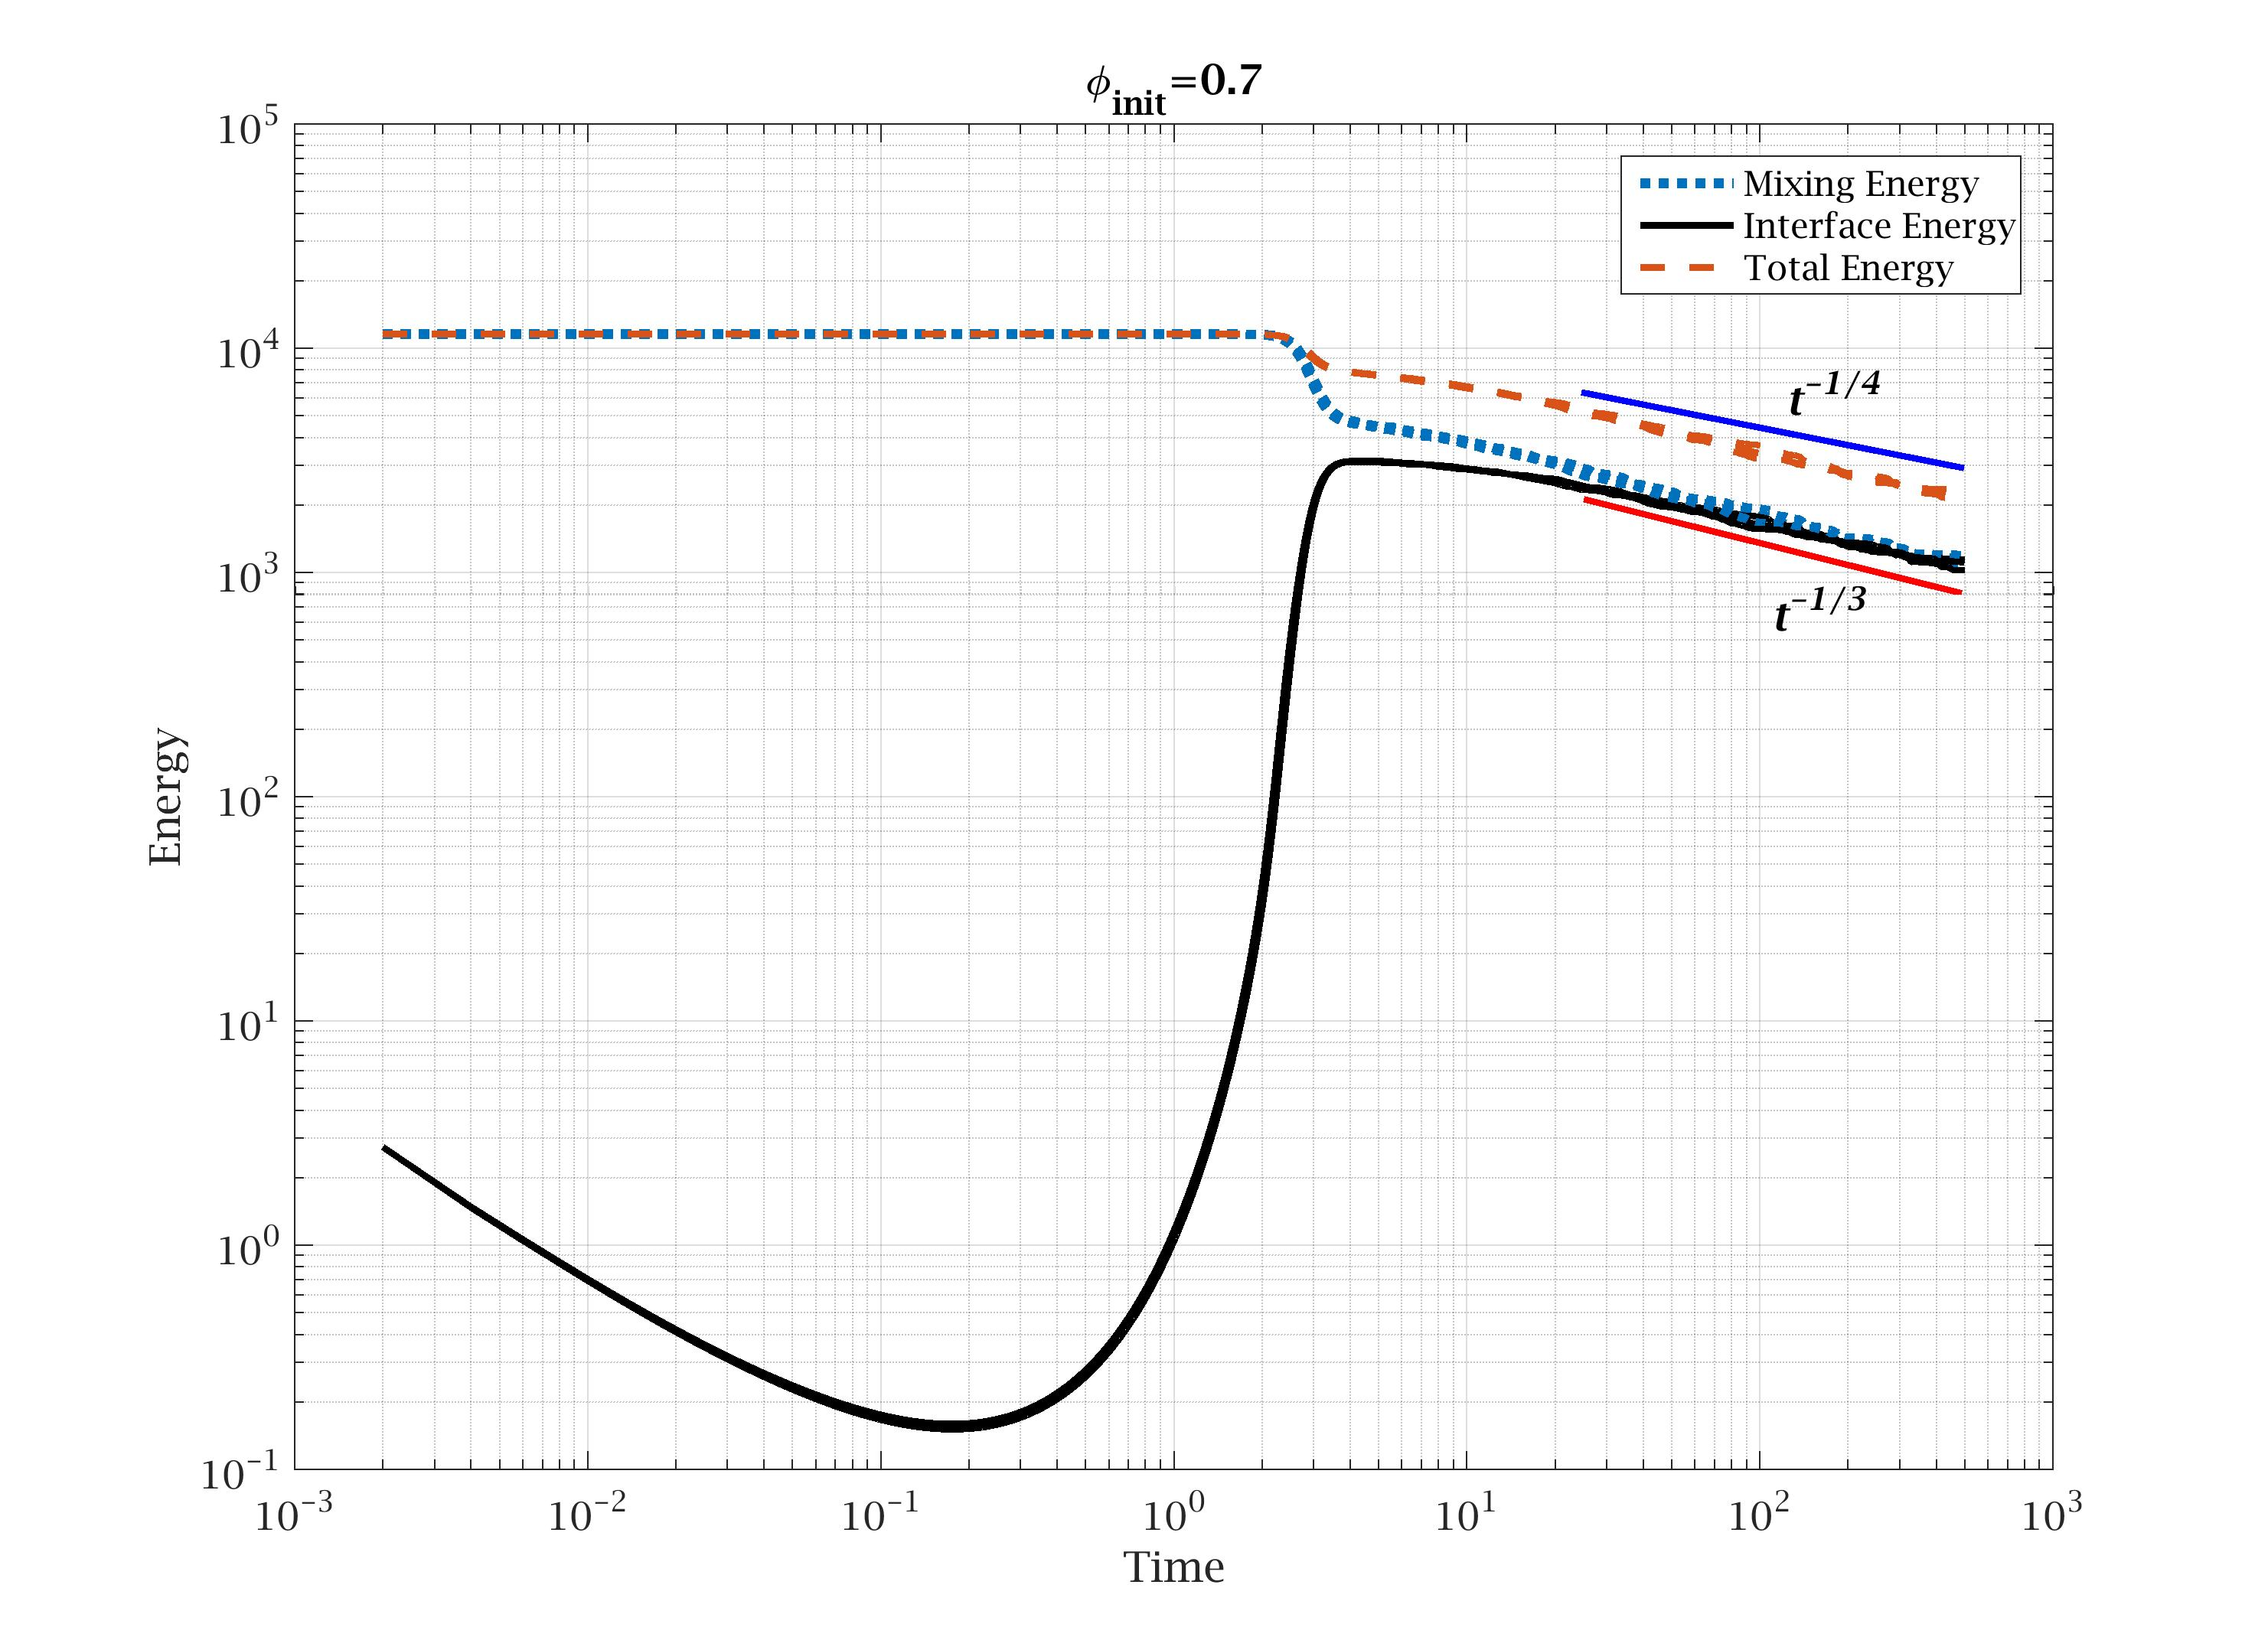
\includegraphics[width=1\textwidth]{pics/E_c3.jpg}
                \subcaption{}
                	\label{E_c3}
        \end{minipage}
        %   \hfill
        \begin{minipage}[b]{.5\linewidth}
                \centering
                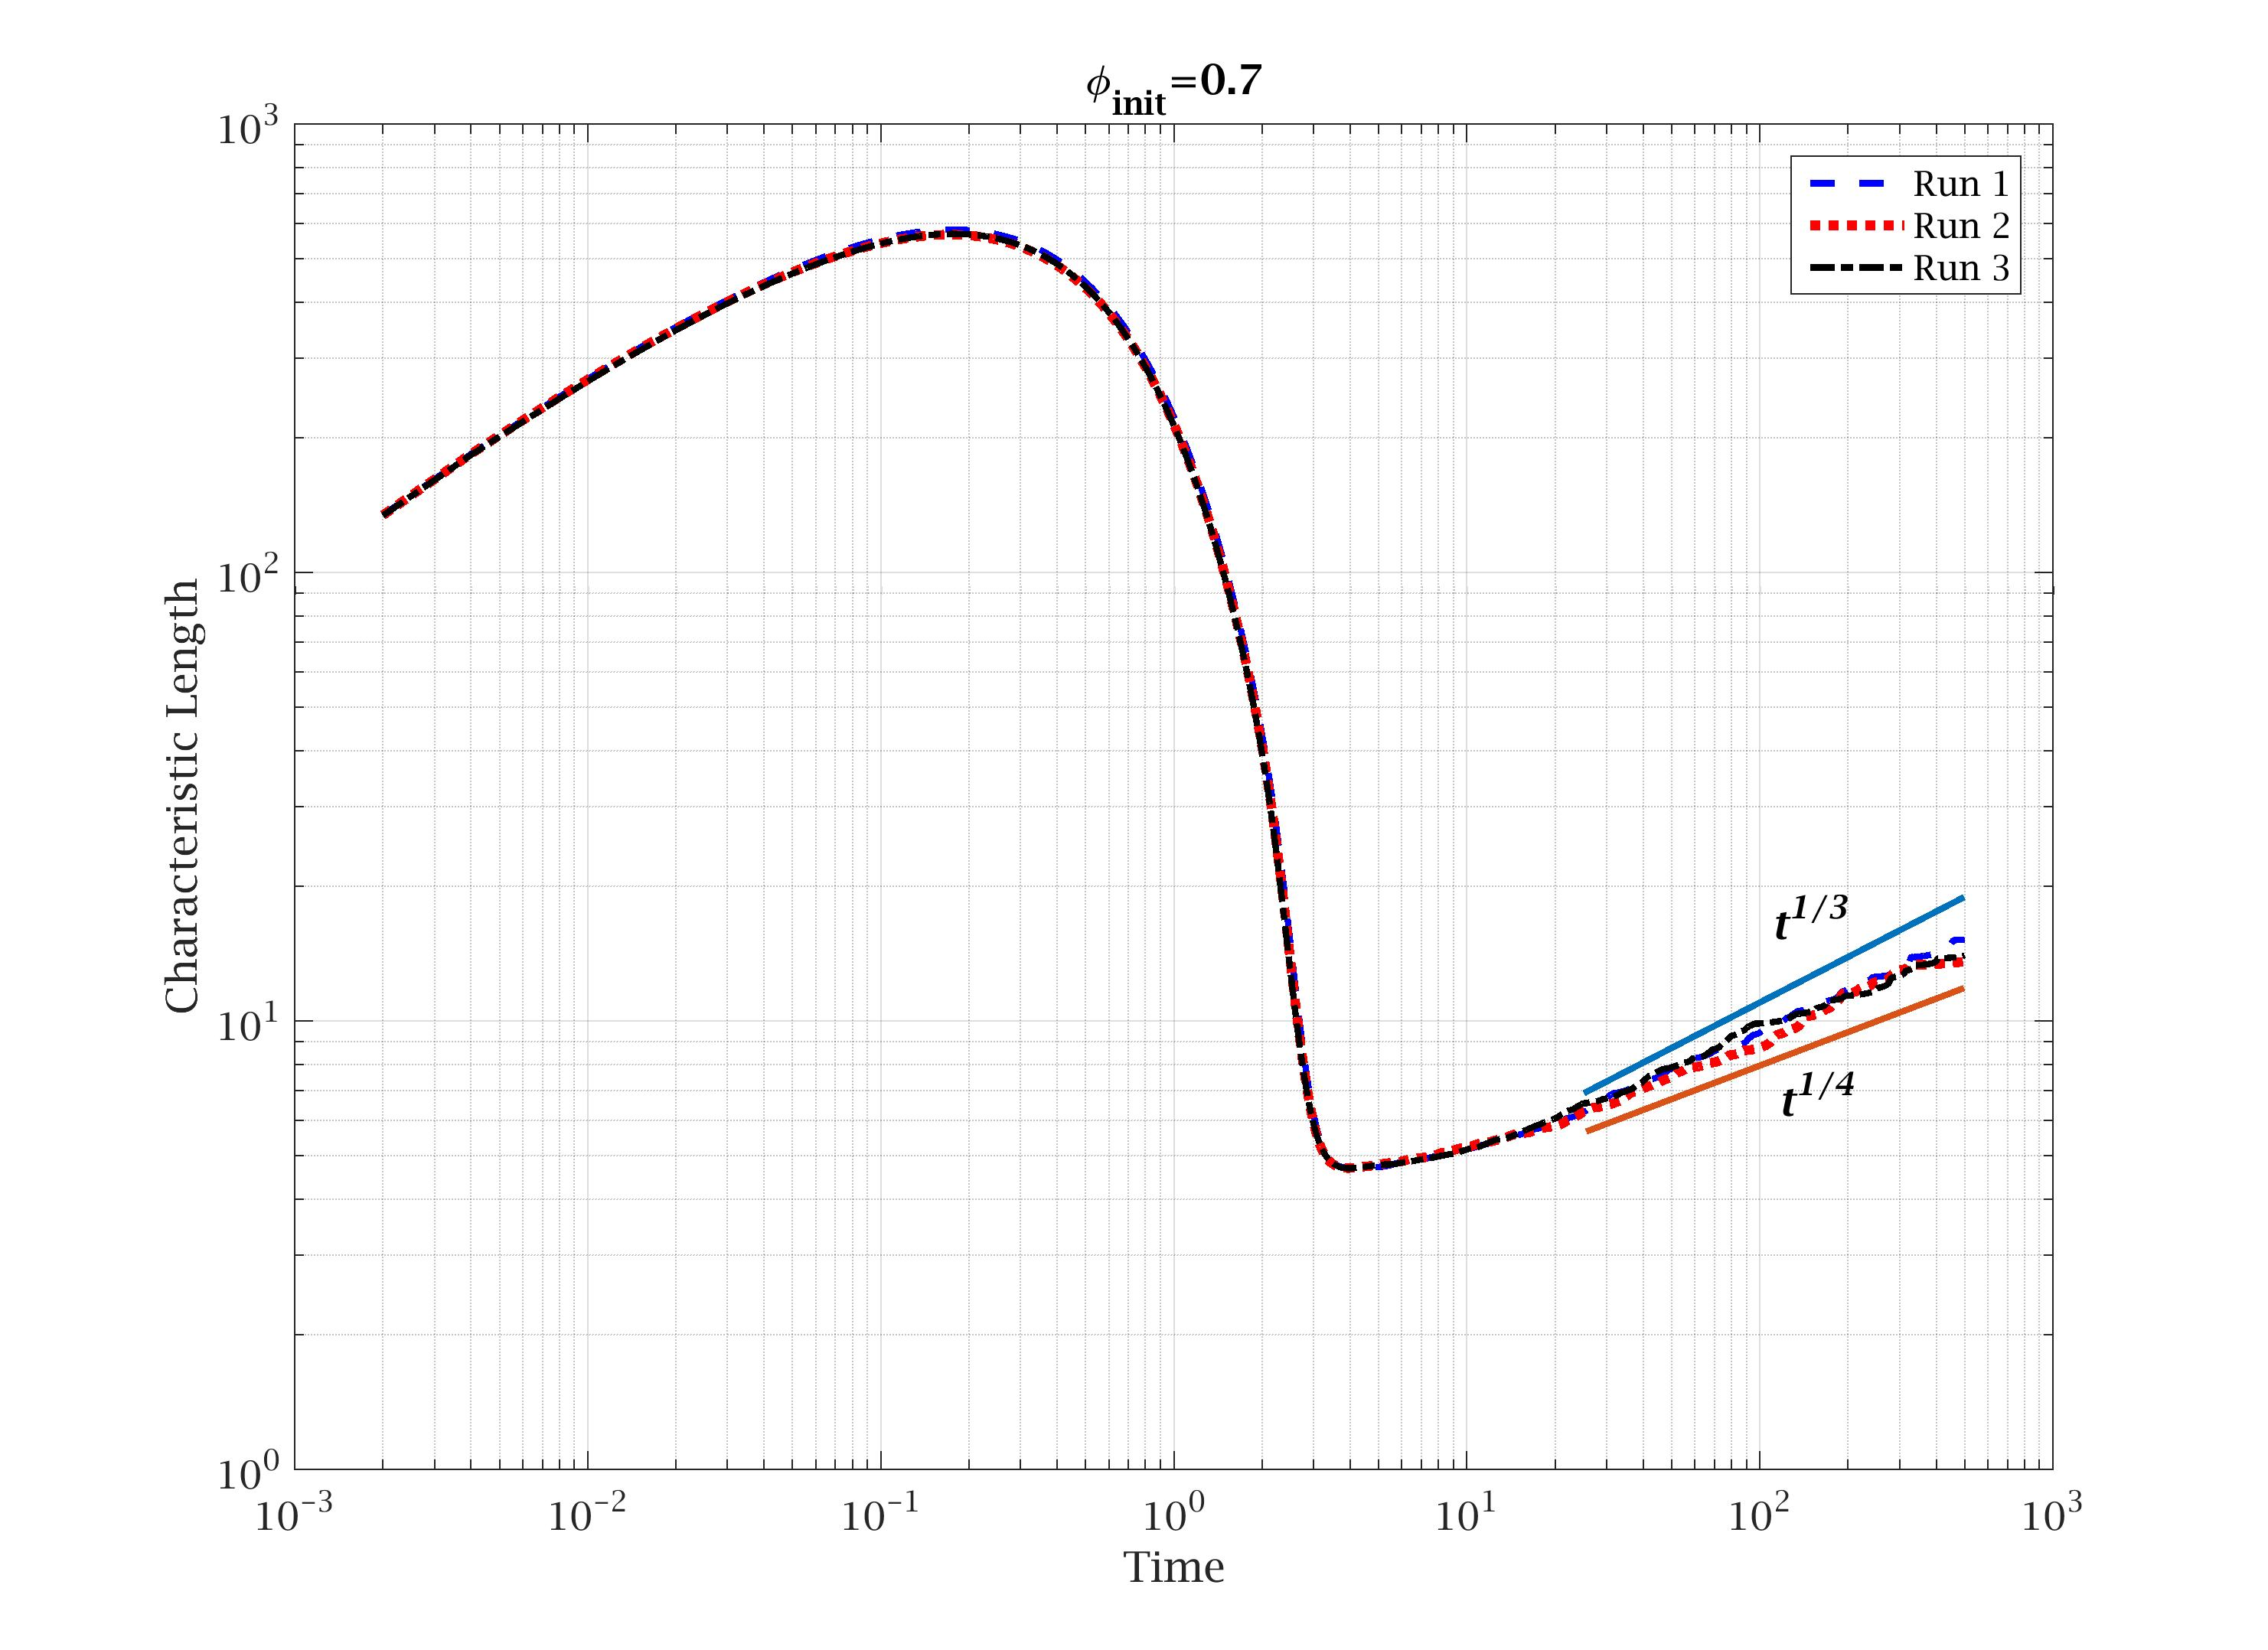
\includegraphics[width=1\textwidth]{pics/L_c3.jpg}
                \subcaption{}
                	\label{L_c3}
        \end{minipage}
                \caption{The (a) interfacial, mixing and total energy and (b) characteristic length as a function of time for the average concentration of 0.7}
        \label{EL_c3}
\end{figure}


\end{document}